%Document vide aux normes de l'École nationale des Chartes
%Dernières modifications E. Rouquette (12/2023)

%%%%%%%%%%%%%%%%%%%%%% PRÉAMBULE

%%%%%%%%%%%%%% partie obligatoire du préambule
\documentclass[a4paper,12pt,twoside]{book} % Définit la classe de document comme "book" avec des options : papier A4, taille de police 12pt, impression recto-verso

\usepackage{fontspec} % Permet l'utilisation de polices OpenType ou TrueType avec XeLaTeX ou LuaLaTeX
\usepackage{xunicode} % Facilite l'utilisation des caractères Unicode dans les documents, souvent utilisé avec fontspec (peut être redondant avec les versions modernes de fontspec)
\usepackage[french]{babel} % Configure les règles de typographie et la langue pour le français

%%%%%%%%%%%%%%%%%%%%%%%%%%%%%%%%% PACKAGES UTILISÉS
\usepackage{csquotes} % Permet l'utilisation des guillemets typographiques (français et autres) adaptés à la langue du document

\usepackage{lettrine} % Permet de créer des lettrines (initiales agrandies au début d'un paragraphe), ce n'est pas obligatoire mais peut être esthétique

\usepackage{graphicx} % Permet l'insertion et la gestion des images (pour redimensionner, faire pivoter, etc.)

\usepackage{subcaption} % Fournit des fonctionnalités pour ajouter des sous-légendes à des figures ou des tableaux contenant plusieurs sous-figures ou sous-tableaux

\usepackage{float} % Offre un meilleur contrôle sur le placement des figures et des tableaux avec des options comme [H] pour forcer le placement ici

\usepackage{fancybox} % Permet de dessiner des cadres décoratifs autour du texte ou des boîtes, comme des encadrements avec des ombres ou des formes spécifiques

\usepackage[table,xcdraw]{xcolor} % Fournit des outils pour colorier les tableaux et les lignes de code, avec l'option 'table' pour les tableaux et 'xcdraw' pour le dessin des couleurs dans les tableaux

\usepackage{listings} % Permet l'inclusion de code source avec mise en forme syntaxique, utile pour les documents techniques contenant du code

\usepackage{titling} % Permet une personnalisation avancée des titres du document, tels que le titre principal, le sous-titre, l'auteur, etc.

\usepackage{verbatim} % Permet d'inclure des blocs de texte brut (non interprété) tels qu'ils sont, souvent utilisé pour des commentaires ou des exemples de code

\usepackage{xcolor} % Permet l'utilisation des couleurs dans le texte, les tableaux, et autres éléments du document, comme la mise en forme du texte




\usepackage[style=enc,sorting=nyt,maxbibnames=10]{biblatex}%charger le style de l'EnC (téléchargeable ici https://ctan.org/pkg/biblatex-enc)
\addbibresource{biblio/bibli.bib} %le fichier bibliograhique. Exemple de chemin à partir du dossier où se trouve le document maître:Exemple ./dossierA/fichier.bib
%\defbibheading{}{\subsection*{}} Si l'on veut changer le titre de la/les bibliographie(s)


%%%Faire un ou plusieurs index

\usepackage{makeidx} %pour faire un ou plusieurs index
\makeindex  %commande pour générer l'index

%RAJOUTEZ ICI VOS PACKAGES
\lstset{
	backgroundcolor=\color{white}, % Couleur de fond
	frame=single,                  % Ajoute une bordure simple autour du code
	rulecolor=\color{black},       % Couleur de la bordure
	breaklines=true,               % Retourne à la ligne automatiquement
	basicstyle=\fontsize{5pt}{6pt}\selectfont\ttfamily, % Taille de police très réduite
	keywordstyle=\color{blue},     % Couleur des mots-clés
	commentstyle=\color{green},    % Couleur des commentaires
	stringstyle=\color{red},       % Couleur des chaînes de caractères
	numbers=left,                  % Position des numéros de ligne
	numberstyle=\tiny\color{gray}, % Style des numéros de ligne
	stepnumber=1,                  % Numérotation des lignes
	numbersep=5pt,                 % Distance entre les numéros et le texte
	showstringspaces=false         % Ne pas montrer les espaces dans les chaînes de caractères
}


%%%%%%%%%%%%%%%%%%%%%%%%%%%%%%%%% CONFIGURATION DE MISE EN PAGE

%%%%%% Les compteurs (sections, subsections, etc)
\renewcommand{\thesection}{\Roman{section}.}%On ne fait apparaître que le numéro de la section
\renewcommand{\thesubsection}{\arabic{subsection}.}%subsection en chiffres arabes
\renewcommand{\thesubsubsection}{\alph{subsubsection}.}%subsubsection en lettres minuscules
%Si l'on veut faire apparaître les subsubsection dans le table des matières (à commenter sinon)
\setcounter{tocdepth}{3}
\setcounter{secnumdepth}{3}  % La subsubsection (profondeur=3 dans la table des matières) apparait numérotée dans la TdM



%%%%%  Configurer le document selon les normes de l'école
\usepackage[margin=2.5cm]{geometry} %marges
\usepackage{setspace} % espacement qui permet ensuite de définir un interligne
\onehalfspacing % interligne de 1.5
\setlength\parindent{1cm} % indentation des paragraphes à 1 cm

%%%%% Mise en forme des headers (haut de page)
\usepackage{fancyhdr} %package utilisé pour modifier les headers
\pagestyle{fancy} %utiliser ses propres choix de mise en page et non ceux par défaut du package

\setlength\headheight{16pt}%la hauteur des headers
\renewcommand{\sectionmark}[1]{\markright{\small\textit{\thesection~\  #1}}}%Faire apparaître dans les headers les sections en  petit et en italiques
\renewcommand{\sectionmark}[1]{}%Commenter la lign précédetne et mettre celle-ci pour ne pas avoir le titre des sections dans le header
\renewcommand{\chaptermark}[1]{\markboth{\small\chaptername~\thechapter~--\ \textit{#1}}{}}%idem pour les chapitres
%\renewcommand{\chaptermark}[1]{}%Commenter la ligne précédente et mettre celle-ci pour ne pas avoir le titre des chapitres  dans le header



%indiquer des règles d'hyphénation pour des mots précis si besoin
%\begin{hyphenrules}{french}
%	\hyphenation{}
%\end{hyphenrules}


%%%%%%% Package hyperref
% A mettre après les autres appels de packages car redéfinit certaines commandes).

\usepackage[colorlinks=false, breaklinks=true, pdfusetitle, pdfsubject ={Mémoire TNAH}, pdfkeywords={les mots-clés}]{hyperref} %
\usepackage[numbered]{bookmark}%va avec hyperref; marche mieux pour les signets. l'option numbered: les signets dans le pdf sont numérotés

% Compléter pdfsubjet et pdfkeywords
%Explication des options de hyperref (modifiables)
% hyperindex=false
% colorlinks=false: pour que le cadre des liens n'apparaisse pas à l'impression
% breaklinks permet d'avoir des liens allant sur pusieurs lignes
%pdfusetitle: utiliser \author et \title pour produire le nom et le titre du pdf


%avec overleaf, utiliser :
%\usepackage[xetex]{hyperref}
%\hypersetup{
	%	pdfauthor = {Prénom Nom},
	%	pdftitle = {titre},
	%	pdfsubject = {sujet},
	%	pdfkeywords = {premier mot-clé} {deuxième mot-clé} {troisième mot-clé} {etc}
	%}



%%%%%%%%%%%%%%%%%%%% Package glossaries

%Exception: il faut le charger APRÈS hyperref
%\usepackage[toc=true]{glossaries}
%\makeglossaries
%avec TexStudio: F9 pour compiler le glossaire (s'il y a aussi un index)

%mettre les entrées du glossaire ici ou les mettre dans un fichier à part que l'on appelle ici par \loadglsentries{nom_du_fichier.tex}

%Structure d'une entrée de glossaire
%\newglossaryentry{}{%
%	name={},%
%	description={}
%}



%%%%%%%%%%%%%%%%%% DÉFINITION DES COMMANDES ET ENVIRONNMENTS






 %%%%%%%%%%%%%% INFORMATIONS POUR LA PAGE DE TITRE
\author{Léo Trotin - M2 TNAH}
\title{Mise en relation de deux bases de données en XML-TEI}

%%%%%%%%%%%%%%%%%%%%%% DOCUMENT
\begin{document}
	\begin{titlepage}
		\begin{center}
			
			\bigskip
			
			\begin{large}				
				ÉCOLE NATIONALE DES CHARTES\\
				UNIVERSITÉ PARIS, SCIENCES \& LETTRES
			\end{large}
			\begin{center}\rule{2cm}{0.02cm}\end{center}
			
			\bigskip
			\bigskip
			\bigskip
			\begin{Large}
				\textbf{Léo Trotin}\\
			\end{Large}
		%selon le cas
			\begin{normalsize} \textit{licencié ès lettres}\\
				\textit{diplômé de master}
			\end{normalsize}
			
			\bigskip
			\bigskip
			\bigskip
			
			\begin{Huge}
				\textbf{Mise en relation de deux bases de données de recherche en XML-TEI}\\
			\end{Huge}
			\bigskip
			\bigskip
			\begin{LARGE}
				\textbf{L'exemple de ThEMA et de SourcEncyMe}\\
			\end{LARGE}
			
			\bigskip
			\bigskip
			\bigskip
			\begin{large}
			\end{large}
			\vfill
			
			\begin{large}
				Mémoire 
				pour le diplôme de master \\
				\enquote{Technologies numériques appliquées à l'histoire} \\
				\bigskip
				2024
			\end{large}
			
		\end{center}
	\end{titlepage}

	\thispagestyle{empty}	
	\cleardoublepage
	
\frontmatter

	\chapter{Résumé}
\medskip
	Ce mémoire explore le processus de connexion entre deux bases de données de recherche en XML-TEI, SourcEncyMe et ThEMA, dans le but d'améliorer leur accessibilité et leur utilité pour la recherche scientifique. Le projet a débuté par une analyse des différentes méthodes de mise en relation, suivie d'une étude approfondie des deux bases pour garantir la qualité des données, déterminer les emplacements appropriés pour les liens dans les fichiers XML, et identifier les informations pertinentes à relier. Ensuite, diverses approches ont été examinées pour identifier les textes à connecter. Finalement, des liens ont été créés de manière semi-automatique entre les deux bases, et une indexation automatique des récits identifiés dans SourcEncyMe a été faite avec ThEMA. Cette interconnexion améliore non seulement l'accès à l'information, mais aussi la collaboration scientifique, valorise les données et ouvre de nouvelles perspectives pour la recherche.\\
	
	\textbf{Mots-clés:} Interopérabilité ; \index{XML-TEI}XML-TEI ; \index{Récits exemplaires}Récits exemplaires ; \index{Encyclopédies}Encyclopédies ; \index{XQuery}XQuery ; \index{Python}Python ; Automatisation ; ThEMA ; SourcEncyMe ; \index{Open Data}Open Data ;
	
	\
	
	\textbf{Informations bibliographiques:} Léo Trotin, \textit{Mise en relation de deux bases de données de recherche en \index{XML-TEI}XML-TEI. L'exemple de ThEMA et de SourcEncyMe}, mémoire de master \enquote{Technologies numériques appliquées à l'histoire}, dir. Enimie Rouquette, École nationale des chartes, 2024.
	
		\newpage{\pagestyle{empty}\cleardoublepage}
	
	\chapter{Remerciements}
	
\lettrine{J}e tiens à exprimer ma reconnaissance à ma directrice de mémoire, Enimie Rouqette, pour son encadrement et ses conseils tout au long de ce travail. Je remercie également Jean-Damien Genero, Jean-Paul Rehr et Emmanuelle Kuhry pour leur soutien en tant que tuteurs techniques. Je suis reconnaissant envers Marie-Anne Polo de Beaulieu et Isabelle Draelants pour leur direction scientifique. Mes remerciements vont aussi à l’équipe de l’EHESS et de l’IRHT pour leur accompagnement durant ce stage. Enfin, je remercie le LabEx HaStec pour le financement de ce projet.

\newpage{\pagestyle{empty}\cleardoublepage}


	
%%%%%%%%%%%% \bibliographie ici (normes de l'EnC)
\printbibliography[keyword={bibl},title={Bibliographie}]
\printbibliography[keyword={Web},title={Webographie}]
	
\chapter{Introduction}	
En 2011, lors d'un colloque sur les interactions entre le numérique et l'histoire, les chercheurs ont constaté que «~la discipline historique vit actuellement au moyen âge de son rapport à l'ordinateur, à la fois définitivement coupée des temps anciens (quand on travaillait «~sans~»), mais également marquée par le gothique des initiatives, désordonnées et tâtonnantes~». \footcite{thierryJeanPhilippeGenetAndrea2014a}. 

Depuis, la situation a évolué vers une uniformisation et un regroupement des productions numériques appliquées aux sciences sociales. Cela se manifeste, par exemple, par la création du portail Biblissima, qui propose un accès unifié à un ensemble de données numériques sur les manuscrits, incunables et imprimés anciens, provenant des neuf équipes partenaires du consortium Biblissima\footcite{PortailBiblissima}. De plus, l'importance croissante de l'interopérabilité et du  «~Linked \index{Open Data}Open Data~» dans le champ des humanités numériques, telle que constatée par Terhi Nurmikko-Fuller\footcite{nurmikko-fullerLinkedDataDigital2023}, témoigne également de cette évolution.

Cependant, il reste encore du travail à accomplir concernant les anciennes bases de données, qui n'ont pas été conçues à l'origine pour être interconnectées avec d'autres. C'est dans cette perspective que s'inscrit mon stage. Grâce au financement du \index{LabEx HaStec}LabEx HaStec, mon objectif a été de mettre en relation deux bases de données : ThEMA\footcite{ThEMA} et SourcEncyMe\footcite{SourcEncyMe}.


\section{Présentation des bases de données ThEMA et SourcEncyMe}
ThEMA peut se définir comme une base de données multimédia et multilingue sur des anecdotes exemplaires provenant principalement de l'Occident médiéval. Elle tire son origine d'un groupe de travail qui progressivement a enregistré des données au format Microsoft Word sur les \index{Récits exemplaires}récits exemplaires qui les intéressaient\footcite{rehrThesaurusExemplorumMedii2021a}. Ces fichiers sont repris dans les années 2000 par Marjorie Burghart pour créer une base de données PHP\footnote{Il s'agit d'un langage de script côté serveur utilisé pour le développement web. PHP peut être intégré dans le code HTML et est souvent utilisé pour créer des pages web dynamiques. Il permet de se connecter à une base de données MySQL pour manipuler les données (ajouter, modifier, supprimer, lire).} MySQL\footnote{Il s'agit d'un système de gestion de bases de données relationnelles (SGBDR) très populaire. Il permet de stocker, organiser et récupérer des données de manière efficace. MySQL utilise le langage SQL (Structured Query Language) pour gérer les bases de données.} avec une interface de saisie sous Microsoft Access qui permettait, hors ligne, le travail des indexateurs\footcite{burghartInformatisationThEMA2005}. Cette interface est ensuite remplacée par un site Web en 2005. Il est directement lié à une base de données MySQL. Ce type de bases permet une collaboration dynamique dans le contrôle de la qualité et la collecte des données. Le lancement de ce site a été rendu possible grâce aux efforts de Marjorie Burghart et de Pascal Collomb (EHESS), qui s'est intégré plus tardivement à l'équipe\footcite{rehrThesaurusExemplorumMedii2021a}. En 2015, Marjorie Burghart a suggéré de transférer le projet ThEMA à Huma-Num, une très grande infrastructure de recherche (TGIR) pour les sciences humaines financée par le CNRS, dans le but de garantir la sécurité à long terme de l'environnement du serveur\footcite{rehrThesaurusExemplorumMedii2021a}. Par la suite, la décision a été prise de développer un schéma \index{XML-TEI}XML-TEI pour les données de ThEMA et de les intégrer à un serveur d'application eXist-db, supervisés par Jean-Paul Rehr (université Lumière Lyon 2 et CIHAM), un outil qui a été lancé à l'automne 2019\footcite{rehrThesaurusExemplorumMedii2021a}.

ThEMA s'inscrit dans une longue tradition de bases de données créées par l'EHESS et le \index{CRH}CRH. Depuis les années 1960, le \index{CRH}CRH consacre une part importante de son activité à la constitution d'outils de recherche, mis à disposition de l'ensemble de la communauté savante\footcite{BasesDonneesTextuelles}. ThEMA est même la première base de données élaborée au sein de l’EHESS à avoir été mise en accès direct et libre\footcite{InformationsThEMA}. Actuellement, cette base est gérée d'un point de vue technique par Jean-Paul Rehr et Jean-Damien Généro, et d'un point de vue scientifique par \index{Marie-Anne Polo de Beaulieu}Marie-Anne Polo de Beaulieu. Elle est intégrée au collectif « Sources et données de la recherche », créé en 2019 pour accompagner les projets numériques du \index{CRH}CRH\footcite{SourcesDonneesRecherche}.

\

De son côté, SourcEncyMe se définit comme un corpus des \index{Encyclopédies}encyclopédies médiévales latines, où sont progressivement identifiées les sources grecques, arabes et latines de la pensée scientifique et philosophique. Cette base trouve ses origines dans l'« Atelier Vincent de Beauvais », qui, dès les années 1980, sous l'initiative du Doyen Jean Schneider et avec les efforts de Monique Paulmier-Foucart, assistée de Marie-Christine Duchenne, a entrepris la mise en ligne du \textit{Speculum historiale} de \index{Vincent de Beauvais}Vincent de Beauvais, sur le serveur du laboratoire ATILF à Nancy\footcite{SourcEncyMeSourcesEncyclopedies}. Le projet a pris de l'ampleur à partir de 2007 avec le développement d'un corpus de toutes les \index{Encyclopédies}encyclopédies latines médiévales, se transformant en 2010 en une base de données et une plateforme collaborative permettant l'enrichissement des données scientifiques\footcite{kuhryQuelsTraitementsNumeriques2022}. Le site SourcEncyMe.irht.cnrs.fr a été ouvert au public le 24 février 2016 à l’Institut de recherche et d’histoire des textes (IRHT, CNRS)\footcite{draelantsEncyclopediesMedievalesMilieu2022}. À partir de 2020, SourcEncyMe a subi une transformation technique, passant à un corpus intégré en \index{XML-TEI}XML-TEI avec une base de données unifiée en XML, associée à la création d’une interface de balisage\footcite{draelantsEncyclopediesMedievalesMilieu2022}.

Aujourd'hui, SourcEncyMe est l'une des nombreuses bases de données gérées par l'\index{IRHT}IRHT, un institut qui a été parmi les premiers à adopter les progrès techniques du numérique pour le traitement des sources historiques\footcite{holtzIRHTAuFil2015}. La base fait partie du pôle numérique de l'institut, lequel vise à assurer l’interopérabilité, la diffusion, la valorisation et l’enrichissement des données issues de la recherche\footcite{PoleNumerique}. D'un point de vue technique, SourcEncyMe est gérée par Henri Seng et \index{Emmanuelle Kuhry}Emmanuelle Kuhry, tandis que la gestion scientifique est assurée par \index{Isabelle Draelants}Isabelle Draelants.


\section{Motivations et enjeux de l'interconnexion des bases de données}
Bien que ThEMA et SourcEncyMe soient des entités distinctes avec des histoires, des institutions d'attache et des sources différentes, plusieurs points communs permettent d'envisager leur interconnexion.

D'un point de vue historique, les recueils d'\textit{exempla} et les encyclopédies participent tous deux à l’encyclopédisme du XIIIe siècle\footcite{legoffPourquoiXIIIeSiecle1994}. Par exemple, un même auteur, comme Thomas de Cantimpré, a pu rédiger à la fois une encyclopédie (\textit{De natura rerum}) et un recueil de récits exemplaires (\textit{Bonum universale de apibus}). Ces œuvres partagent une rhétorique commune visant à décoder l'œuvre de Dieu sur Terre. De plus, les \index{Encyclopédies}encyclopédies et les recueils d'\textit{exempla} se réfèrent respectivement à leur contenu. Par exemple, des éléments du \textit{Speculum majus} de \index{Vincent de Beauvais}Vincent de Beauvais ont été repris dans 28 recueils de \index{Récits exemplaires}récits exemplaires entre le XIIIe et le XVe siècle\footcite{berliozRecueilsExemplaDiffusion1994}.

D'un point de vue technique, les textes des deux bases sont encodés en \index{XML-TEI}XML-TEI, un format de balisage spécifique pour les documents textuels. Ce format permet à l'information d'avoir exactement le même aspect pour tous les logiciels qui l'utilisent, même si la structure du XML peut différer\footcite{burnardQuEstceQue2015}. De plus, les systèmes de gestion de bases de données (\index{SGBD}SGBD) utilisés, BaseX et eXist-db, sont très similaires. Ces \index{SGBD}SGBD stockent les données XML sous forme native, utilisent \index{XQuery}XQuery comme langage de requête principal, et sont dotés de licences offrant une grande liberté d'utilisation et de modification. Enfin, même l'interface visuelle des deux bases présente des ressemblances : \\

% Première figure
\begin{figure}[H]
	\centering
	\fbox{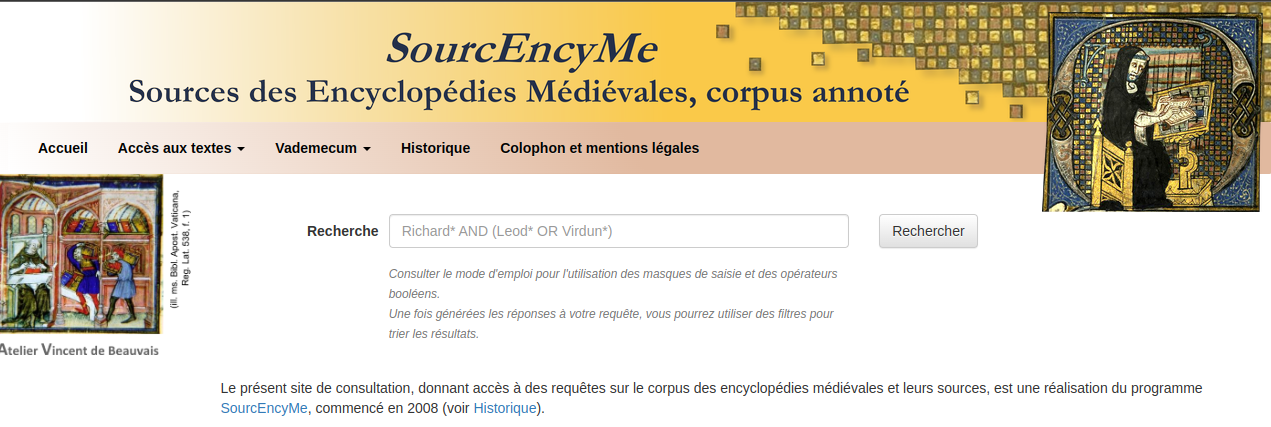
\includegraphics[width=0.8\linewidth]{images/visuel_sourcencyme.png}}
	\caption{Page d'accueil de SourcEncyMe}
\end{figure}

\vspace{10pt} % Espacement vertical entre les figures

% Deuxième figure
\begin{figure}[H]
	\centering
	\fbox{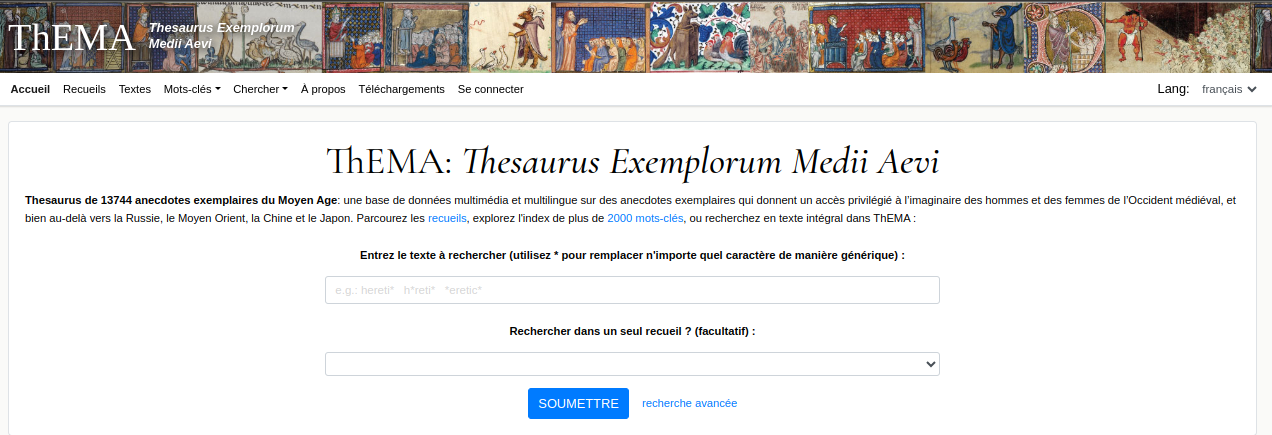
\includegraphics[width=0.8\linewidth]{images/visuel_thema.png}}
	\caption{Page d'accueil de ThEMA}
\end{figure}

D'un point de vue scientifique, les deux projets partagent une vocation commune : rendre accessible un patrimoine ancien et précieux pour comprendre le répertoire des connaissances médiévales et les informations sur la vie matérielle au Moyen Âge. Ils intègrent les textes dans une histoire de la transmission des savoirs, en accordant une attention particulière aux métadonnées qui indiquent la source des textes et les textes apparentés.

D'un point de vue institutionnel, l'\index{EHESS}EHESS et l'\index{IRHT}IRHT entretiennent de bonnes relations\footcite{holtzInstitutRechercheHistoire2005}. Des chercheurs des deux institutions participent à des projets communs, bien qu'ils soient parfois en concurrence. C'est le cas de \index{Marie-Anne Polo de Beaulieu}Marie-Anne Polo de Beaulieu pour ThEMA et d'\index{Isabelle Draelants}Isabelle Draelants pour SourcEncyMe, qui sont toutes deux impliquées dans le \index{LabEx HaStec}LabEx HaStec, un laboratoire d'excellence se concentrant sur les savoirs, les techniques et les croyances, des thèmes bien représentés dans les deux bases de données\footcite{LabexHastecEPHE}. Ce type de projet est crucial car il favorise la création de liens entre les institutions. Grâce au financement du \index{LabEx HaStec}LabEx HaStec, j'ai ainsi pu réaliser ce stage, permettant ainsi aux équipes des deux projets de se rencontrer. Le \index{LabEx HaStec}LabEx HaStec a également financé une post-doctorante, Élisa Lonati, qui travaillera aussi à cheval entre ThEMA et SourcEncyMe, assurant la continuité des liens établis entre les deux équipes.

\section{Présentation de la problématique et du plan}

L'interopérabilité est devenue un enjeu majeur en sciences sociales ces dernières années, comme mentionné précédemment. Elle est essentielle pour rendre les données de recherche accessibles dans un environnement universitaire fragmenté, où les intérêts scientifiques varient, les sources historiques sont dispersées, et les bases de données souvent isolées. Toutefois, grâce à la convergence des efforts de certains chercheurs, cet objectif reste réalisable. La question que je vais explorer est donc la suivante : comment connecter efficacement deux systèmes de gestion de bases de données (\index{SGBD}SGBD) en \index{XML-TEI}XML-TEI, qui, bien que distincts, présentent des similarités ?

Pour répondre à cette problématique, j'examinerai d'abord les différentes options disponibles et la modalité choisie pour mettre en relation les deux bases de données. Ensuite, je détaillerai la mise en œuvre concrète de cette connexion.Enfin, je prendrai du recul sur ce travail de connexion pour évaluer ses apports et ses perspectives.


\newpage{\pagestyle{empty}\cleardoublepage}

%%%%%%%%%%%%%%%%%Le corps du mémoire
	\mainmatter
%Trier par dossiers si besoin (front, main,annexes,), se crérer un docuemnt .tex par structure (section ou chapter selon la taille et la pertinence) Exemple de chemin à partir du dossier où se trouve le document maître: ./dossierA/fichier.tex

\chapter{Réflexions sur les différentes possibilités d'interconnexion}
Pour établir une interconnexion efficace entre les bases de données ThEMA et SourcEncyMe, trois solutions ont été envisagées : la fusion des bases de données, la création d'une API, et l'ajout de liens simples dans les fichiers \index{XML-TEI}XML-TEI. Chacune de ces solutions présente des avantages et des inconvénients, tant sur le plan technique qu'institutionnel et scientifique.


\section{Solution radicale : fusionner les deux bases de données}
L'une des solutions les plus directes pour relier ThEMA et SourcEncyMe consiste à fusionner les deux bases de données en un projet unique. Cette option pourrait être envisagée en regroupant les deux bases sous l'égide d'une infrastructure commune, telle que Biblissima, puisque l'IRHT et l'EHESS sont déjà partenaires de ce projet\footcite{PartenairesProjetBiblissima}. Une autre possibilité serait de les fusionner directement dans ThEMA ou SourcEncyMe. 

La fusion des deux bases de données présente plusieurs avantages. Tout d'abord, elle élimine la nécessité de développer une API, ce qui pourrait simplifier considérablement le processus d'interconnexion. En outre, en consolidant les deux systèmes de gestion de bases de données (\index{SGBD}SGBD), la maintenance serait également simplifiée, car une seule base de données nécessiterait une gestion continue.

Cependant, cette solution présente des inconvénients. Sur le plan institutionnel, la fusion impliquerait que l'une des deux institutions, l'EHESS ou l'IRHT, prenne en charge l'ensemble du travail de gestion des deux bases, ce qui pourrait poser des problèmes de responsabilité et de gouvernance. D'un point de vue historique, la fusion risquerait de brouiller la distinction entre les deux types de sources que sont les \index{Encyclopédies}encyclopédies et les récits exemplaires. Enfin, sur le plan scientifique, bien que les deux bases poursuivent des objectifs similaires en termes de valorisation du patrimoine médiéval, ThEMA se concentre sur la diversité des \index{Récits exemplaires}récits exemplaires\footcite{ThEMA}, tandis que SourcEncyMe se focalise sur la transmission des textes encyclopédiques\footcite{SourcEncyMe}. Ces différences essentielles seraient potentiellement compromises par une fusion.

Face à ces défis, il a été nécessaire de considérer d'autres solutions moins radicales et plus respectueuses des spécificités institutionnelles et scientifiques de chaque base.


\section{Solution idéale : développer une API}
La création d'une \index{API}API (Interface de Programmation d'Applications) permettrait de connecter les deux bases tout en les maintenant distinctes. Une \index{API}API est un ensemble de spécifications techniques permettant à des logiciels de communiquer entre eux en définissant des protocoles, méthodes, et formats de données. Cette solution offrirait un point d'accès centralisé pour interroger les deux bases, et permettrait de manipuler des données provenant de schémas \index{XML}XML différents, même si ces schémas évoluent\footcite{pedroBuildingAPIProduct2024}.

L'avantage de cette approche est de pouvoir, par exemple, rechercher un \textit{exemplum} dans SourcEncyMe et récupérer les \index{Récits exemplaires}récits exemplaires similaires dans ThEMA en utilisant l'indexation de l'\textit{Index exemplorum} de Frederic Tubach\footcite{tubachIndexExemplorumHandbook1969}, sans avoir à recréer un système d'indexation des \textit{exempla} dans SourcEncyMe\footnote{L'ouvrage de Tubach, publié en 1969, propose une classification et un catalogue des récits exemplaires en fonction de leurs thèmes, motifs et caractéristiques. Il est intégré à ThEMA.}.

Cette solution maintient la distinction historique entre les sources et respecte les spécificités scientifiques et institutionnelles des deux bases. Cependant, elle a été écartée en raison de la complexité technique et du temps limité du stage. ThEMA dispose déjà d'une API, mais SourcEncyMe n'en avait pas, et je n'avais pas accès direct au code source, seulement aux fichiers contenant les \index{Encyclopédies}encyclopédies.

Ces contraintes nous ont conduits à opter pour une dernière option : l'ajout de simples liens dans les fichiers XML.


\section{Un compromis : l'ajout de liens simples}
La solution finalement retenue pour l'interconnexion des deux bases de données a consisté à ajouter de simples liens dans les fichiers \index{XML-TEI}XML-TEI. Cette approche, bien que techniquement moins ambitieuse que la création d'une \index{API}API ou la fusion des bases, présente plusieurs avantages.

L'ajout de liens est une tâche relativement simple à mettre en œuvre. Il s'agit d'insérer des balises \index{XML-TEI}XML-TEI qui pointent vers des données similaires présentes dans les deux bases. Ces liens peuvent ensuite être activés dans le HTML des bases de données, permettant aux utilisateurs de naviguer facilement entre ThEMA et SourcEncyMe.

Cette solution présente l'avantage d'être facilement réalisable dans le cadre d'un stage court et de ne nécessiter qu'une formation technique limitée. De plus, elle évite les conflits institutionnels, scientifiques et historiques, car les deux bases restent distinctes tout en étant reliées. Ainsi, cette méthode offre un bon compromis, permettant d'interconnecter les deux bases de manière efficace sans compromettre leur indépendance. %Input: importer un fichier

\chapter{Stratégies pour l'intégration des liens dans les deux bases de données}
Avant d'établir les liens entre les bases de données, il est essentiel de préparer correctement ces bases. Cela inclut la vérification de la qualité et de la pérennité des données, ainsi que la planification précise de l'insertion des liens dans les fichiers \index{XML}XML et des données ou métadonnées à associer.


\section{Vérification de la qualité des données et de leur pérennité}
Je me suis principalement chargé de la vérification de la qualité des données et de la pérennité de ThEMA, car je n'ai pas eu de tâches similaires du côté de SourcEncyMe.

\

J'ai d'abord rédigé une documentation détaillée sur le fonctionnement et l'installation locale de la base de données. Ce travail, présenté dans les annexes A et B, est crucial pour éviter l'abandon des bases de données lorsque les chercheurs responsables prennent leur retraite. La disparition éventuelle de la base compromettrait la valeur des liens créés. Ce point est d'autant plus pertinent avec le départ prochain à la retraite de \index{Marie-Anne Polo de Beaulieu}Marie-Anne Polo de Beaulieu, directrice scientifique du projet. Il est impératif que cette documentation facilite le transfert de connaissances aux futurs chercheurs ou ingénieurs d'études qui reprendront ThEMA. Actuellement, Jean-Paul Rehr, le créateur de la base, en assure seul la gestion. Il est donc essentiel que ses connaissances soient préservées.

J'ai également résolu un problème lié à l'affichage des \textit{exempla}. Initialement, les \textit{exempla} n'étaient pas classés selon l'ordre du recueil, mais étaient triés en fonction du numéro du fichier XML. Par exemple, un \textit{exemplum} numéroté 10 pourrait apparaître avant un \textit{exemplum} 5.2 si ce dernier avait été ajouté ultérieurement, car son fichier \index{XML}XML avait été généré plus tard. De plus, des incohérences liées aux différentes méthodes d'indexation utilisées par les chercheurs ont été identifiées : certains \textit{exempla} étaient classés avec des notations variées telles que 1.b; 1b; 1, 5, 6. Cette diversité de formats empêchait un classement croissant uniforme. La réorganisation était donc nécessaire pour garantir que les utilisateurs puissent retrouver facilement les \textit{exempla} recherchés. Sans cette réorganisation, les liens vers SourcEncyMe risquaient de devenir moins accessibles. \\

\begin{figure}[H]
	\centering
	\fbox{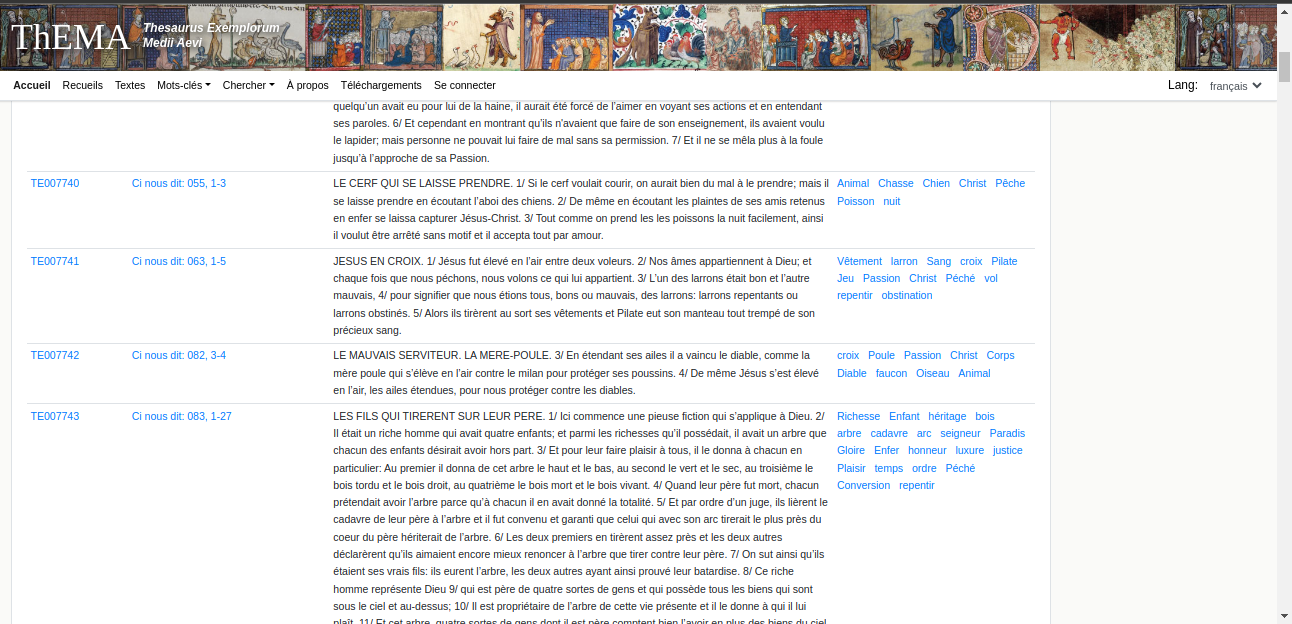
\includegraphics[width=0.8\linewidth]{images/recitsmalclasses.png}}
	\caption{Récits exemplaires mal classés}
\end{figure}

Pour résoudre ce problème, j'ai d'abord développé un code en \index{Python}Python (annexe C). Ce code extrait les numéros des \index{Récits exemplaires}récits exemplaires et convertit les lettres présentes dans la numérotation en chiffres. Cependant, cette méthode a présenté des inconvénients : elle nécessitait de modifier de nombreux types de numérotations et de réintégrer les fichiers \index{XML}XML modifiés dans la base, alors que seulement 30 \% des récits étaient mal classés.

Une approche plus simple a donc été développée pour identifier uniquement les recueils présentant des erreurs de classement et les corriger sans tenter d'uniformiser les numéros des récits. De plus, ce second code a été écrit en \index{XQuery}XQuery (annexe D) afin de s'intégrer directement dans la base de données. Ainsi, en cas de nouvelles erreurs d'indexation, elles seront automatiquement traitées, éliminant la nécessité de relancer le code \index{Python}Python et de réintégrer les données dans la base.


\section{Identifications des liens entre les bases de données}
J'ai identifié des similitudes entre les deux bases de données, tant au niveau des données que des métadonnées. Pour les données, c’est-à-dire les éléments bruts susceptibles de fournir des informations (ici, tu texte), les types de connexions possibles sont les suivants : \\

\begin{itemize}
	\item Quand un \textit{exemplum} d'un recueil de récits exemplaires utilise un morceau d'une \index{Encyclopédies}encyclopédie.
	\item Quand un \textit{exemplum} est repéré dans une encyclopédie et qu'un recueil d'\textit{exempla} contient un \textit{exemplum} similaire ou si on le retrouve dans la classification de l'\textit{Index exemplorum} de Frederic Tubach.
	\item Quand un \textit{exemplum} est identifié dans une encyclopédie et qu'il est indexé dans ThEMA.
\end{itemize}

\

Pour ce qui est des métadonnées, qui fournissent des informations sur d'autres données, voici les éléments pouvant être connectés : \\

\begin{itemize} 
	\item Les \index{Mementos}mementos (fiches de présentation des auteurs ou des œuvres) des deux bases de données et leur contenu respectif peuvent être connectés : \\
	
	\begin{figure}[H]
		\centering
		\fbox{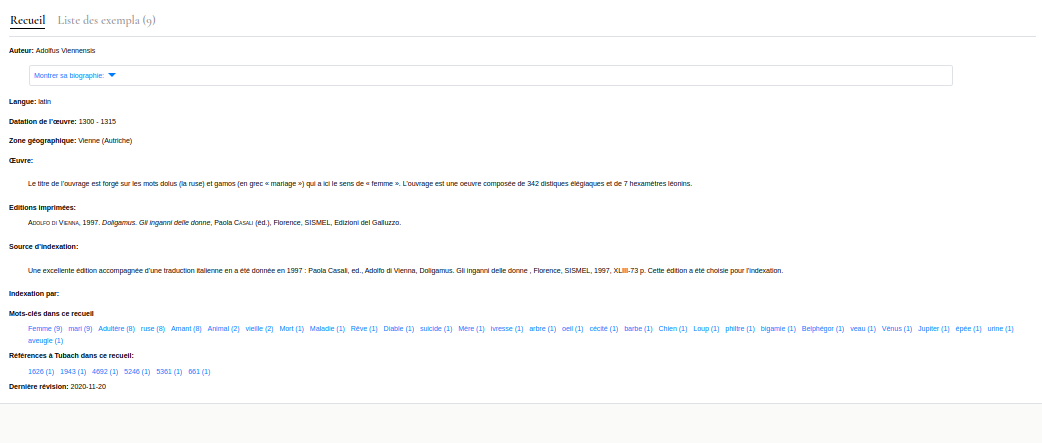
\includegraphics[width=0.8\linewidth]{images/mementothema.png}}
		\caption{Memento dans ThEMA}
	\end{figure}
	
	\begin{figure}[H]
		\centering
		\fbox{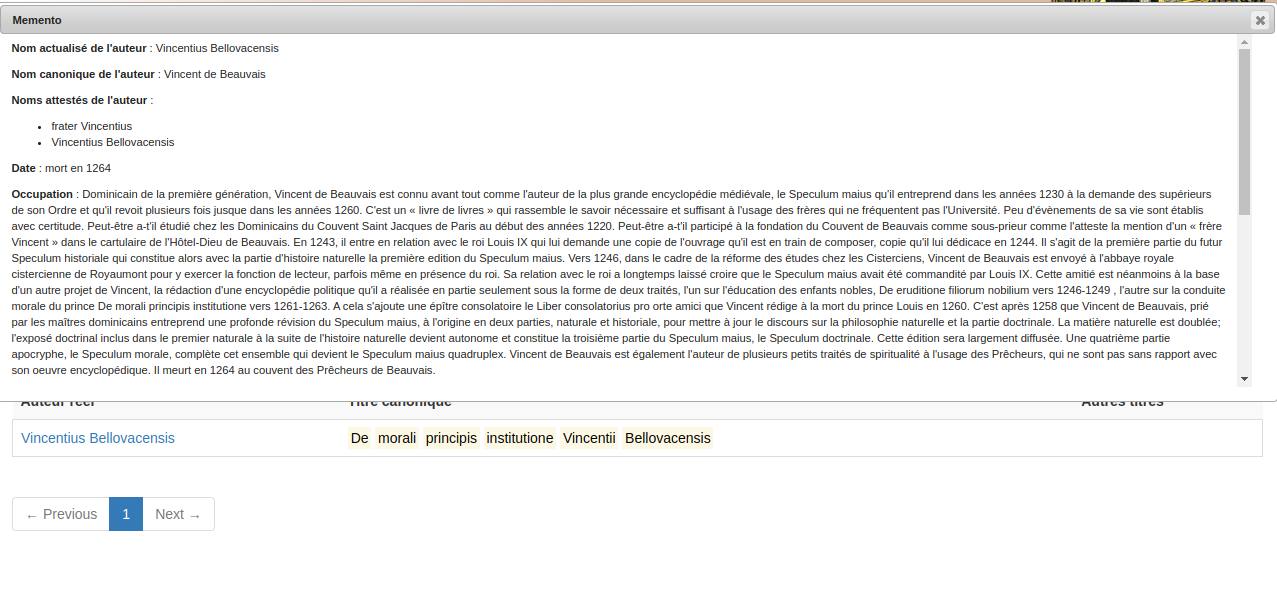
\includegraphics[width=0.8\linewidth]{images/mementosourcencyme.png}}
		\caption{Memento dans SourcEncyMe}
	\end{figure}
	
	\item Les sources des \index{Récits exemplaires}récits exemplaires mentionnées lors de l'indexation sur ThEMA peuvent être connectées aux \index{Mementos}mementos, comme illustré avec Cicéron : \\

	\begin{figure}[H]
		\centering
		\fbox{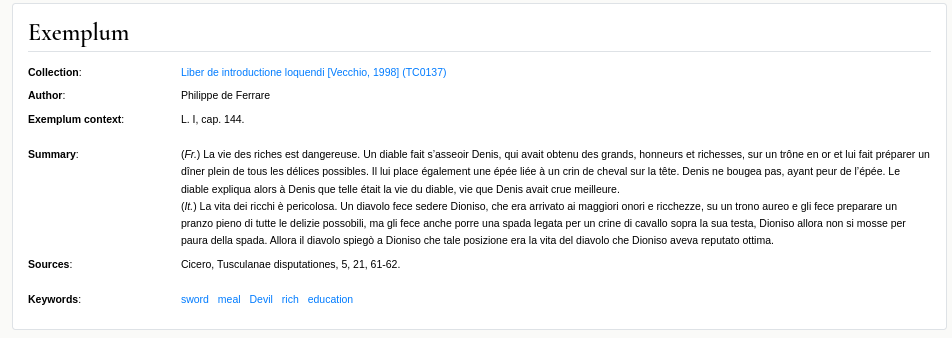
\includegraphics[width=0.8\linewidth]{images/sourcethemacicero.png}}
		\caption{Récit exemplaire utilisant un texte de Cicéron}
	\end{figure}

	\begin{figure}[H]
		\centering
		\fbox{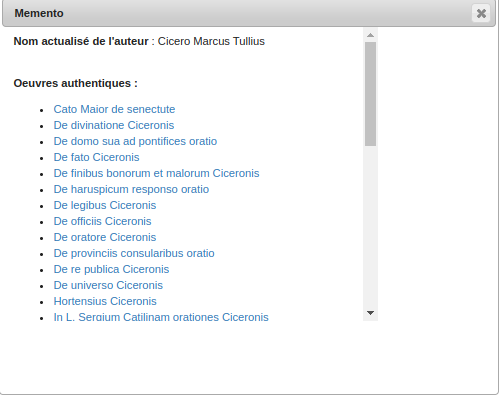
\includegraphics[width=0.6\linewidth]{images/mementociero.png}}
		\caption{Memento de Cicéron}
	\end{figure}
	
	\item Les noms de lieux, de personnes et les thématiques présents dans les mots-clés de ThEMA peuvent être reliés aux textes de SourcEncyMe, comme le montre l'exemple avec Jérusalem : \\
	
	\begin{figure}[H]
		\centering
		\fbox{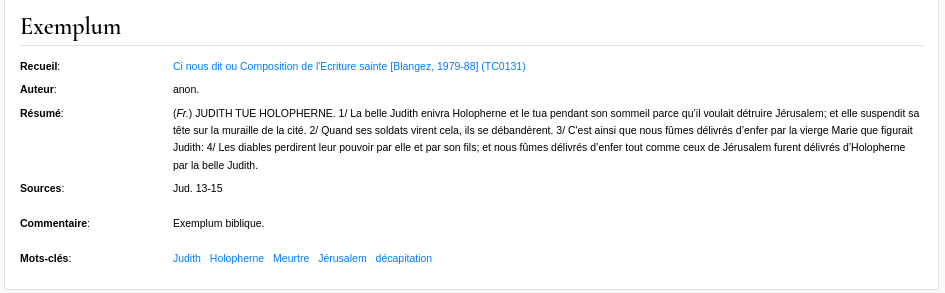
\includegraphics[width=0.8\linewidth]{images/jerusalemthema.png}}
		\caption{Mention de Jérusalem dans ThEMA}
	\end{figure}
	
	\begin{figure}[H]
		\centering
		\fbox{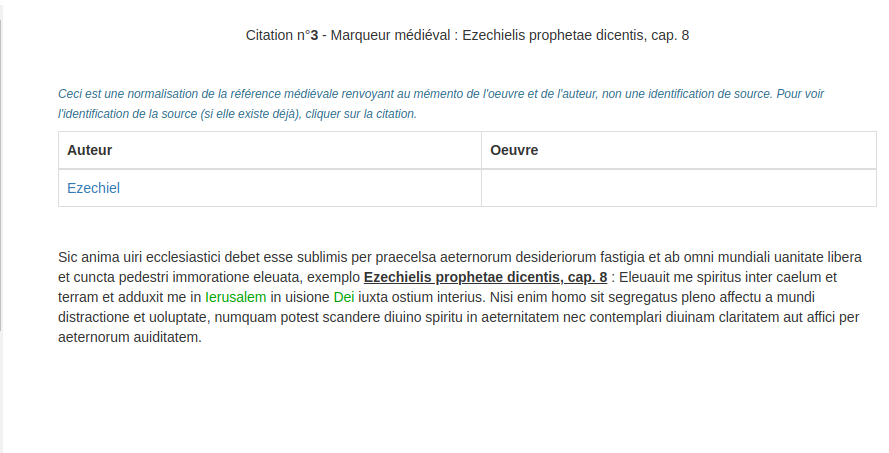
\includegraphics[width=0.6\linewidth]{images/mentionjerusalemsourcencyme.png}}
		\caption{Mention de Jérusalem dans SourcEncyMe}
	\end{figure}
	
\end{itemize}

Parmi les options de lien disponibles, j'ai décidé de me concentrer principalement sur les données. Cette décision repose sur plusieurs considérations : c’était un des objectifs principaux définis dans le livret de stage, et les utilisateurs s'intéressent principalement aux données, cherchant avant tout à accéder aux résumés de ThEMA et aux textes édités dans SourcEncyMe. Les \index{Mementos}mementos et les mots-clés, bien que facilitant les recherches thématiques, sont secondaires par rapport aux données essentielles pour la recherche historique. De plus, une \index{Encyclopédies}encyclopédie testée avait déjà fait l’objet d’un repérage préalable d’\textit{exempla} par une autre chercheuse de l’IRHT, Mara Calloni, et l’indexation des \index{Encyclopédies}encyclopédies dans ThEMA a facilité ce travail. 

En ce qui concerne les mots-clés, les noms de lieux et de personnes, le travail aurait été plus complexe, car SourcEncyMe n'a effectué qu'un repérage partiel à ce niveau dans les textes, contrairement à ThEMA. Quant aux liens vers les \index{Mementos}mementos, ils n'étaient pas prioritaires par rapport aux liens entre les textes, même s'ils auraient pu être établis assez facilement.


\section{Intégration des liens XML dans les bases de données}
Les textes des deux bases de données sont stockés dans des fichiers XML, ce qui a nécessité une réflexion sur l'insertion des liens et la recherche d'informations permettant de créer des liens. La gestion de ces liens a varié en fonction des spécificités de chaque base.

\subsection{Recherche des emplacements et des informations dans les XML pour la création des liens dans ThEMA}
Pour ThEMA, l'intégration des liens a été relativement simple. Les fichiers XML, un par \textit{exemplum}, comportaient déjà des balises spécifiques pour les liens, comme illustré dans l'exemple suivant : \\

\begin{lstlisting}[breaklines=true]
	<sourceDesc>
		<list type="source_details">
			<item type="source_text">
				<p/>
			</item>
			<item type="sources">
				<p/>
			</item>
			<item type="exemplum_context">
				<p>Feria quarta primae hebdomadae. Sermo I.</p>
			</item>
			<item type="commentary">
				<p/>
			</item>
			<item type="allegory">y</item>
		</list>
		<listBibl>
			<bibl type="manuscripts-editions" corresp="Z-IU7WR86C" n="t. I, p. 66-67"/>
		</listBibl>
		<list type="links">
			<item type="link" corresp="http://sermones.net/thesaurus/document.php?id=jvor_210">Sermones.net</item>
		</list>
		<list type="linked_exempla"/>
	</sourceDesc>
\end{lstlisting} 

\

\begin{figure}[H]
	\centering
	\fbox{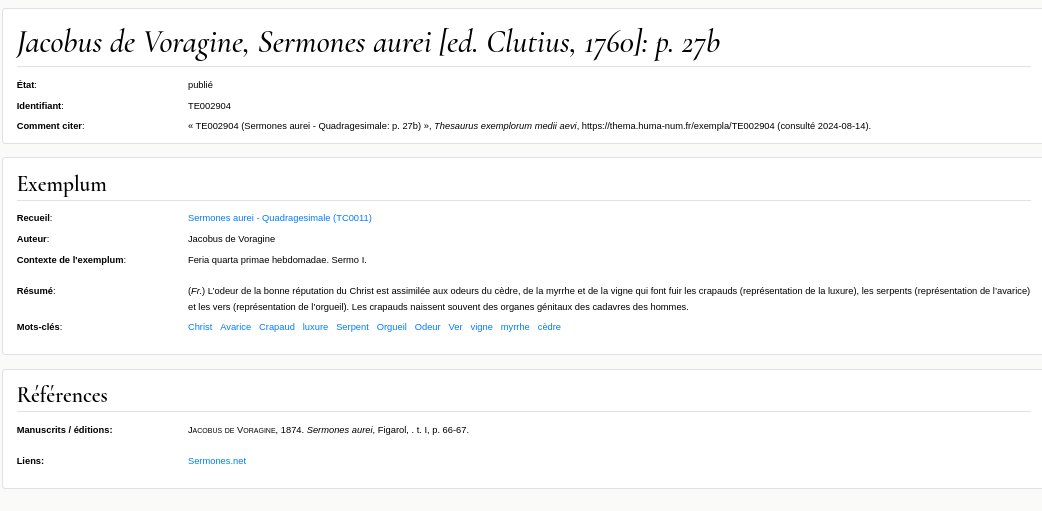
\includegraphics[width=0.8\linewidth]{images/exemplumaveclienthema.png}}
	\caption{Localisation du lien dans ThEMA}
\end{figure}

Les références aux \index{Encyclopédies}encyclopédies dans ThEMA se trouvent dans les champs « sources » et « textes apparentés ». Pour les récupérer, il faut naviguer dans les balises suivantes : <sourceDesc>, puis <list>, puis <item> avec l'attribut type="source", et enfin <p>. De même, pour les textes apparentés, il faut se rendre dans <sourceDesc>, puis <listBibl>, et enfin <bibl type="related\_texts"/>. \\

\

\begin{lstlisting}[breaklines=true]
	<sourceDesc>
		<list type="source_details">
			<item type="source_text">
				<p/>
			</item>
			<item type="sources">
				<p>Vincent de Beauvais, Speculum historiale, 13.50, dans Speculum quadruplex, vol. 4, 522a.</p>
			</item>
		<list>
	<sourceDesc>	
\end{lstlisting} 

\

\begin{lstlisting}[breaklines=true]
	</sourceDesc>
		<listBibl>
			<bibl type="related_texts" corresp="Z-E46747N6" n="p. 584"/>
			<bibl type="tubach" corresp="Z-WLZ7CBVC" n="TUB951"/>
		</listBibl>
		<list type="links"/>
		<list type="linked_exempla"/>
	</sourceDesc>
\end{lstlisting} 

\

\begin{figure}[H]
	\centering
	\fbox{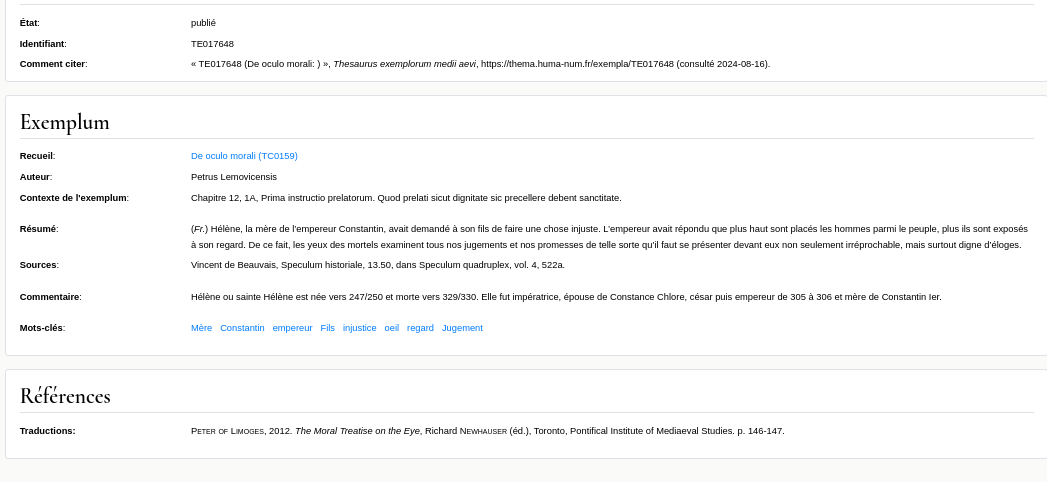
\includegraphics[width=0.8\linewidth]{images/vincentbeauvaisthema.png}}
	\caption{Champ source dans ThEMA}
\end{figure}

\subsection{Placement des liens et des visualisation des \textit{exempla} dans les XML de SourcEncyMe}

En revanche, dans SourcEncyMe, il n'existe pas de balises spécifiques pour intégrer les liens vers ThEMA. Chaque \index{Encyclopédies}encyclopédie est intégrée dans un fichier \index{XML}XML unique, comme montré dans l'annexe E. Initialement, j'avais envisagé d'ajouter de nouvelles balises <ref> avec un attribut spécifique pour les liens, en conformité avec les Tei Guidelines\footcite{17LinkingSegmentation}. Ce lien aurait été intégré dans la balise <cit> du XML, car dans SourcEncyMe, chaque citation d'un auteur est placée dans une balise <cit>. Voici la structure envisagée : \\

\begin{lstlisting}[breaklines=true]
<cit xml:id="cit_idp103803440">
	<bibl>
		<author ref="#gregorius_nazianzenus">Gregorius Nazianzenus</author>
	</bibl>
	<quote>Et hinc est quod venerabilis doctor<seg type="marqueur">Gregorius Nazianzenus</seg>cuius (testante<seg type="marqueur">Hieronymus</seg>) tanta auctoritas fuit&#160;: ut nullus unquam eius dictis calumniam inferre presumpserit&#160;: Immo insuper (ut testatur<seg type="marqueur">Rufinus</seg>) tanta fuit eius auctoritas apus ecclesias Christi, ut esse putaretur hereticus qui illi fuisset ausus in aliquo contraire. Hic itaque doctor hanc sibi consuetudinem fecerat, ut quicquid eius occurreret oculis de rebus exterioribus, interioribus anime moribus adaptaret&#160;: Sic enim refert ipse de se in suo apologetico, dicens&#160;: Mos mihi est ad meipsum singula queque revocare, precipue si quies mihi, sit, et silentium si vacet, animi moribus adaptare quod videtur in oculis. Unde et oculorum visio est mihi mentis eruditio. Huius igitur exemplum laudabile sequi oportet, si abundare volunt copia exemplorum. Que copia illis si affuerit, precipue de rebus extrinsecis que nobis sunt in aperto, et etiam de mirandis operibus que continue natura producit, vel adinvenit humana industria&#160;: non eos tantum apud curiosos auditores faciet gratiosos, quos mira nature opera vel humane inventionis studia narrata et patefacta delectant, sed etiam apud vulgus et simplices fructuosos et acceptos constituet, dum per exempla ad sensum spiritualia et subtilia declarabunt.
	</quote>
</cit>
\end{lstlisting}

Cependant, en plus de ce changement dans le XML, il aurait également fallu modifier le code de la base de données pour faire apparaître les liens. Cela aurait aussi posé problème car cela modifiait la structure globale du XML. Par conséquent, avec l’ingénieur de recherche Emmanuelle Khury, nous avons décidé d’intégrer les liens dans une balise préexistante pour éviter tout changement dans le XML. Nous avons choisi de placer le lien dans l’attribut correspondant de la balise <ref> qui se trouve dans la balise <bibl>. Cette dernière est utilisée dans SourcEncyMe pour indiquer une œuvre, comme vous pouvez le voir ici : \\

\begin{lstlisting}[breaklines=true]
	<cit n="2" xml:id="cit_id394697881596">
		<bibl>
			<ref target="#historiarum_adversum_paganos_orosii_libri_vii" type="oeuvre">Historiarum adversum paganos Orosii libri VII</ref>
			<author ref="#orosius_paulus">Orosius Paulus</author>
		</bibl>
		<bibl>
			<ref cert="low" corresp="https://thema.huma-num.fr/exempla/TE022184" target="#exemplum">Exemplum</ref>
		</bibl>
		<quote>
			<seg type="marqueur">Orosius de hormesta mundi libro primo</seg>Extant adhuc certissima monumenta gestorum. Nam tractus curruum et orbite rotarum, non solum in littore, sed etiam in profundo, nunc quousque visus admittitur pervidentur. Et si forte ad tempus casu vel curiositate conturbatur, mox divinitus in pristinam faciem ventis, fluctibusque reparantur, ut quisquis non docetur timore dei vel probate religionis studio, ita eius transacte ultionis terreatur <seg type="marqueur">exemplo.</seg>
		</quote>
	</cit>
\end{lstlisting}

\

De plus, un attribut cert="low" a été ajouté pour indiquer un faible taux de certitude, étant donné que l'ajout des liens a été automatisé\footnote{Il s'agissait de bien différencier les repérages faits de manière manuelle et ceux réalisés de manière automatique pour les chercheurs, dans un souci de transparence. Cette idée a été proposée par Emmanuelle Kuhry et Isabelle Draelants.}. De plus, si plusieurs liens sont présents, ils seront séparés par des espaces dans le même attribut corresp. Le lien sera visible car ce qui est inclus dans les balises <bibl> des balises <cit> est déjà affiché par le code de la base de données : \\

\begin{figure}[H]
	\centering
	\fbox{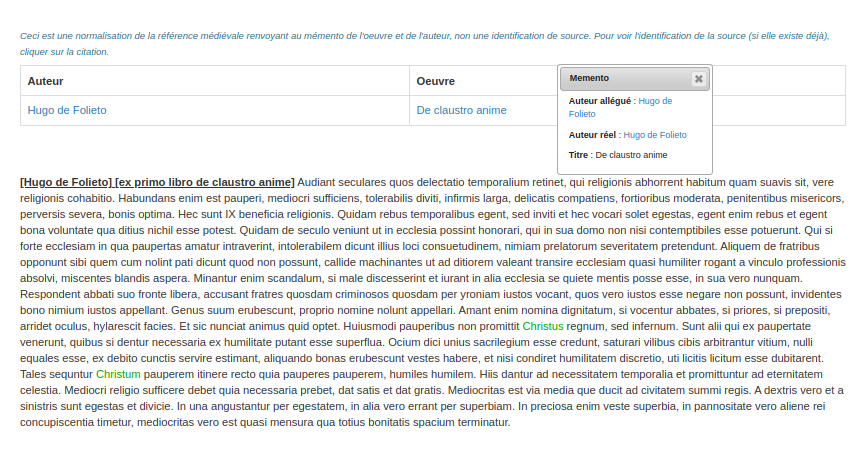
\includegraphics[width=0.7\linewidth]{images/affichagesourcencymeoeuvre.png}}
	\caption{Affichage de l'oeuvre dans SourcEncyMe}
\end{figure}

Enfin, pour indiquer la présence d'un \textit{exemplum} dans le texte, des marqueurs sont utilisés pour surligner le début du récit exemplaire ou son introduction (voir le code au-dessus). Bien que ces marqueurs soient normalement utilisés pour signaler le début d'une citation, ils ont été détournés de leur fonction initiale pour les \index{Récits exemplaires}récits exemplaires\footcite{SourcEncyMe}. Cependant, ces marqueurs ne sont présents que lorsque l'\textit{exemplum} est explicitement introduit, ce qui n'est pas toujours le cas.

\chapter{Repérages et recherches des données pour réaliser la connexion}
Avant de créer les liens entre les \textit{exempla} et les encyclopédies, il était essentiel d’identifier précisément les citations d'encyclopédies qui contiennent des \textit{exempla} et les récits exemplaires qui s'appuient sur ces \index{Encyclopédies}encyclopédies. Pour cela, j'ai ajouté un champ de recherche spécifique dans ThEMA et  un nom d'autorité a été ajouté dans SourcEncyMe par Emmanuelle Kuhry. J'ai également envisagé de comparer les textes entre ThEMA et SourcEncyMe pour repérer les réemplois d'encyclopédies dans SourcEncyMe et les \textit{exempla} dans ThEMA. En fin de compte, le repérage s'est principalement appuyé sur des mots-clés signalant les \textit{exempla} dans SourcEncyMe et sur la présence de mentions d'encyclopédies déjà indexées dans ThEMA.


\section{Création d'outils pour chercher dans les données qui seront connectées}
Pour faciliter l'accès des utilisateurs aux informations ayant aidé à faire des liens, des outils spécifiques dans les deux bases de données ont été mis en place.

\

Dans SourcEncyMe, tous les \textit{exempla} ont été catégorisés sous un même nom d'autorité (\textit{Exemplum}) par \index{Emmanuelle Kuhry}Emmanuelle Kuhry, même s'ils ne peuvent pas être entièrement considérés comme tels car chaque récits exemplaire peut être considéré comme œuvre à part entière\footnote{Cette autorité est désignée par un titre standardisé appelé entité canonique. \cite{SourcEncyMe}}. Ce choix a été guidé par des contraintes techniques : toutes les sources de la base sont balisées de manière uniforme, et pour éviter de créer un nouveau système de balisage, le balisage existant a été adapté pour inclure les \textit{exempla}. Ainsi, contrairement à ThEMA, où une distinction est faite entre différents types de récits, SourcEncyMe utilise le terme générique « exemplum » pour tous les \index{Récits exemplaires}récits exemplaires\footcite{InformationsThEMA}. \\

\begin{lstlisting}[breaklines=true]
	<cit xml:id="cit_idp94946128" n="11">
		<bibl>
			<ref target="#exemplum">Exemplum</ref>
		</bibl>
		<quote>Item activa vita assimilatur colli, primo, propter ordinem
		prioratus : est enim collis pes montis. Nam per collem ascendimus ad montem, quia scilicet per vitam activam ad contemplativam venimus. <name type="personne">Iacob</name> enim post <name type="personne">Lie</name> connubium (per quam activa vita signatur) ad <name type="personne">Rachaelis</name> pervenit amplexum, per quam contemplative vite formositas figuratur.</quote>
	</cit>
\end{lstlisting}

Grâce à ce système, les utilisateurs peuvent avec un champ de recherche spécifique, qui existait déjà avant mon stage, rechercher tous les \textit{exempla} présents dans les \index{Encyclopédies}encyclopédies en saisissant « exemplum » dans le champ « Œuvre » : \\

\begin{figure}[H]
	\centering
	\fbox{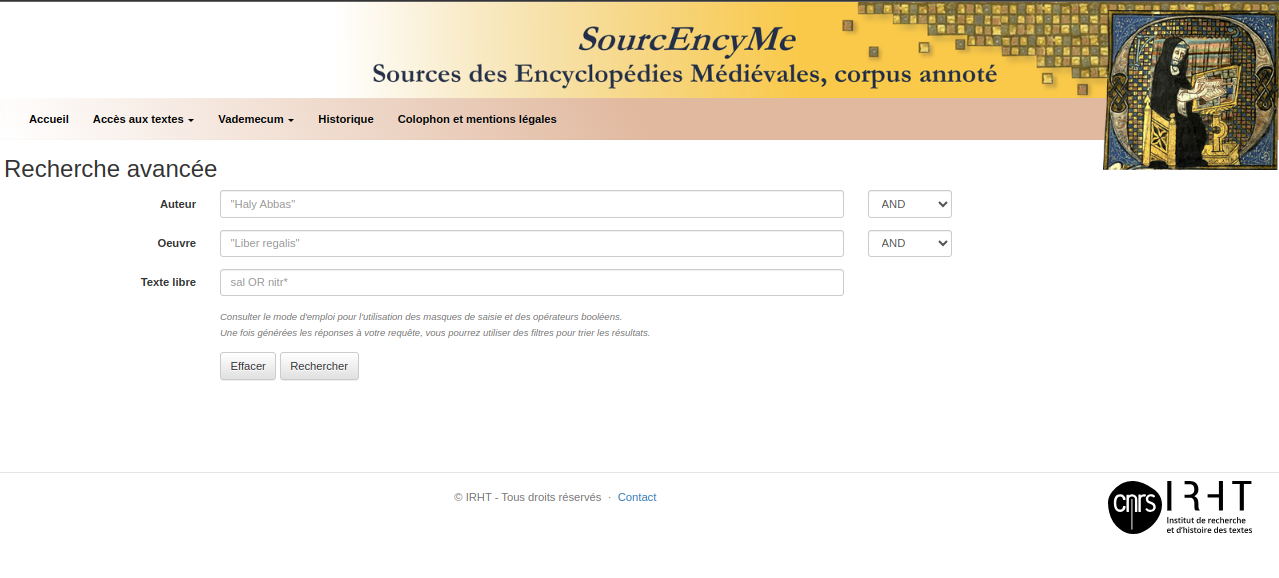
\includegraphics[width=0.8\linewidth]{images/champrecherchesourcencyme.png}}
	\caption{Champ de recherche dans SourcEncyMe}
\end{figure}

Dans ThEMA, en revanche, il a été nécessaire de créer un champ de recherche spécifique pour permettre aux utilisateurs d'explorer les sources et les textes apparentés. Bien que ces informations soient déjà visibles, il n'était pas possible de les rechercher directement. Pour remédier à cela, j'ai modifié le fichier « search.xql » situé dans le dossier « modules » de la base de données. J'ai adapté le code de recherche en texte intégral, initialement prévu pour les résumés des \index{Récits exemplaires}récits exemplaires, afin de permettre la recherche dans les sources et les textes apparentés (annexe F). \\

\begin{figure}[H]
	\centering
	\fbox{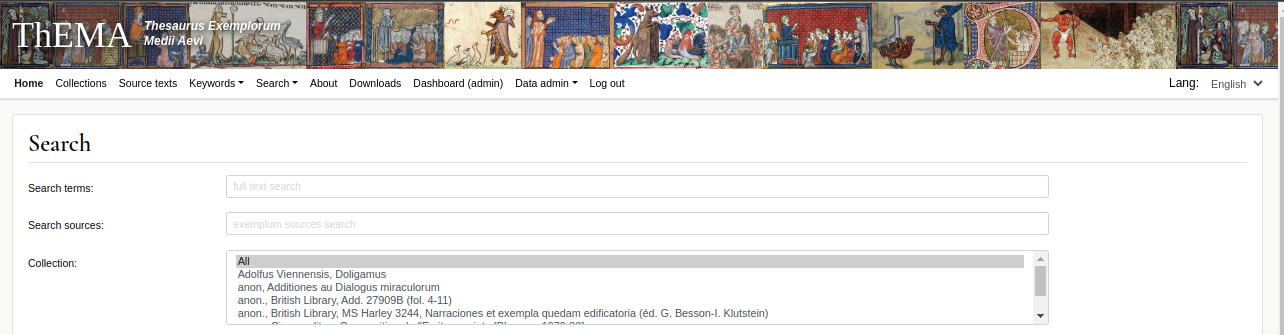
\includegraphics[width=0.8\linewidth]{images/champrecherchethemasource.png}}
	\caption{Nouveau champ de recherche dans ThEMA}
\end{figure}

Toutefois, le développement de ce code n'a pas pu être finalisé avant la fin de mon stage. En l'état, le code affiche l'ensemble des \textit{exempla} en haut de la page ainsi que les résultats de recherche dans les sources et textes apparentés en bas, alors qu'il aurait dû se limiter à afficher uniquement ces derniers. \\

\begin{figure}[H]
	\centering
	\fbox{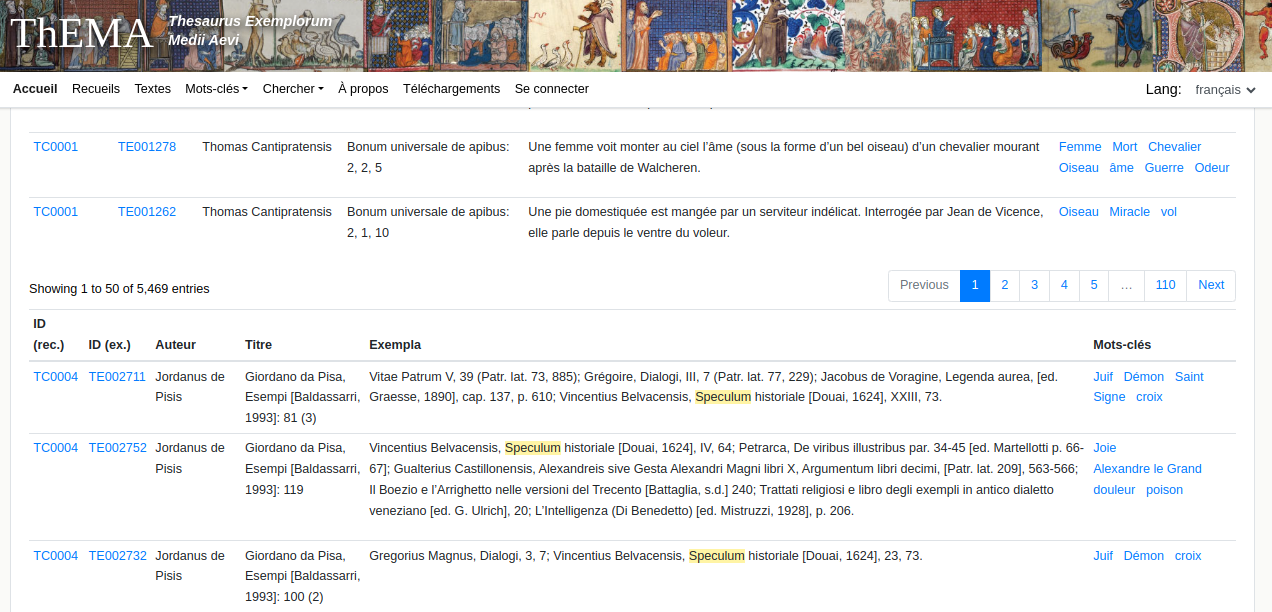
\includegraphics[width=0.8\linewidth]{images/pugthema.png}}
	\caption{Résultat du nouveau champ de recherche dans ThEMA}
\end{figure}

\section{Identification des liens par comparaison des textes}
Après avoir mis en place ces outils pour faciliter la recherche d'\textit{exempla}` et d'\index{Encyclopédies}encyclopédies dans ThEMA et SourcEncyMe, j'ai également exploré la possibilité d'utiliser des méthodes plus avancées pour affiner encore davantage cette analyse et trouver des liens qui n'ont pas encore été repérés. C'est ainsi que j'ai envisagé l'utilisation de l'intelligence artificielle pour comparer les textes des deux bases de données. L'idée était de tirer parti de la rapidité et de la précision de l'IA pour détecter non seulement les \textit{exempla} dans SourcEncyMe, mais aussi pour identifier des mentions d'encyclopédies supplémentaires dans ThEMA, au-delà de celles déjà repérées lors de l'indexation initiale.

Toutefois, cette approche s'est rapidement heurtée à plusieurs défis. Le premier obstacle provenait d'une différence importante entre les deux bases de données. ThEMA, pour des raisons de droits d'auteur, ne peut fournir que de courts résumés en français des \index{Récits exemplaires}récits exemplaires, tandis que SourcEncyMe donne accès aux textes complets en latin, car des éditions récentes n'existent pas forcément. Cette disparité linguistique a rendu l'utilisation de l'intelligence artificielle complexe, nécessitant la traduction des textes des \index{Encyclopédies}encyclopédies en français pour permettre une comparaison efficace\footnote{Je n'ai pas trouvé de modèles de langues entraînés pour le latin. De toute manière, ThEMA ne possèdent qu'un nombre limité de récits où le texte latin et indiqué}.\\

\begin{figure}[H]
	\centering
	\fbox{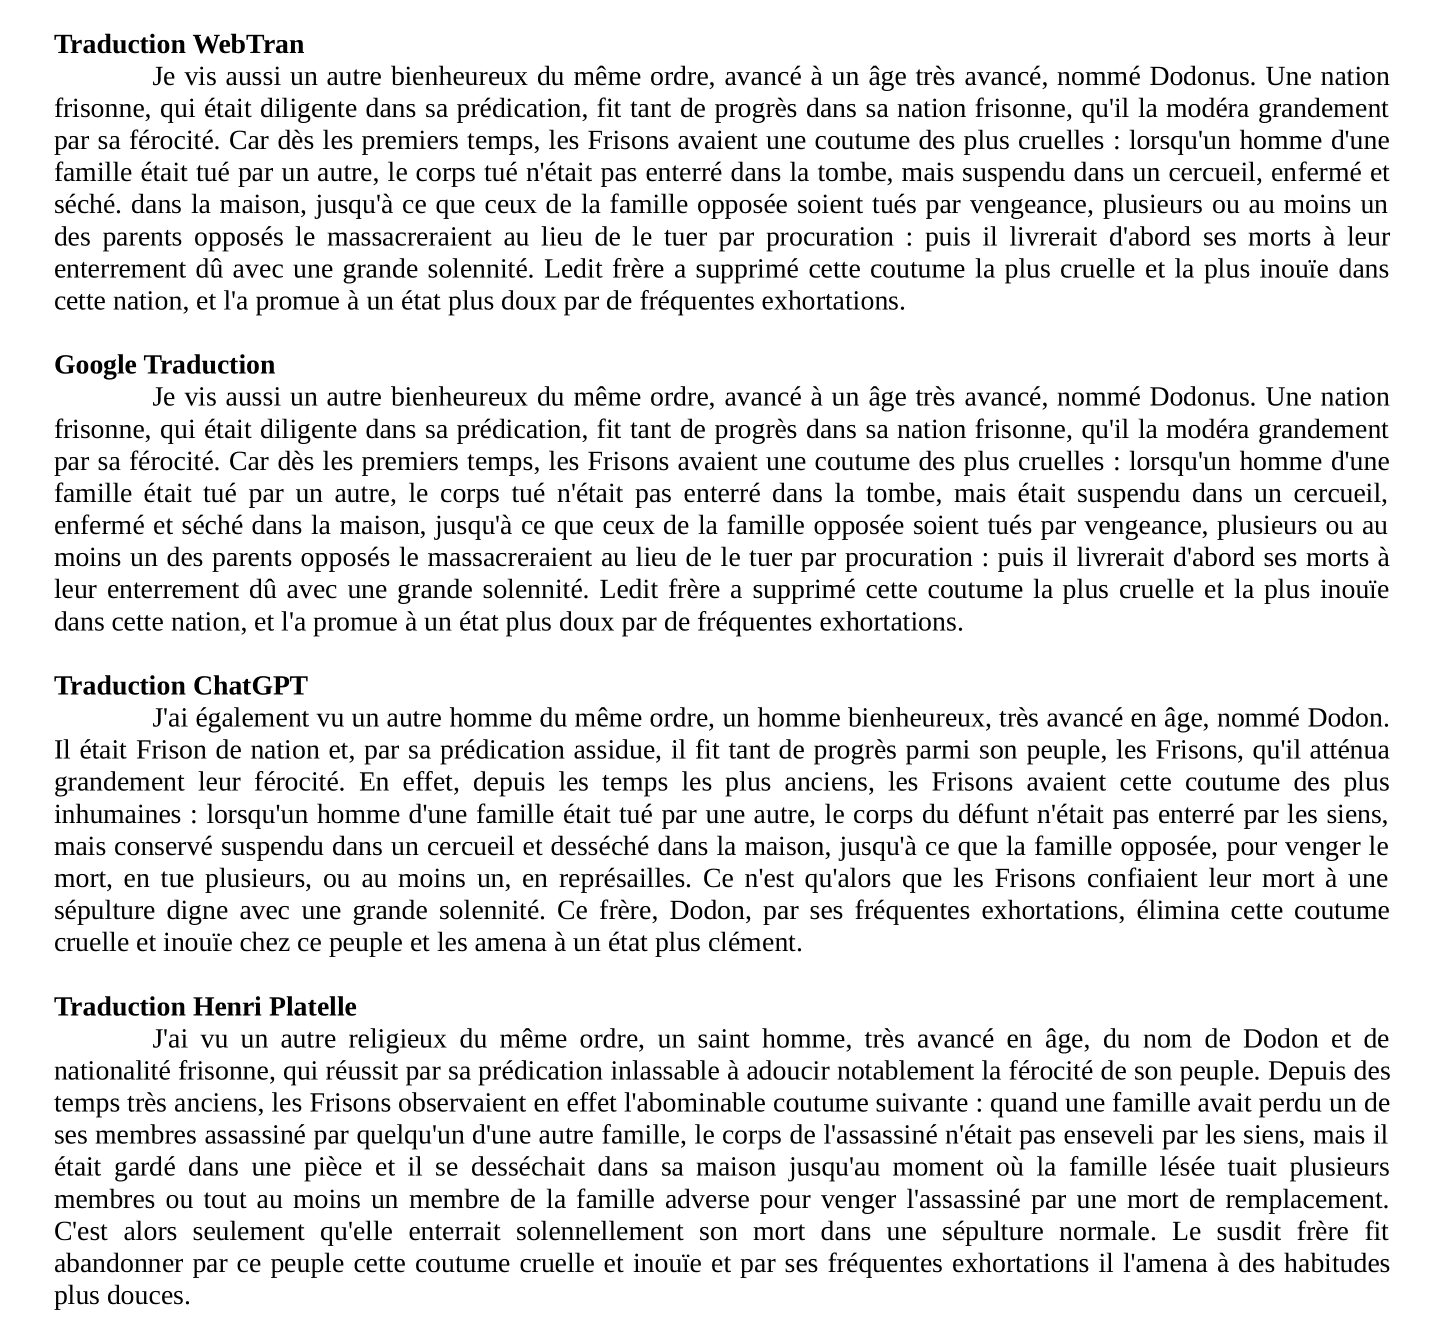
\includegraphics[width=0.8\linewidth]{images/tradlang.png}}
	\caption{Différentes traductions d'un même \textit{exemplum}}
\end{figure} 

La traduction elle-même a posé des problèmes. Malgré plusieurs tentatives, je n'ai trouvé aucun traducteur en ligne parfaitement fiable. Parmi les outils testés, ChatGPT se distinguait légèrement de Google Traduction et de WebTran, mais ces outils imposaient des restrictions sur le web scraping, la technique d'extraction automatisée de données à partir de sites web. Pour ChatGPT, l'achat de jetons était requis pour accomplir cette tâche, tandis que Google Traduction et WebTran interdisaient explicitement le web scraping dans leurs conditions d'utilisation, compliquant encore davantage le processus.

En fin de compte, la solution retenue a été de traduire manuellement, ou partiellement, les textes des \index{Encyclopédies}encyclopédies en m'appuyant sur des ressources en ligne. Bien que la traduction reste imparfaite, un code que j'ai développé (annexe G) a permis de repérer certaines similitudes entre les textes. Cependant, même avec des optimisations, ce traitement s'est révélé extrêmement lent : chaque comparaison prenait environ 20 minutes, en raison du volume important de données à analyser.

\

Le code, bien qu'imparfait, s'est montré relativement efficace. Lors d'un test visant à trouver les nombreuses équivalences de l'\textit{exemplum} de la « moniale chaste mais bavarde »\footcite{RecitsExemplairesMoniale}, le code a réussi à identifier le texte utilisé pour la recherche avec une précision de 100 \%, et les autres textes similaires se sont classés en tête des pourcentages de similarité :

\begin{figure}[H]
	\centering
	\fbox{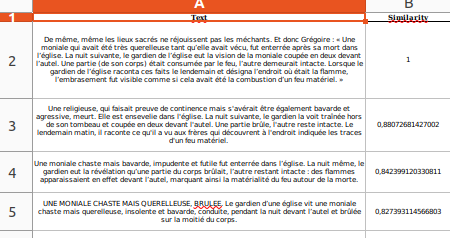
\includegraphics[width=0.7\linewidth]{images/similarite1.png}}
	\caption{Essai de comparaison}
\end{figure}

Malgré ces résultats encourageants, j'ai finalement décidé de renoncer à l'utilisation de l'IA pour trouver des correspondances entre les textes des deux bases de données. Cette décision s'explique par les nombreuses limitations rencontrées, notamment les problèmes de traduction, la lenteur des analyses, et la difficulté à définir ce qu'est un \textit{exemplum} : une forme littéraire complexe et fluide, difficile à cerner tant par un humain que par un algorithme\footcite{berliozIntroductionGenerale2010}. De plus, les \textit{exempla} présents dans les \index{Encyclopédies}encyclopédies diffèrent souvent de ceux répertoriés dans ThEMA, rendant la tâche encore plus ardue pour une IA. Un exemple illustrant cette difficulté est un \textit{exemplum} retrouvé dans la \textit{Summa de exemplis ac similitudinibus rerum} de Giovanni da San Gimignano, où l'auteur reprend une idée d'Aristote sur la nécessité de cultiver son cœur pour produire de bons fruits\footcite{RecitExemplaireUtilise}. Ce récit n'a trouvé aucun équivalent exact dans le corpus de ThEMA, le texte le plus proche présentant seulement 70\% de similarité. \\

\begin{figure}[H]
	\centering
	\fbox{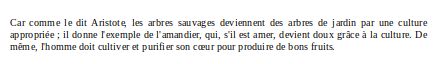
\includegraphics[width=0.8\linewidth]{images/textrecherche.png}}
	\caption{\textit{Exemplum} repéré dans SourcEncyMe}
\end{figure}

\begin{figure}[H]
	\centering
	\fbox{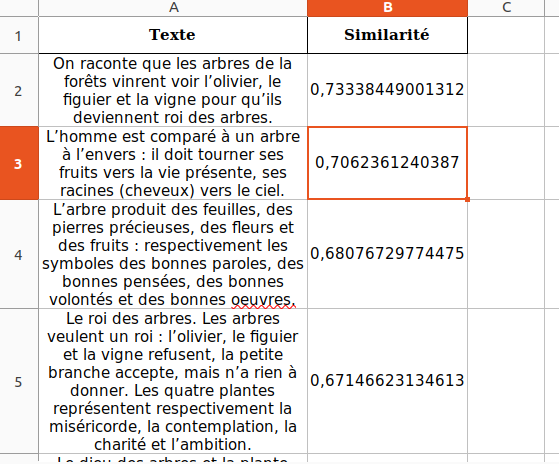
\includegraphics[width=0.6\linewidth]{images/similitude2.png}}
	\caption{Comparaison de l'\textit{exemplum} avec les récits exemplaire de ThEMA}
\end{figure}

Ainsi, j'ai préféré adopter une approche plus simple : repérer semi-manuellement les \textit{exempla} dans les encyclopédies. Contrairement à ThEMA, où les liens avec les encyclopédies ont été établis lors de l'indexation, ces \textit{exempla} n'ont pas encore été identifiés dans les \index{Encyclopédies}encyclopédies. L'entraînement d'un modèle de langage pour reconnaître un \textit{exemplum} aurait été une solution intéressante, mais il aurait fallu surmonter à nouveau les défis précédemment présentés.


\section{Identification des \textit{exempla} via des mots-clés}
Face à ces défis, il est apparu que l'utilisation d'une méthode plus ciblée pourrait s'avérer plus efficace. C'est ainsi que j'ai opté pour l'application de mots clés spécifiques. Cette méthode repose sur une caractéristique fréquente des \index{Récits exemplaires}récits exemplaires : ils sont souvent introduits par des termes latins comme « audivi », « legi », « memini », « verum », « dicitur », « narrat », « memini » ou « vidi »\footcite{bremondclaudeExemplum1982}. Cependant, tous ces mots n'ont pas été retenus, car dans les œuvres encyclopédiques, ils sont souvent utilisés dans d'autres contextes, notamment pour citer des œuvres ou des auteurs.

Par conséquent, je me suis concentré sur les mots les plus directement liés aux \textit{exempla} : « exemplum », « exempla », « exemplo », et « exemplis ». Cette approche par mots-clés m'a permis de contourner les difficultés liées à l'intelligence artificielle tout en offrant une méthode efficace pour identifier les \textit{exempla} dans les textes encyclopédiques.

De ce fait, avec une feuille de style \index{XSL}XSL, c'est-à-dire une page de code utilisée pour transformer et présenter des documents \index{XML}XML, j'ai créé un code qui, lorsqu'il rencontre l'une des déclinaisons d'\textit{exemplum} dans la balise <quote> du \index{XML}XML (c'est-à-dire là où se trouve le texte), balise le mot avec un marqueur et crée ensuite une balise <bibl>, si nécessaire, au-dessus de <quote> pour indiquer qu'il y a un \textit{exemplum}. Voilà ce que fait la transformation : \\

\begin{lstlisting}[breaklines=true]
	<cit n="7" xml:id="cit_idp82718352">
		<quote>Sexto, quia malus seruus cupidus existens, bona Domini in proprium usum vertit. Exemplum de seruo <name type="personne">Elisei</name>, et hoc pertinet ad simoniacos, qui bona Domini, id est,dona Spiritus sancti, pro sua utilitate temporali emunt, et vendunt.
		</quote>
	</cit>
\end{lstlisting}

\

\begin{lstlisting}[breaklines=true]
	<cit n="7" xml:id="cit_idp82718352">
		<bibl>
			<ref cert="low" target="#exemplum">Exemplum</ref>
		</bibl>
		<quote>Sexto, quia malus seruus cupidus existens, bona Domini in proprium usum vertit. <seg type="marqueur">Exemplum</seg> de seruo <name type="personne">Elisei</name>, et hoc pertinet ad simoniacos, qui bona Domini, id est, dona Spiritus sancti, pro sua utilitate temporali emunt, et vendunt.
		</quote>
	</cit>
\end{lstlisting}

\

Au départ, je souhaitais que ce code fonctionne uniquement lorsque les déclinaisons du mot « exemplum » se trouvent en début de phrase, car j'avais remarqué que c'est souvent dans ces cas-là que l'on a affaire à un véritable \textit{exemplum}. Cependant, après discussion avec \index{Isabelle Draelants}Isabelle Draelants et \index{Emmanuelle Kuhry}Emmanuelle Kuhry, cette approche a été abandonnée car elle risquait de laisser de côté certains récits exemplaires. Le choix a été fait d'effectuer un repérage plus large, quitte à avoir plus d'erreurs (annexe H), ce qui a nécessité un travail de vérification.

Prenons l'exemple de l'\index{Encyclopédies}encyclopédie de Giovanni da San Gimignano. Mara Calloni avait initialement identifié 220 \textit{exempla} en lisant le texte. Le code, pour sa part, en a détecté plus de 650. Après vérification par mes soins, le nombre exact d'\textit{exempla} est de 479. Bien que ce chiffre puisse sembler élevé, il est important de noter que l'ensemble de l'œuvre encyclopédique de San Gimignano est moralisée\footcite{oldoniGiovanniSanGimignano1994}. Le code repère donc un plus grand nombre d'\textit{exempla} que la lecture humaine, mais il se concentre uniquement sur les déclinaisons du mot \textit{exemplum}. En revanche, le repérage manuel effectué par Mara, qui ne faisait aucune discrimination dans les citations, a permis de déceler des \textit{exempla} même lorsqu'ils ne sont pas explicitement introduits par ces déclinaisons. Toutefois, l'ajout de mots introductifs supplémentaires pour affiner la recherche augmenterait considérablement la charge de travail pour la vérification, qui prenait déjà une quinzaine d'heures rien que pour les déclinaisons du mot \textit{exemplum}. Il est donc essentiel de déterminer jusqu'où nous sommes prêts à aller dans ce processus de vérification, car autrement, cela reviendrait presque à effectuer une recherche par lecture. Cela dit, cette méthode facilite le balisage, puisqu'il suffit ensuite de supprimer les éléments qui ne correspondent pas à un \textit{exemplum}.

C'est surtout avec le mot \textit{exemplum} que le plus grand nombre de \index{Récits exemplaires}récits exemplaires ont été trouvés (140), suivi par \textit{exemplo} (30), \textit{exempla} (13) et \textit{exemplis} (5). Cette répartition s'explique aisément. \textit{Exemplum} (nominatif singulier) est la forme de base du mot en latin\footcite{PageDedieeAu2024}. Elle est souvent utilisée pour introduire un récit exemplaire en tant que concept ou titre. \textit{Exemplo} (ablatif ou datif singulier) est fréquemment utilisé dans les constructions syntaxiques pour indiquer le moyen ou la cause (par exemple, « par un exemple », « grâce à l'exemple de... »)\footcite{PageDedieeAu2024}. Cette forme est souvent intégrée dans des phrases qui illustrent ou justifient un point par l'utilisation d'un exemple, ce qui la rend très présente dans les textes qui visent à enseigner ou moraliser. %Input: importer un fichier

\chapter{Création des liens dans les bases de données}	%etc.
fAprès avoir identifié les \textit{exempla} dans SourcEncyMe et les encyclopédies dans ThEMA, il a été nécessaire de créer des connexions entre les deux bases de données. Pour ce faire, j’ai d'abord indexé les \textit{exempla} identifiés dans SourcEncyMe en les regroupant dans un recueil factice où les liens pouvaient être ajoutés. Ensuite, j'ai développé un code permettant d'ajouter des liens vers les \textit{exempla} qui contiennent des références à des \index{Encyclopédies}encyclopédies.


\section{Indexation des \textit{exempla} de SourcEncyMe dans ThEMA}
Une fois les \index{Récits exemplaires}récits exemplaires repérés dans SourcEncyMe, il était essentiel de les connecter à ThEMA. La question s’est posée de savoir où et comment les placer dans la base de données. L'équipe de SourcEncyMe envisageait de créer des entrées d’\textit{exempla} directement dans ThEMA en y ajoutant les informations pertinentes. Cependant, cette approche ne correspondait pas au fonctionnement de ThEMA, où les \textit{exempla} sont toujours intégrés dans un recueil spécifique, respectant ainsi le contexte et l’auteur d'origine.

Avec l'accord d'\index{Isabelle Draelants}Isabelle Draelants et de \index{Marie-Anne Polo de Beaulieu}Marie-Anne Polo de Beaulieu, nous avons décidé de créer un recueil intitulé « \textit{Exempla} de [Nom de l'encyclopédie] ». Cette solution s'inscrivait dans la vision de ThEMA, qui se veut une base de données d’œuvres contenant des \textit{exempla}, sans se limiter aux seuls recueils d'\textit{exempla}. De plus, lors de l'indexation, nous avons choisi d’inclure un extrait du texte en latin de l'\textit{exemplum} trouvé dans l'encyclopédie dans le champ : « texte original ». Cependant, étant donné que le texte des \index{Encyclopédies}encyclopédies est encore en cours de révision, il a été convenu que ces extraits seraient éventuellement supprimés pour éviter la diffusion de versions incorrectes. À l'avenir, des chercheurs ou des étudiants seront chargés de finaliser l'indexation en créant des résumés et en ajoutant des mots-clés, après quoi les extraits en latin seront retirés. L'indexateur pourra également supprimer un \textit{exemplum} s'il estime qu'il n'en est pas véritablement un, car il ne faut pas oublier qu'une partie des \textit{exempla} a été identifiée automatiquement par un algorithme. Dans ce cas, il devra simplement contacter l'équipe de SourcEncyMe pour qu'ils mettent à jour le lien de leur côté.

Pour intégrer les \textit{exempla} dans ThEMA, j'avais initialement envisagé d’utiliser un code \index{Python}Python ou \index{XQuery}XQuery pour générer les fichiers \index{XML}XML des \textit{exempla}. Ils auraient recréé le schéma \index{XML}XML des \textit{exempla} de ThEMA et il aurait juste fallu réintégrer les XML des \index{Récits exemplaires}récits exemplaires dans la base pour qu'ils apparaissent. Mais j’ai finalement opté pour une solution différente. J’ai développé un script \index{Python}Python de web scraping (annexe I) qui tire parti de l'interface de création d'\textit{exempla} déjà existante dans la base de données. Ce script se connecte à la base de données locale, navigue dans le recueil créé, crée chaque \textit{exemplum}, y insère le texte source, et répète l’opération pour chaque \textit{exemplum} repéré.  Le code cible plus spécifiquement toute les <ref', target="\#exemplum"> et récupère le texte dans la balise <quote> en dessous. Le code ne cible par le marqueur \textit{exemplum} car il n'est pas toujours présent même si un \textit{exemplum} est dans le texte. Cette méthode a l’avantage de créer directement les \textit{exempla} dans la base, sans avoir à charger manuellement les fichiers XML, réduisant ainsi les risques d'erreurs.

Ce code pourra être réutilisé à l'avenir pour accélérer l'indexation des textes dans ThEMA, à condition que les \textit{exempla} soient préalablement balisés. Il pourrait également être amélioré en intégrant un module capable de générer automatiquement des mots-clés pour les résumés, ce qui rendrait le processus d'indexation encore plus rapide.


\section{Gestion des liens vers SourcEncyMe dans ThEMA}
\subsection{Création des liens}
Lors de l'intégration des liens dans mon code, j'ai rencontré un problème. Le créateur d'\textit{exempla} de la base ThEMA possède un champ spécifique pour ajouter ces liens, mais ce champ est « dynamique ». Cela signifie que la page peut se modifier ou réagir aux actions de l'utilisateur sans nécessiter un rechargement complet. Cependant, mon code ne parvenait pas à interagir correctement avec cette partie dynamique, qui permet d'ajouter ou de supprimer des liens. \\
 
 \begin{figure}[H]
 	\centering
 	\fbox{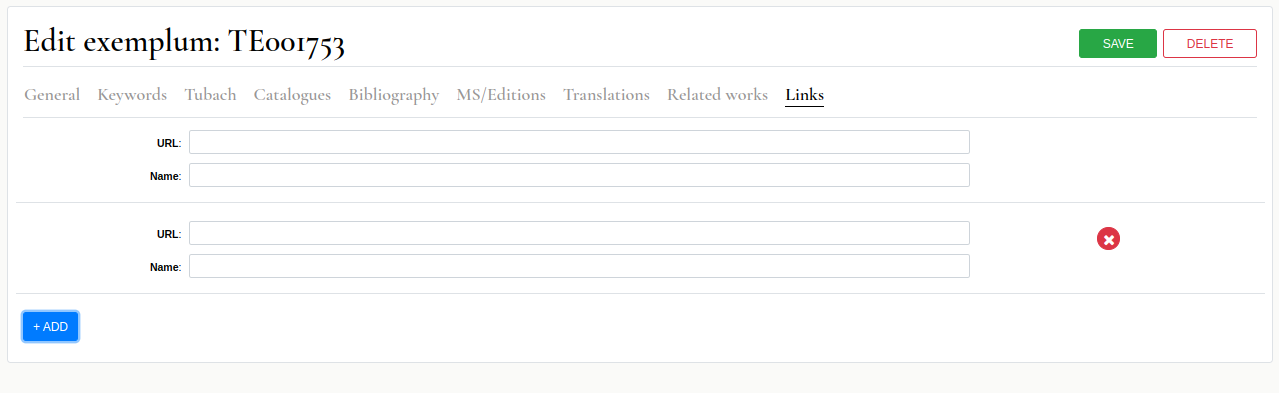
\includegraphics[width=0.5\linewidth]{images/champlienthema.png}}
 	\caption{Page dynamique pour ajouter des liens dans ThEMA}
 \end{figure}

Finalement, il a été nécessaire de développer un script \index{Python}Python pour modifier les fichiers XML et y ajouter les liens (annexe J). Pour cela, j'ai dû télécharger le dossier contenant les \textit{exempla} de Giovanni da San Gimignano. Le script vérifie d'abord que le texte dans les \index{XML}XML de ThEMA correspond bien à celui dans SourcEncyMe. Une fois cette vérification effectuée, le lien vers SourcEncyMe est ajouté dans les \index{XML}XML de ThEMA, et dans les \index{XML}XML de SourcEncyMe. Les liens sont construits comme suit : \\

 \begin{figure}[H]
	\centering
	\fbox{
\includegraphics[width=0.8\linewidth]{images/lienthemaexemple.png}}
	\caption{Exemple de lien vers ThEMA}
\end{figure}

Pour accéder aux exempla, la base ThEMA passe d'abord par Huma-Num qui héberge la base. Ensuite, elle interroge le fichier « exempla.xql » pour afficher les \textit{exempla} sous forme de contenu web. Enfin, elle appelle le fichier \index{XML}XML correspondant à l'\textit{exemplum} créé dans ThEMA. \\

\begin{figure}[H]
	\centering
	\fbox{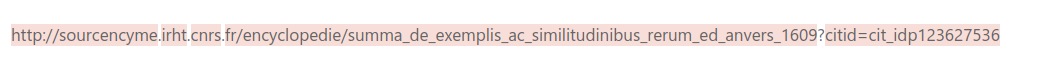
\includegraphics[width=0.8\linewidth]{images/linksourcencymeexemple.png}}
	\caption{Exemple de lien vers SourcEncyMe}
\end{figure}

Pour accéder aux citations d'\index{Encyclopédies}encyclopédies, la base SourcEncyMe passe par l'IRHT et le CNRS, qui hébergent la base de données. Ensuite, elle interroge le fichier gérant les encyclopédies et leur affichage web. Enfin, elle appelle une encyclopédie spécifique et une citation précise identifiée par un code cit\_id, unique pour chaque citation, trouvé dans la balise <cit> : \\

 \begin{figure}[H]
	\centering
	\fbox{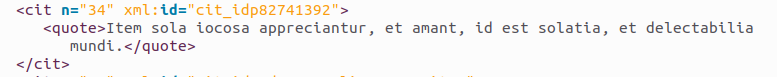
\includegraphics[width=0.8\linewidth]{images/citidsourcenycme.png}}
	\caption{Localisation du cit\_id dans SourcEncyMe}
\end{figure}

Avant de créer les liens, j'ai vérifié auprès des deux équipes si les identifiants resteraient constants dans le temps pour garantir la pérennité des liens.


\subsection{Perspectives pour la création du lien}
Dans une perspective d'amélioration future, j'ai envisagé de modifier le champ d'ajout de liens pour qu'il fonctionne de manière similaire aux autres champs contenant des données préenregistrées. L'objectif serait de préenregistrer tous les liens vers SourcEncyMe, afin d'éviter aux chercheurs de les copier manuellement et de supprimer la nécessité de modifier directement les fichiers \index{XML}XML à l'aide d'un script \index{Python}Python.

J'avais envisagé d'apporter des modifications à l'interface de balisage XMLmind, utilisée pour baliser les \index{Encyclopédies}encyclopédies de SourcEncyMe. Cependant, je n'ai pas eu le temps de m'en occuper, et c'est finalement \index{Emmanuelle Kuhry}Emmanuelle Kuhry qui s'est proposée de s'en charger. Il sera nécessaire d'adapter la fenêtre pop-up permettant de sélectionner une œuvre pour une citation dans XMLmind, en y ajoutant des liens vers les \textit{exempla} de la base et la classification de Tubach.


\section{Création de liens vers SourcEncyMe depuis les mentions d'encyclopédies dans ThEMA}
Pour ajouter des liens entre les \textit{exempla} et les références à des \index{Encyclopédies}encyclopédies, j'ai utilisé un script \index{Python}Python (annexe K) qui explore les fichiers \index{XML}XML de la base téléchargée sur mon ordinateur. Le script recherche des mentions d'encyclopédies en utilisant une expression régulière spécifiée pour chaque encyclopédie. Par exemple, pour le \index{Speculum historiale}\textit{Speculum historiale}, l'expression régulière utilisée est : \\

\begin{verbatim} r'S?s?peculum historiale,? ([IVXLCDM]+|\d+)[.,]?\s*([0-9]+)?' \end{verbatim}

\

Cette expression régulière est conçue pour détecter les références au texte \index{Speculum historiale}\textit{Speculum historiale}, en tenant compte des variations possibles dans l'usage des majuscules, ainsi que des numéros de volume en chiffres romains ou arabes. Le script continue en récupérant les numéros de chapitre mentionnés et en cherchant ces numéros dans le fichier \index{XML}XML de l'\index{Encyclopédies}encyclopédie. Une fois le numéro de chapitre trouvé, il est converti en chiffre arabe si nécessaire. Le script récupère ensuite le cit\_id correspondant et l'insère dans un lien préétabli au nom de l'encyclopédie (à ajuster par l'utilisateur), puis intègre ce lien dans le \index{XML}XML de ThEMA. Finalement, le script place l'identifiant TE... dans le champ cit du \index{XML}XML, car il s'agit d'un élément repris et non d'un \textit{exemplum}, ce qui évite l'identification d'une œuvre.

Cependant, plusieurs problèmes ont été rencontrés lors de l'exécution de ce code. Premièrement, l'extraction des mentions d'\index{Encyclopédies}encyclopédies s'est révélée compliquée en raison de l'utilisation mixte d'indexations en texte intégral et d'attributs récupérés lors du chargement de la page web de la base de données. Les attributs spécifiques associés aux encyclopédies, stockés dans le fichier list\_bibliography.xml, sont : \\

\begin{center}
\begin{tabular}{|c|c|}
	\hline
	Z-S7UCXT48 & \index{Speculum naturale}\textit{Speculum naturale} \\
	\hline
	Z-38N6WX3E & \index{Speculum historiale}\textit{Speculum historiale}  \\
	\hline
	Z-D6KRQBMP & \textit{Liber de natura rerum} \\
	\hline
\end{tabular}
\end{center}

\

Le script devait donc non seulement effectuer des recherches en texte intégral mais aussi intégrer et traduire ces codes avant de réaliser les recherches en texte intégral. Voilà à quoi ressemble un cas de mention plein texte d'encyclopédie dans un XML de ThEMA et une mention d'encyclopédie liée à un attribut : \\

\begin{lstlisting}[breaklines=true]
<sourceDesc>
	<list type="source_details">
		<item type="source_text"><p/></item>
		<item type="sources"><p>Vincent de Beauvais, Speculum naturale, 16, 97 (Douai, 1624, col. 1213).</p></item>
		<item type="exemplum_context"><p>III, tit. VI, De peregrinatione</p></item>
		<item type="commentary"><p/></item>
		<item type="allegory">n</item>
	</list>
\end{lstlisting}

\begin{lstlisting}[breaklines=true]
<listBibl>
	<bibl type="tubach" corresp="Z-WLZ7CBVC" n="TUB3969"/>
	<bibl type="related_texts" corresp="" n="">Valerius Maximus, Dictorum factorumque memorabilium libri novem..., V, c.4.7.ext.</bibl>
	<bibl type="related_texts" corresp="Z-38N6WX3E" n="6, 125"/>
	<bibl type="related_texts" corresp="" n="">British Library, Add. 33956 [transcr. Welter], 427</bibl>
	<bibl type="related_texts" corresp="" n="">Liber ad status [Paris, BnF, ms. lat. 6368], 4,21</bibl>
\end{lstlisting}

\begin{lstlisting}[breaklines=true]
<biblStruct xml:id="Z-38N6WX3E" type="book" corresp="#http://zotero.org/groups/2304628/items/38N6WX3E">
	<monogr>
		<title level="monograph">Speculum historiale</title>
		<title level="short"/>
		<author>
			<name>Vincentius Belvacensis</name>
		</author>
		<imprint>
			<pubPlace>Douai</pubPlace>
			<date type="pub_date">1624</date>
		</imprint>
	</monogr>
</biblStruct>
\end{lstlisting}

\

Un autre problème rencontré concernait la différence entre les numéros de chapitres indexés dans ThEMA et ceux présents dans SourcEncyMe. Les numéros de chapitres utilisés par les indexateurs pour le \textit{Speculum historiale} sont basés sur l'édition de 1624, tandis que le classement de SourcEncyMe est décalé d'un numéro\footnote{Vincent de Beauvais, \textit{Speculum historiale}. \textit{Bibliotheca mundi Vincentii Burgundi, ex ordine Praedicatorum venerabilis episcopi Bellovacensis, Speculum quadruplex, naturale, doctrinale, morale, historiale}, Douai, ex officina typographica Baltazaris Belleri, 1624.}. Ainsi, chaque fois que le code récupère un numéro de chapitre de ThEMA, il doit ajouter un à ce numéro pour correspondre à SourcEncyMe. Par exemple, pour l'\textit{exemplum} 844 de la \textit{Scala Coeli}, les indexateurs ont mentionné le chapitre 26, 32, alors que dans SourcEncyMe, ce textes se trouve au chapitre 27, 33. \\

 \begin{figure}[H]
	\centering
	\fbox{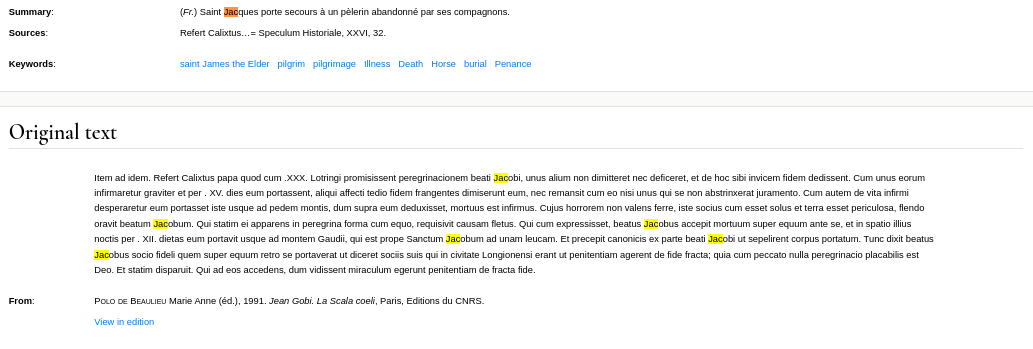
\includegraphics[width=0.8\linewidth]{images/problemnumero1.png}}
	\caption{Récit exemplaire reprenant un texte encyclopédique}
\end{figure}

 \begin{figure}[H]
	\centering
	\fbox{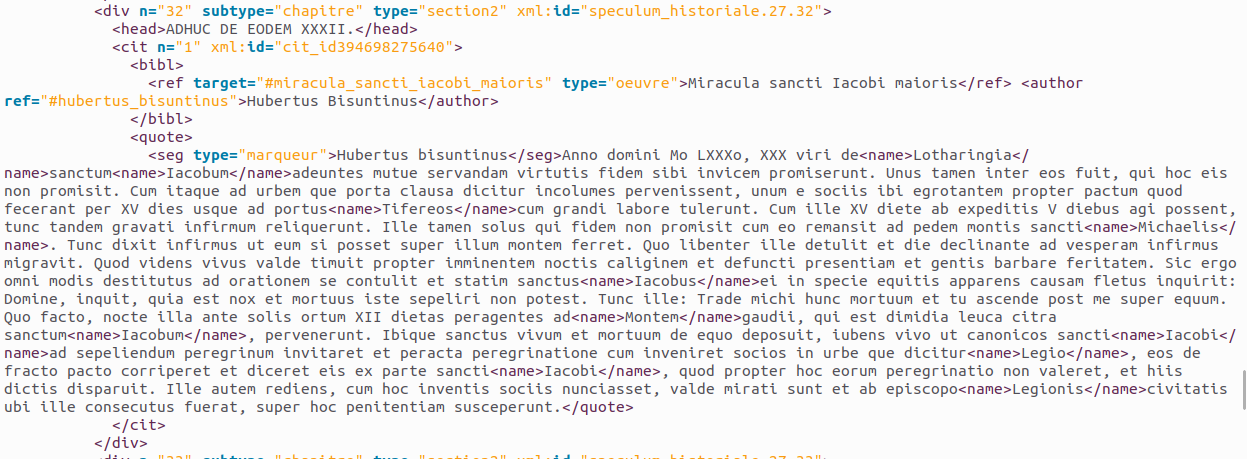
\includegraphics[width=0.8\linewidth]{images/problemnumero2.png}}
	\caption{Texte de l'encyclopédie qui est repris}
\end{figure}

Le dernier problème a résidé dans la division des \index{Encyclopédies}encyclopédies en citations. Les liens peuvent uniquement être créés pour des citations spécifiques, alors que les numéros de chapitres indexés dans ThEMA ne fournissent que le numéro de chapitre, tandis qu'il peut y avoir plusieurs citations pour un même chapitre. Après discussion avec \index{Emmanuelle Kuhry}Emmanuelle Kuhry et \index{Isabelle Draelants}Emmanuelle Kuhry, il a été décidé de placer les liens dans la première citation de chaque chapitre. Cette approche laisse à l'utilisateur le soin de trouver le passage exact. Cette solution a été retenue en raison de la complexité et du volume de vérifications manuelles nécessaires, étant donné que parfois un passage peut être mentionné dans toutes les citations d'un chapitre ou seulement dans une seule.
	
\chapter{L'interconnexion des bases de données comme moteur de l'Open Data dans les sciences}	
Il est désormais important de remettre en perspective le travail de mise en relation réalisé ici. Ce travail s’inscrit dans une dynamique plus large d’ouverture des données de la recherche (\index{Open Data}Open Data), en contribuant à la fois à la collaboration scientifique, à la valorisation des données, et à la facilitation de leur accès pour les utilisateurs\footcite{wesselsOpenDataKnowledge2017}.


\section{Renforcement des collaborations scientifiques}
La connexion entre les deux bases de données a non seulement permis de relier des données éloignées, mais aussi de rapprocher des équipes de recherche géographiquement et institutionnellement distinctes\footnote{Je me permets de renvoyer à l'introduction pour plus de détails}.

Un rapprochement s’est opéré, notamment au niveau institutionnel. Au cours de ce stage, des réunions ont parfois été nécessaires entre les équipes des deux bases. Ces réunions avaient pour objectif non seulement de présenter l’avancement de mon travail, mais aussi de réfléchir collectivement aux défis rencontrés. Par exemple, une réunion avec \index{Marie-Anne Polo de Beaulieu}Marie-Anne Polo de Beaulieu, Elisa Lonati et \index{Isabelle Draelants}Isabelle Draelants a permis de tenir l’équipe de ThEMA informée de mes progrès alors que je collaborais avec l’équipe de SourcEncyMe. Ce moment a été crucial pour déterminer comment intégrer les \index{Récits exemplaires}récits exemplaires trouvés dans les encyclopédies au sein de ThEMA. Par ailleurs, chaque équipe a eu l’occasion de présenter son travail à l'autre avant le début du stage.

Ce rapprochement s’est également opéré au niveau des données, car j’ai réussi à connecter les deux bases qui, auparavant, étaient indépendantes. Cela a permis d’éviter la duplication des efforts et de favoriser la réutilisation des données, tout en évitant que SourcEncyMe ne devienne une base spécialisée dans les exempla, et vice versa.


\section{Valorisation des bases de données}
La mise en relation des deux bases de données a également permis de valoriser chacune d’elles.

Ce stage m’a permis d’ajouter de la valeur à ces deux bases. Pour SourcEncyMe, j’ai contribué à l’identification des \index{Récits exemplaires}récits exemplaires dans les encyclopédies, qui n’avaient pas été repérés auparavant. Ce processus pourra d’ailleurs se poursuivre grâce au code \index{XSL}XSL que j’ai développé. Pour ThEMA, j’ai enrichi la base avec de nouveaux \textit{exempla} issus des encyclopédies, notamment en traitant intégralement deux œuvres : le \index{Speculum historiale}\textit{Speculum historiale} de Vincent de Beauvais et la \textit{Summa de exemplis ac similitudinibus rerum} de Giovanni da San Gimignano. Il reste toutefois à télécharger les fichiers \index{XML}XML modifiés dans les deux bases pour rendre visible l’ensemble du travail réalisé durant mon stage\footnote{Les fichiers ont été envoyés aux deux équipes, mais restent disponibles sur mon GitHub. \url{https://github.com/Laitauchocolat34/memoire-tnah}}. Par ailleurs, les codes en annexes permettront de traiter toutes les autres encyclopédies de SourcEncyMe que je n'ai pas eu le temps de traiter pendant mon stage.

Ce stage a également contribué à rendre les deux bases de données plus accessibles et plus visibles. Les liens ajoutés augmentent la probabilité que les utilisateurs découvrent l’une des bases. J’ai aussi présenté, avec \index{Marie-Anne Polo de Beaulieu}Marie-Anne Polo de Beaulieu, le travail en cours sur les deux bases de données au collectif « Sources et données de la recherche » du \index{CRH}CRH, et un billet est prévu sur le blog de l’atelier de \index{Vincent de Beauvais}Vincent de Beauvais pour mettre en lumière ce travail. Par ailleurs, il est également envisagé d'informer le LabEx HaStec des avancées du travail.


\section{Amélioration de l'expérience utilisateur}
Enfin, la mise en relation des deux bases de données a facilité la recherche pour les utilisateurs. Auparavant, s’ils trouvaient un texte encyclopédique dans ThEMA ou un \textit{exemplum} dans SourcEncyMe, ils ne savaient peut-être pas où chercher pour obtenir plus d’informations. Désormais, un utilisateur de SourcEncyMe qui trouve un \textit{exemplum} peut consulter la bibliographie associée, découvrir d’autres \index{Récits exemplaires}récits exemplaires sur les mêmes thèmes, ou encore accéder à des textes similaires. De son côté, l’utilisateur de ThEMA pourra plus facilement retrouver le texte intégral de l’encyclopédie et identifier la source de l’auteur de l'encyclopédie. 

Cependant, pour l’utilisateur, il s’agit souvent d’un « gain marginal » dans ce type de bases de données. En général, l’utilisateur explore une base pour une raison précise et ne cherche pas nécessairement à exploiter toutes les possibilités offertes. Globalement, l’accessibilité en ligne de la base de données reste l’aspect le plus crucial, tandis que le reste peut être perçu comme un complément. Pour un utilisateur, la création et la mise en ligne d'une base de données sont plus importantes que l'établissement de liens entre différentes bases.

\chapter{De nouvelles perspectives grâce à l'interconnexion}
Il est désormais important de voir quelles perspectives offrent la connexion des deux bases données. Ce chapitre explore d'abord les avantages de cette interconnexion pour la recherche, puis présente les méthodes de visualisation qui permettent de clarifier ces connexions.


\section{Bénéfices pour la recherche de la mise en relation des deux bases de données}
La mise en relation des bases de données offre des avantages pour la recherche scientifique.

Pour le projet ThEMA, établir ce lien permettra d'approfondir l'étude déjà bien avancée des sources des \index{Récits exemplaires}récits exemplaires\footnote{Il n'existe pas d'ouvrages offrant une synthèse des sources des récits exemplaires. Les sources diffèrent d'un recueil à l'autre, ce qui rend une telle synthèse irréalisable. Cependant, certaines éditions de sources ainsi que des articles ou chapitres de revues les analysent. La base bibliographique Bibliex, consacrée aux récits exemplaires, mentionne 36 fois le mot « source ». Le liens vers Bibliex : \url{https://www.zotero.org/groups/2304628/bibliex}}. Plus précisément, cela permettra de se concentrer sur les sources encyclopédiques, qui ont jusqu'à présent été peu analysées\footnote{Il n'y a que 6 références aux encyclopédies dans Bibliex}. En examinant ces sources, nous pourrons identifier les thèmes, les sujets, ainsi que les personnages historiques ou bibliques les plus souvent repris de manière globale dans les \textit{exempla} depuis les encyclopédies. Les études des références encyclopédiques dans les recueils de récits exemplaires pourraient dépasser celles déjà réalisées par Marie-Anne Polo de Beaulieu et Jacques Berlioz sur la \textit{Scala Coeli} et le \textit{Tractatus de diversis materiis praedicabilibus}\footcite{berliozRecueilsExemplaDiffusion1994}. Nous pourrons aussi évaluer dans quelle mesure les \index{Récits exemplaires}récits exemplaires d'origine encyclopédique ont été réutilisés par les compilateurs d'\textit{exempla} ultérieurs. Les chercheurs auront l'occasion de comparer la façon dont divers auteurs ou œuvres utilisent les mêmes sources encyclopédiques dans leurs \textit{exempla}, mettant en lumière des variations stylistiques, théologiques ou culturelles. En outre, cette recherche pourrait conduire à la découverte de nouveaux \index{Récits exemplaires}récits exemplaires, étant donné que les \index{Encyclopédies}encyclopédies sont riches en textes inexplorés.

Côté SourcEncyMe, la mise en relation des deux bases pourrait éclairer les raisons pour lesquelles un auteur encyclopédique utilise un \textit{exemplum}\footnote{Il n'existe pas d'étude spécifique sur l'utilisation des récits exemplaires dans les encyclopédies, bien que le lien entre encyclopédies et \textit{exempla} ait déjà été établi, comme je l'ai mentionné dans l'introduction. La bibliographie sur les encyclopédies médiévales réalisée par Isabelle Draelants ne comporte que quelques rares mentions de récits exemplaires. Pour accéder à cette bibliographie, consultez : \url{https://ateliervdb.hypotheses.org/bibliographie-sur-lencyclopedisme-medieval}}. Cela permettra de comprendre pourquoi un auteur intègre un récit habituellement utilisé comme \textit{exemplum} dans son \index{Encyclopédies}encyclopédie, même si celui-ci ne sert pas nécessairement d'exemple. Cette démarche pourrait aussi révéler si des \index{Récits exemplaires}récits exemplaires issus de recueils d'\textit{exempla} sont repris dans des encyclopédies et pour quelles raisons. Elle offrira la possibilité d'analyser plus en profondeur la place des \index{Récits exemplaires}récits exemplaires dans les œuvres encyclopédiques, ainsi que les raisons pour lesquelles ils sont insérés dans certaines sections d'une œuvre et non dans d'autres. 


\section{Techniques de visualisation pour les relations entre \index{Récits exemplaires}récits exemplaires et \index{Encyclopédies}encyclopédies}
Pour continuer la mise en relation des bases de données, plusieurs possibilités de visualisation des données pourraient être envisagées. Elles permettraient aux chercheurs et aux utilisateurs de mieux saisir visuellement les liens entre les encyclopédies et les récits exemplaires. Une pratique de plus en plus en plus utilisée par les chercheurs dans leurs publications\footcite{jiangLiteratureReviewDevelopment2023}. \\

\begin{figure}[H]
	\centering
	\fbox{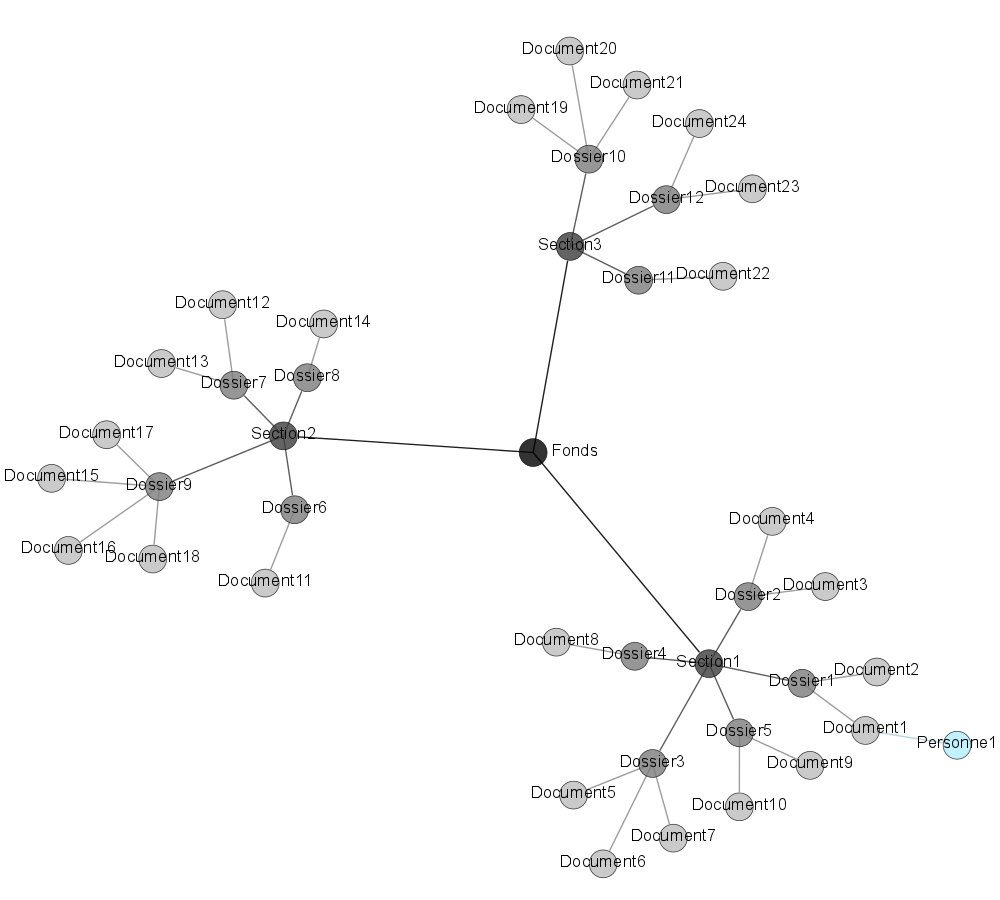
\includegraphics[width=0.2\linewidth]{images/ArchivesExemplePersonne.png}}
	\caption{Exemple de visualisation d'analyse de réseaux}
\end{figure}

Une approche intéressante serait la création de cartographies des liens établis par le travail de mise en relation des deux bases de données comme une sorte d'analyse de réseaux\footcite{beauguitteAnalyseReseauxSciences2016}. Par exemple, si plusieurs recueils d'\textit{exempla} reprennent un même morceau d'encyclopédie ils seront connectés avec des traits vers un unique point matérialisant le texte de l'\index{Encyclopédies}encyclopédie. Ces visualisations de réseaux pourraient permettre de représenter et de mieux saisir les emprunts et les influences entre les deux types de documents. 

Une autre approche intéressante serait celle du graphe de citation c'est à dire une représentation visuelle des relations de citation entre différents éléments, dans ce cas, entre les récits exemplaires au sein des \index{Encyclopédies}encyclopédies et les chapitres des encyclopédies. Le graphe de citations permet de voir rapidement quels \index{Récits exemplaires}récits exemplaires sont cités dans quels chapitres des \index{Encyclopédies}encyclopédies. Chaque lien entre un récit exemplaire et un chapitre montre une relation de citation, c'est-à-dire que le chapitre utilise ou mentionne ce récit. Si un récit exemplaire apparaît dans plusieurs chapitres, il sera connecté à chacun d'eux par des liens distincts. Cela montre non seulement où le récit est utilisé, mais aussi l'étendue de son influence à travers \index{Encyclopédies}l'encyclopédie.

Pour mettre en œuvre ces visualisations, il serait nécessaire d'adapter les fichiers XML selon les TEI Guidelines pour intégrer les métadonnées et annotations nécessaires\footcite{20GraphsNetworks}. Il faudrait ensuite avoir des logiciels comme Gephi\footcite{GephiOpenGraph} ou Cytoscape\footcite{CytoscapeOpenSource} pour développer les représentations. Pour ce qui est de l'analyse de réseaux il faudrait peut être un middleware car les deux bases de données restent séparées. Un middleware est un logiciel qui agit comme une passerelle entre des applications, outils et bases de données. 
	
	\chapter*{Conclusion}
En conclusion, j'ai réussi à relier deux bases de données \index{XML-TEI}XML-TEI en adoptant une approche techniquement réalisable, rapide, tout en maintenant une distinction institutionnelle claire. Pour ce faire, j'ai inséré semi-automatiquement des liens dans les fichiers \index{XML}XML des deux bases de données.

Cela a nécessité au préalable une étude approfondie des deux bases de données. J'ai dû m'assurer de la qualité et de la pérennité des données afin que les liens restent accessibles et durables dans le temps. J'ai opté pour la création de liens sur les données textuelles, en raison de leur utilité pour l'utilisateur et le chercheur mais aussi en raison du temps imparti. J'ai également vérifié où placer ces liens dans les \index{XML}XML et où trouver les informations nécessaires à leur création.

Ensuite, j'ai identifié précisément les textes à connecter. Cela a impliqué de rendre visibles les \textit{exempla} dans SourcEncyMe et de permettre la recherche des sources et des textes apparentés dans ThEMA. J'ai exploré la possibilité d'utiliser l'intelligence artificielle pour comparer les textes, mais j'ai finalement choisi un repérage par mots-clés dans SourcEncyMe, car les références encyclopédiques étaient déjà mentionnées dans ThEMA.

La phase suivante a été la création des liens eux-mêmes. Pour cela, j'ai indexé automatiquement les \textit{exempla} identifiés dans SourcEncyMe au sein de ThEMA. J'ai développé un code pour ajouter les liens dans ThEMA et SourcEncyMe pour les \textit{exempla} associés à des encyclopédies. Ce code permettait également de récupérer les mentions d'encyclopédies présentes dans les \textit{exempla} déjà indexés et de créer un lien chaque fois qu'une de ces encyclopédies était mentionnée dans SourcEncyMe.

Enfin, j'ai pris du recul sur le travail accompli pour démontrer qu'il contribue à un objectif plus large de la recherche, à savoir celui de l'\index{Open Data}Open Data. Ce projet a favorisé une plus grande collaboration scientifique et institutionnelle, valorisé les données, facilité l'accès des utilisateurs à ces informations, et ouvert de nouvelles perspectives pour la recherche sur les \textit{exempla} et les encyclopédies.

\

Dans le contexte de l'Open Data et de l'interopérabilité, il est crucial de réfléchir aux liens vers d'autres bases de données dès leur création. Cela simplifie grandement le processus et réduit les problématiques liées à l'adaptation à différentes structures de bases de données.

Il ne faut pas pour autant abandonner les anciennes bases de données, même si elles semblent dépassées ou moins adaptées. Des personnes y ont investi du temps et des efforts, de l'argent et il est important de ne pas laisser ce travail se perdre, mais plutôt de les faire évoluer, comme l'a permis mon stage.


	\addcontentsline{toc}{chapter}{Conclusion}
\newpage{\pagestyle{empty}\cleardoublepage}


%%%%%%%%%%%%%%%%%%

\appendix %Des appendices: tables figures, etc

\chapter[Installation de ThEMA]{Installation de ThEMA}
\textbf{Étape 1 : Chargement de la base dans eXist-db}

\begin{flushleft}
- Lancer eXist-db et ouvrir le localhost \\
- Se rendre dans l'onglet « Package Manager » \\
- Faire glisser le fichier « .xar » dans la « DROPZONE » \\
- Pour supprimer l'application ThEMA il suffit de cliquer sur l'icône poubelle dans la liste des packages installés \\ 
\end{flushleft}

\begin{figure}[H]
	\centering
	\fbox{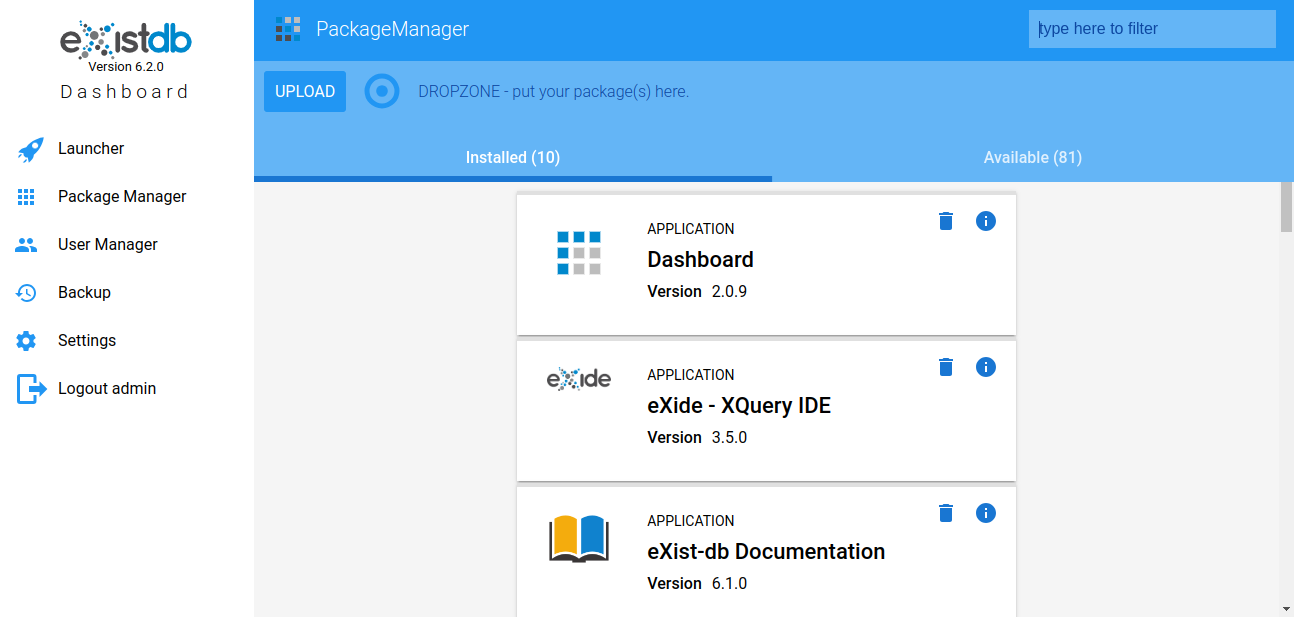
\includegraphics[width=0.8\linewidth]{images/existdbpackagemanager.png}}
	\caption{Page « Package Manager » de eXist-db}
\end{figure}

\textbf{Étape 2 : Création des groupes de sécurité} 

\begin{flushleft}
	- Faire clic droit sur l'icône eXist-db \\
	- Cliquer sur Open Java Admin Client \\ 
	- Créer un nom d'utilisateur, un mot de passe et mettre dans les favoris « localhost » \\
	- Ouvrir « Outils » puis « Éditer les utilisateurs » \\
	- Créer quatre groupes « indexer », « editor », « project-contributor » et « project-engineer » \\
	- Par défaut, eXist-db nous identifiera comme admin \\
\end{flushleft}	

\begin{figure}[H]
	\centering
	\fbox{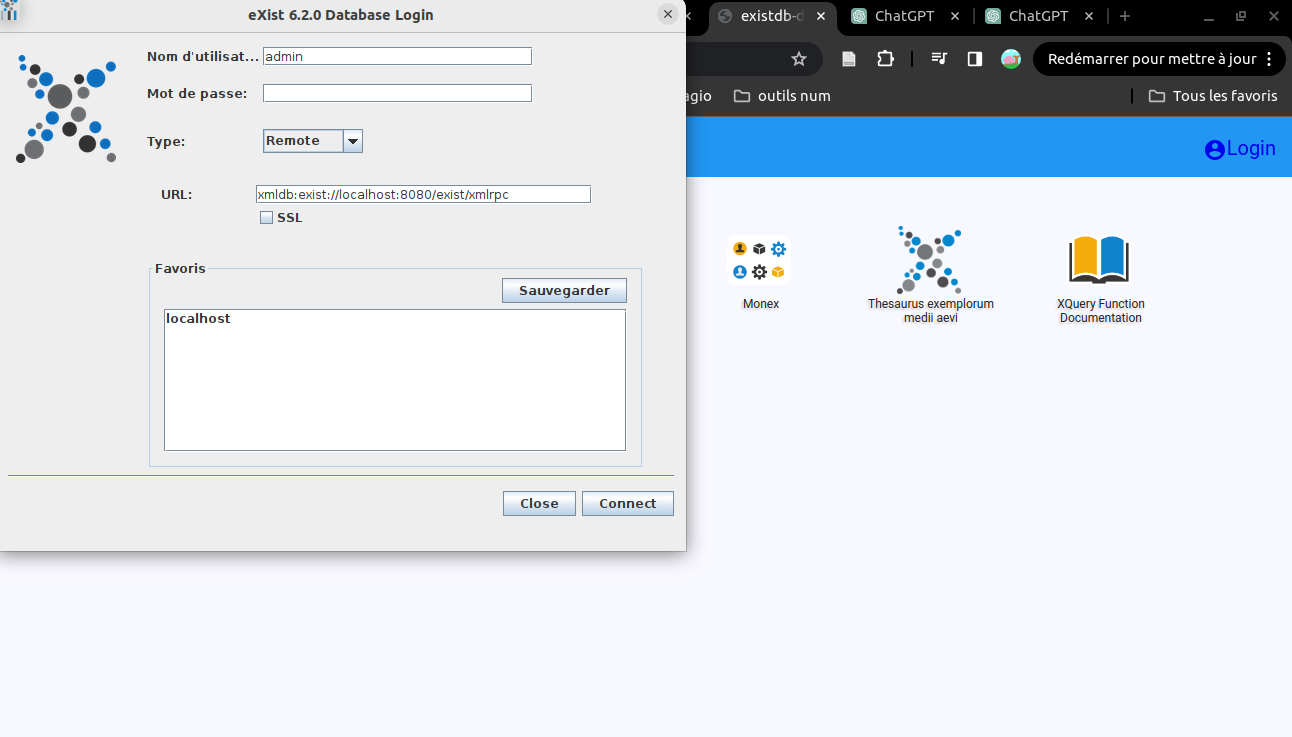
\includegraphics[width=0.6\linewidth]{images/adminexist.png}}
	\caption{Modification dans l'Admin client n°1}
\end{figure}
	
\begin{flushleft}	
	- Aller dans « apps », « thema », « modules » \\
	- Ouvrir « dbfunction » en cliquant sur « Editer les propriétaires » \\
	- Cocher « SetUID » et « SetGID » \\ 
	- Ouvrir « user.xql », cocher toutes les cases de la colonne « Execute » et passer du groub « dba » à « thema » \\

\end{flushleft}	
	
\begin{figure}[H]
	\centering
	\fbox{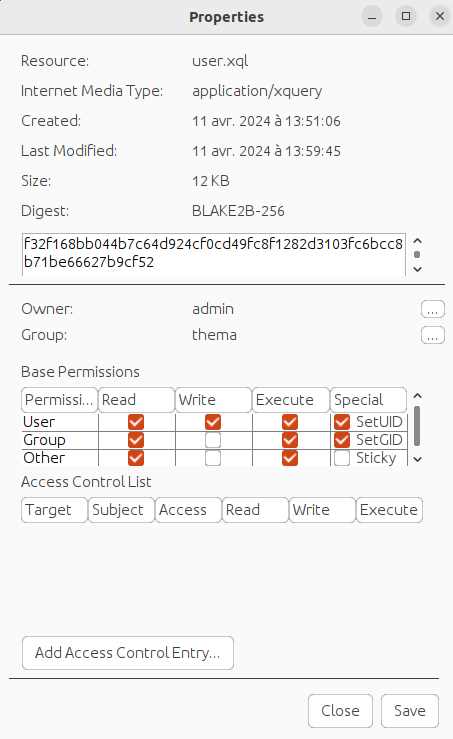
\includegraphics[width=0.3\linewidth]{images/dba.png}}
	\caption{Modification dans l'Admin client n°2}
\end{figure}
	
\textbf{Étape 3 : Compléter la base} 

\begin{flushleft}	
	- Aller dans eXide \\ 
	- Aller dans « File » puis « Manage » \\
	- Se rendre à l'endroit de l'arborescence et cliquer sur « Upload Files » \\ 
	- Faire glisser les données et appuyer sur « done » quand le chargement est terminé \\
	- Les dossiers et fichiers à ajouter sont ceux présents dans la copie de la base mais qui ne sont pas dans eXist-db \\
	- Ne pas mettre trop de fichiers en même temps et bien attendre que la roue dentée arrête de tourner \\
	- vérifier que les documents sont bien implémentés \\
	
	 - Se rendre dans « apps », « thema » \\
	 - Lancer les fichiers « .xconf » en appuyant sur « Eval » \\
	 - En cas d'ajouts de données, il sera nécessaire de lancer à nouveau l'évaluation \\ 
	 - Modifier « var base URL = » avec : « 'https://localhost:8080/exist/apps/thema/' » \\
\end{flushleft}
	
\begin{figure}[H]
	\centering
	\fbox{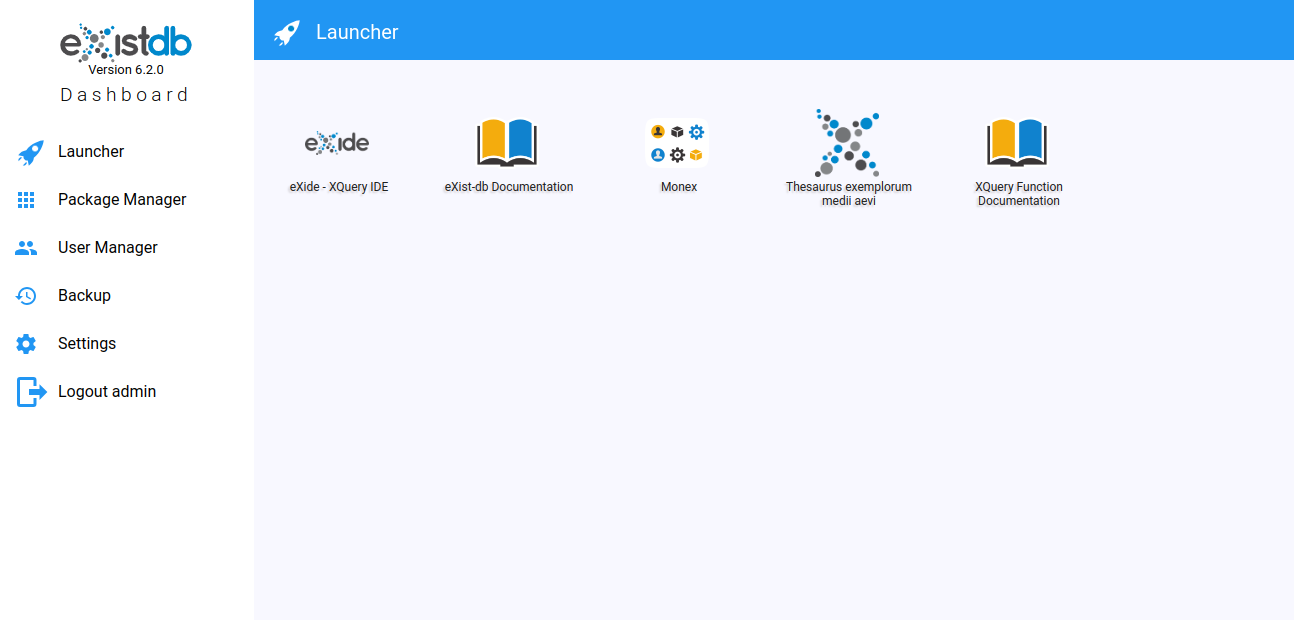
\includegraphics[width=0.8\linewidth]{images/exideexistdb.png}}
	\caption{Page d'accueil d'eXist-db}
\end{figure}

\begin{figure}[H]
	\centering
	\fbox{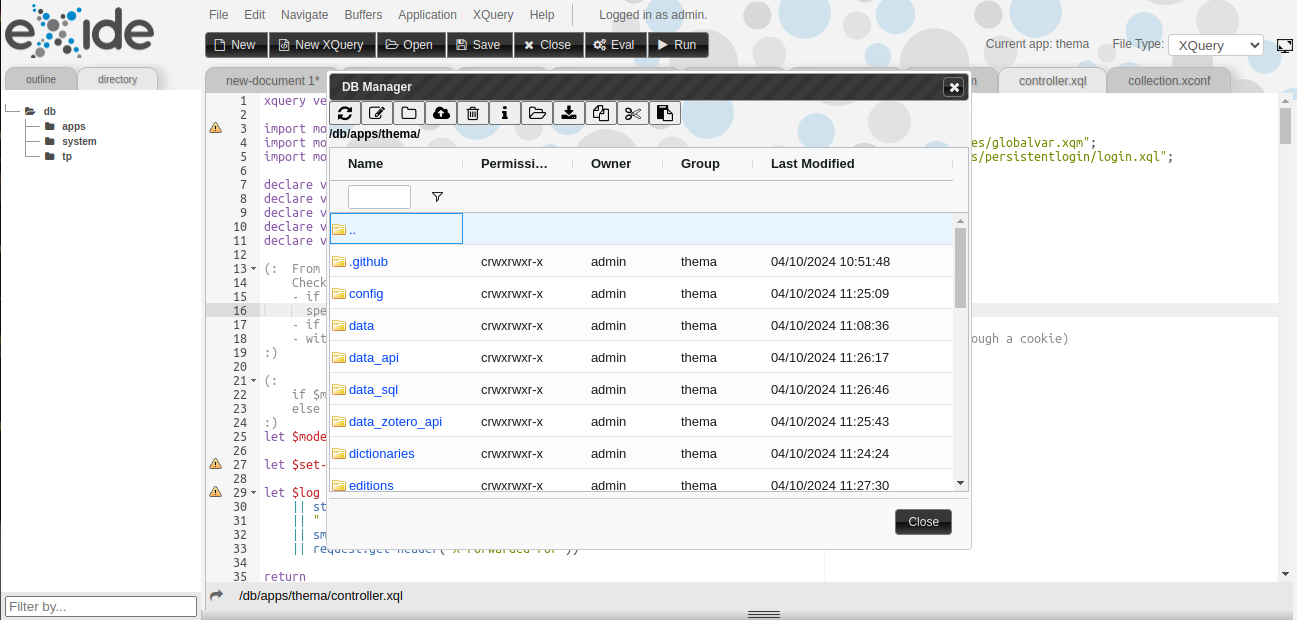
\includegraphics[width=0.8\linewidth]{images/implementationexide.png}}
	\caption{Page d'accueil « Upload Files »}
\end{figure}
	
\textbf{Étape 4 : Lancer et éteindre la base de données} 
	
\begin{flushleft}
	- Se rendre dans le « Launcher » de eXist-db \\
	- Cliquer sur « ThEMA » \\
	- Essayer toutes les fonctionnalités pour vérifier s'il n'y a pas de bogue \\
	
	- Cliquer sur l'icône eXist-db et cliquer sur « Stop server » \\
	- Cliquer sur « Quit »\\
	- Si cette manipulation n'est pas réalisée, il y a un risque d'altération des données et de la structure de la base \\
	
\end{flushleft}
	
\textbf{Étape 5 : Création d'un back-up} 
	 
\begin{flushleft}
	 - Chercher l'endroit où est installé eXist-db sur l'ordinateur \\
	 - Ouvrir le fichier « conf.xml » et remplacer « true » par « false » dans « posix-chown-restricted » \\
	 - Ajouter dans les balises « <scheduler> </scheduler> », le code suivant : \\
	 
\end{flushleft}

\begin{lstlisting}[breaklines=true]
	 	<job type="system" class="org.exist.storage.ConsistencyCheckTask"  cron-trigger="0 10 2 * * ?">
	 	<parameter name="output-dir" value="backup"/>
	 	<parameter name="zip" value="yes"/>
	 	<parameter name="backup" value="yes"/>
	 	<parameter name="incremental" value="no"/>
	 	<parameter name="incremental-check" value="no"/>
	 	</job>
\end{lstlisting}

\begin{flushleft}
	 - Aller dans « Fenêtre », « Afficher la vue », « Explorateur de sources de données » \\
	 - Se connecter à eXist-db localhost \\
\end{flushleft}

\begin{figure}[H]
	\centering
	\fbox{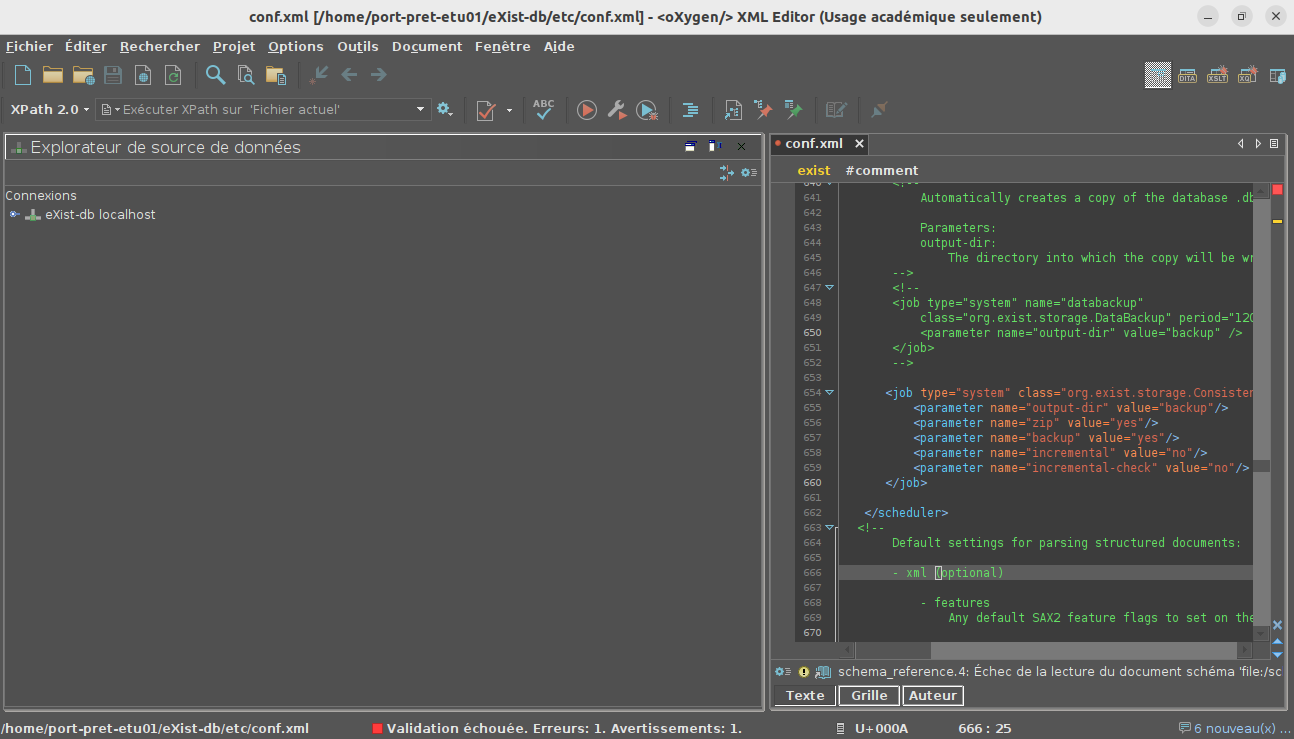
\includegraphics[width=0.8\linewidth]{images/oxygen.png}}
	\caption{Utilisation de Oxygen pour coder en lien avec eXist-db}
\end{figure}
\pagestyle{empty}

\chapter[Fonctionnement de ThEMA]{Fonctionnement de ThEMA}

	\section{La structure de ThEMA}
\textbf{Dossier 1 : Data} 
\begin{flushleft}
	- Les dossiers « TC » représentent les différents recueils d'\textit{exempla} \\ 
	- Les fichiers « TC » représentent l'écran d'accueil du recueil \\
	- Les fichiers « TE » sont les différents \textit{exempla} indexés \\
	- Les fichiers sont listés par ordre d'ajout sur la base \\
	- Liste des mots clefs \\
	- Liste des manuscrits \\
	- Liste de la bibliographie \\
	- Liste des groupes de mots-clefs \\
	- Liste des lieux \\
	- Liste des personnes \\
	- Liste des langues \\
	- Liste des contextes \\
	- Un fichier « xconf » sert à indexer les données dans la base une fois ajoutées \\
\end{flushleft}

\textbf{Dossier 2 : data\_zotero\_api} 
\begin{flushleft}
- Ce dossier contient l'\index{API} de zotero.
\end{flushleft}
	
\textbf{Dossier  3 : editions} 
\begin{flushleft}	
	- Contient les éditions électroniques au format \index{XML} de quelques recueils d'\textit{exempla} \\
	- Contient aussi un fichier « .xconf » pour leur indexation dans la base \\
\end{flushleft}	
	
\textbf{Dossier  4 : editorial} 
\begin{flushleft}	
	- Contient les informations éditoriales du projet ThEMA en 5 langues \\
	- Contient un fichier avec les remerciement en 5 langues \\
\end{flushleft}		
	
\textbf{Dossier 5 : modules}
\begin{flushleft}	
	- Contient un dossier contenant le code pour générer des PDF 
	- Contient tous les fichiers faisant tourner la base de données.
	- Contient deux types de fichiers : xqm et xql
\end{flushleft}	

\textbf{Dossier 6 : pdf} 
\begin{flushleft}	
	- Contient les présentations des recueils au format PDF.
\end{flushleft}	
	
\textbf{Dossier 7 : ressources}
\begin{flushleft}		
	 - Contient un dossier « css » pour l'aspect visuel de l'application \\
	 - Contient un dossier « fontawesome » pour la police fontawesome \\
	 - Contient un dossier « fonts » pour les autres polices de caractères \\
	 - Contient un dossier « graphics » avec toutes les icônes \\
	 - Contient un dossier « images » pour les images de manuscrits présent dans la base \\
	 - Contient un dossier « js » pour le code en JavaScript \\
	 - Contient un dossier « json » pour le code json \\
\end{flushleft}	
 
\textbf{Dossier 9 : temp}
\begin{flushleft}	
	 - Dossier vide
\end{flushleft}	
	
	\section{Le fonctionnement de ThEMA}
	Quand une requête arrive d'internet ou du localhost vers eXist-db, elle passe par Getty. Il s'agit d'une interface facilitant le dialogue entre internet et eXist-db. Pour coder ThEMA, il n'est pas nécessaire de consulter le code de Getty.
	
	Le premier fichier important est controller.xql. C'est ici que la requête arrive après être passée par Getty. Il s'agit d'un échangeur qui va guider les requêtes vers différents endroits de la base de données. Il ne faut pas modifier ce code, sinon l'application ne fonctionnera plus.
	
	Ensuite, la majorité du code se trouve dans le dossier modules. Le premier élément important dans ce dossier est le fichier globalvar.xqm. Ce code est un module \index{XQuery} qui définit plusieurs variables globales pour stocker des chemins d'accès, des URL et d'autres informations utiles. Globalement, il permet de créer des raccourcis.
	
	L'autre module important est page.xqm. Il s'agit d'un module principal affichant la page d'accueil de la base dans un navigateur internet. C'est à partir de ce module qu'il est possible de naviguer sur le site de ThEMA. Les autres pages sont appelées avec « import module namespace ».
	
	Le reste du site fonctionne comme « page.xqm ». En haut se trouvent les appels à d'autres pages, et en bas le code que le fichier traite. Il faut remonter progressivement les pages pour accéder aux données.
	
	Pour commenter le code, il faut utiliser « <!-- --> » pour du XML, « (: :) » pour du XQuery et « /* */ » pour du JavaScript.
	
	Dans le site, le visuel est géré par les fichiers JS, tandis que les données et le HTML sont gérés par \index{XQuery}.
	
	\section{La façon de créer un recueil et indexer des \textit{exempla}}
	
\textbf{Créer un recueil}
\begin{flushleft}	
	- Se rendre dans « Liste des recueils » \\
	- Cliquer sur « Créer un recueil » \\
	- Écrire le nom du recueil de préférence en langue originelle \\
	- Choisir l'édition scientifique sur laquelle se base l'indexation \\
	- Choisir les utilisateurs pouvant indexer les \textit{exempla} du recueil \\
\end{flushleft}	
	
	\begin{figure}[H]
		\centering
		\fbox{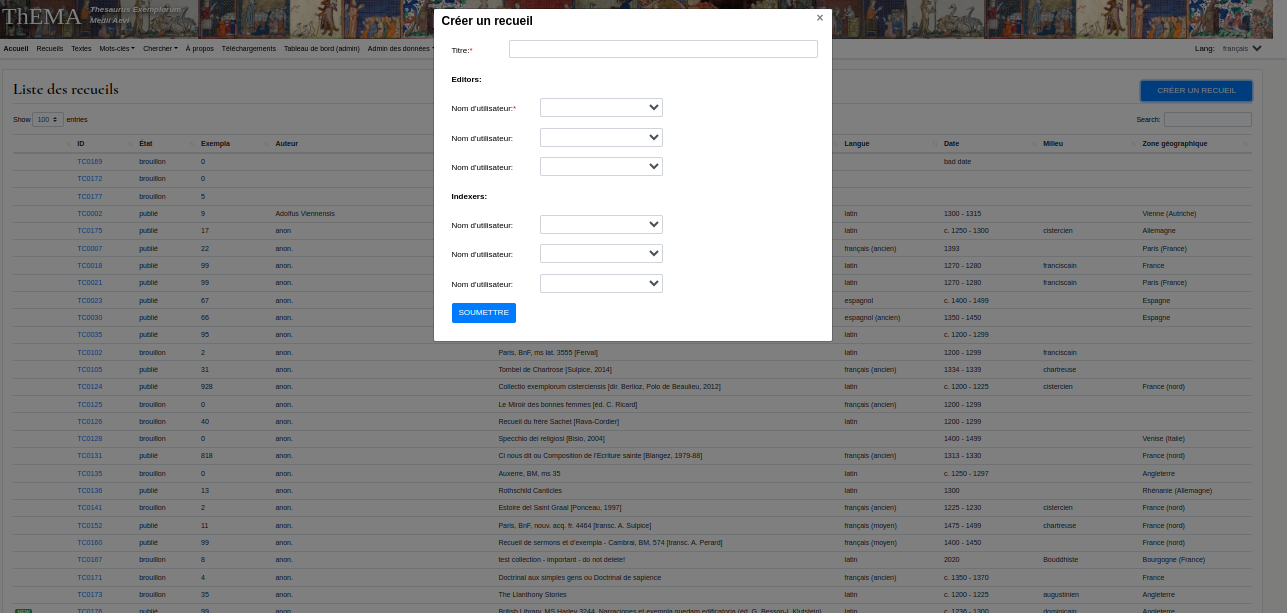
\includegraphics[width=0.6\linewidth]{images/creerrecueil.png}}
		\caption{Créer un recueil}
	\end{figure}

\textbf{Modifier un recueil}
\begin{flushleft}	
	- Se rendre dans la liste des recueils et en sélectionner un \\
	- Cliquer sur « Modifier » \\
	- Attendre la fin du chargement \\
	- Remplir les champs \\
	- Si les volets déroulant ne contiennent pas les informations nécessaires il faut se rendre dans « Admin des données » et les ajouter \\
\end{flushleft}	

	\begin{figure}[H]
	\centering
	\fbox{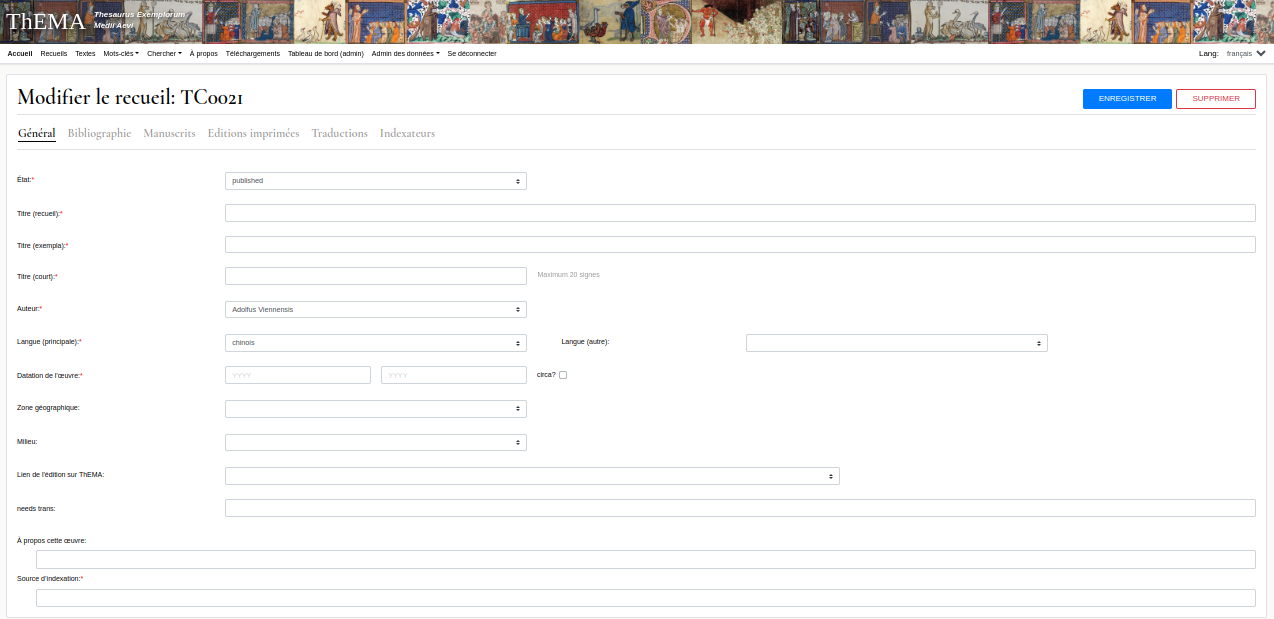
\includegraphics[width=0.6\linewidth]{images/creerrecueill.png}}
	\caption{Modifier un recueil}
	\end{figure}
	
\textbf{Créer ou modifier un \textit{exemplum}}
\begin{flushleft}	
	- Se rendre dans le tableau de bord ou dans le recueil créé \\
	- Cliquer sur « Créer un \textit{exemplum} \\
	- Attendre la fin du chargement \\
	- Compléter les champs \\
	- Si les volets déroulant ne contiennent pas les informations nécessaires il faut se rendre dans « Admin des données » et les ajouter \\
	- Enregistrer les modifications avec le bouton vert en haut à droite \\
	- Pour supprimer un \textit{exemplum} appuyer sur le bouton rouge « supprimer » \\
\end{flushleft}	
	
\begin{figure}[H]
	\centering
	\fbox{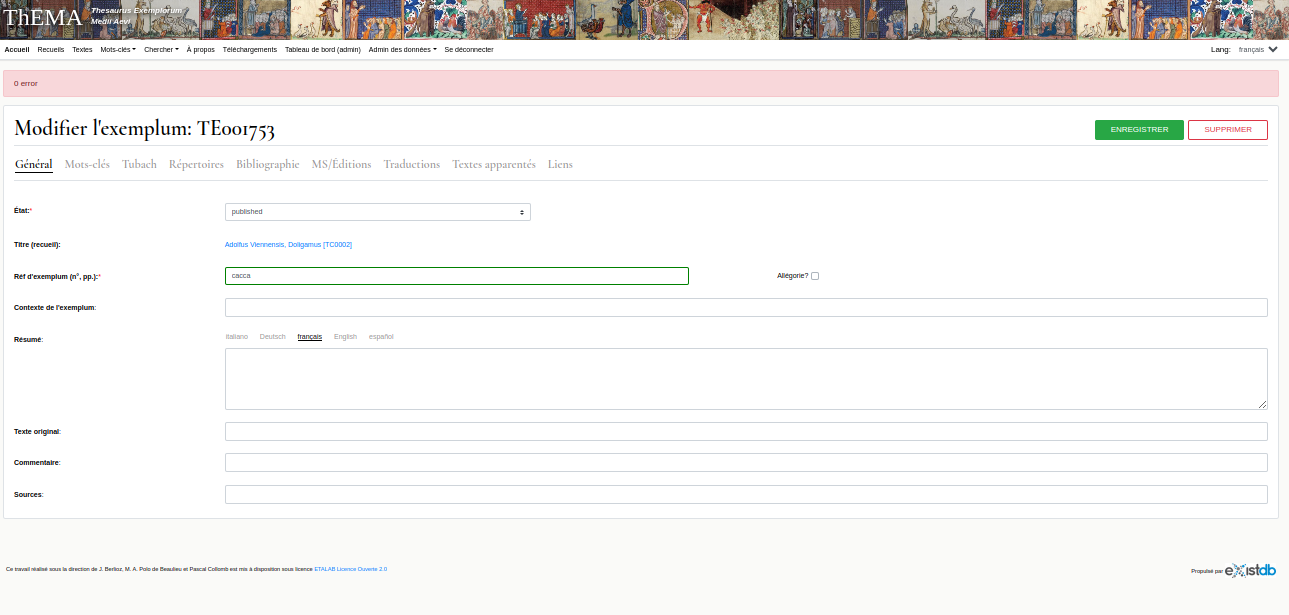
\includegraphics[width=0.6\linewidth]{images/creerexemplum.png}}
	\caption{Créer un \textit{exemplum}}
\end{figure}
\pagestyle{empty}

\chapter[Code pour classer par ordre alphabétique des récits exemplaires avec un code Python]{Code pour classer par ordre alphabétique les récits exemplaires avec un code \index{Python}Python}
\begin{lstlisting}[breaklines=true]
	from pathlib import Path
	from lxml import etree
	import re
	
	p = Path('../data')
	exempla_variable = list(p.glob('TC*/*.xml'))
	# print(exempla_variable)
	
	def roman_to_arabic(roman):
	"""takes roman numbers (param roman) and returns arabic numbers"""
	roman_numerals = {'I': 1, 'V': 5, 'X': 10, 'L': 50, 'C': 100, 'D': 500, 'M': 1000}
	arabic = 0
	prev_value = 0
	for numeral in reversed(roman):  # reversed affiche une variable dans le sens inverse.
	value = roman_numerals[numeral]
	if value < prev_value:
	arabic -= value
	else:
	arabic += value
	prev_value = value
	return arabic
	
	def lettre_en_numero(lettre):
	"""takes letter and returns its numeral position (a = 1, b = 2, etc)"""
	lettre = lettre.lower()
	if lettre.isalpha() and len(lettre) == 1:
	return ord(lettre) - ord('a') + 1 # Passe par la table unicode. A partir de "a" (97) définit le numéro des autres lettres de l'alphabet
	else:
	return -1
	
	def bis_to_two(texte):
	""" takes "bis" and return "2" """
	if texte.lower() == "bis":
	return "2"
	
	
	
	# Définir une liste de tuples contenant chaque regex et le traitement associé
	regex_patterns_and_handlers = [
	
	#### Sample : IV, 25 [82] == 82-1
	(r"^\d+[\.,\(\(] ?[\dA-Za-z]+$", lambda match: match[0].replace(' ', '').replace('.', '-').replace(',', '-')),
	
	#### Sample : 175b == 175-2
	(r"^(\d+)([A-Za-z])?$", lambda match: f"{match.group(1)}-1" if not match.group(2) else f"{match.group(1)}-{lettre_en_numero(match.group(2))}"),
	
	# 
	(r"^\s*\d+(\.)?\s*$", lambda match: match[0].replace(' ', '').replace('.','')),
	
	#### Sample : XV, 15 == 15-15
	(r"^([IVXLCDM]+) ?,?\s*(\d+(,\s*\d+)*)?\,?$", lambda match: f"{roman_to_arabic(match[1].replace(',', '-').replace(' ', ''))}-{match[2].replace(', ', '-') if match[2] else ''}"),
	
	#### Sample : [52] == 52 
	(r"\[(\d+)([A-Za-z])?\]", lambda match: f"{match.group(1)}-{lettre_en_numero(match.group(2)) if match.group(2) else '1'}"), 
	
	#### Sample : 1, 2, 3 == 1-2-3
	(r"^\d+(\.\d+)?(,\s*\d+(\.\d+)?)*$", lambda match: re.sub(r'\s*,\s*', '-', match[0])),
	
	#### The Llanthony Stories : 25 == 25. The Llanthony Stories
	(r"The Llanthony Stories : (\d+)$", lambda match: match.group(1)), 
	
	#### 720, 1-8 == 720. Ci nous dit
	(r"(\d+)([A-Za-z])?, ?\d+-\d+", lambda match: f"{match.group(1)}-{lettre_en_numero(match.group(2)) if match.group(2) else '1'}"),
	
	#### Paris, BnF lat. 16481, Sermo 12, 2' == 12-2. Paris, BnF lat 16481-16482
	(r"Paris, BnF lat\. (16481|16482), Sermo [A-Za-z]?(\d+)(?:, (\d+))?", lambda match: f"{match.group(2)}-{match.group(3) if match.group(3) else ''}"),
	
	####  Sample : F13 == 1-13. Fabulae et parabolae
	(r"^(F|P|CS|CT)(\d+)([A-Za-z])?", lambda match: f"{1 if match.group(1) == 'F' else (2 if match.group(1) == 'P' else (3 if match.group(1) == 'CS' else 4))}-{match.group(2)}-1" if match.group(3) else f"{1 if match.group(1) == 'F' else (2 if match.group(1) == 'P' else (3 if match.group(1) == 'CS' else 4))}-{match.group(2)}"),
	
	#### Sample : I, 3 Exemplum 12 (Collet) == 12. Livre du jeu d'échecs
	(r"Exemplum ?(.)? (\d+)\.? ? ?\( ?C?c?ollet\)", lambda match: match.group(2)),
	
	#### Sample : n°1 == 1 
	(r"^n° ?(\d+)$", lambda match: match.group(1)), # "n°1"
	
	# Sample : None = None 
	(r"^(None)$", lambda match: match.group(1)), # Les cas de valeurs vide "None"
	
	##### Sample : RMEx_0126b = 0126-2. Érdy Codex
	(r"RMEx_(\d+)([a-zA-Z])?", lambda match: f"{match.group(1)}-{lettre_en_numero(match.group(2))}" if match.group(2) else match.group(1)), # "RMEx_0126b
	
	#### Sample : 5 (1) == 5-1. Dits de Jehan de Saint-Quentin
	(r"^(\d+) ?\((\d+)\)\.?$", lambda match: f"{match.group(1)}-{match.group(2)}"), # 5 (1)
	
	# Sample : Le dit de la bourjosse de Romme, p. 39-46 == 4. 
	(r"^([A-Za-z])\.?\,? (L?D?)", lambda match: str(lettre_en_numero(match.group(1)))), 
	
	#### Sample : Parabole 15B = '15-2. Parabolaire
	(r"^Parabole (\d+)([A-Za-z])?$", lambda match: f"{match.group(1)}-{lettre_en_numero(match.group(2))}" if match.group(2) else match.group(1)),
	
	# Sample : exemple 49, p. 30 du texte hébreu == 49-1. Sefer Hamaassiyot
	(r"^exemple ?(\d+)([A-Za-z])?(.*)?du texte hébreu?(\))?", lambda match: f"{match.group(1)}-{lettre_en_numero(match.group(2)) if match.group(2) else '1'}"), 
	
	#### Sample : strophes 285-290 == 285. Libro de buen amor 
	(r"strophes (\d+)-(\d+)", lambda match: match.group(1)),
	
	# Sample : XVI. Exemplum de tonellis olei == 16. Disciplina clericalis
	(r"^([IVXLCDM]+)(\.)? Exemplum de", lambda match: f"{roman_to_arabic(match.group(1))}"), 
	
	# Sample : fol. 4, n° 1 = 1. British Library, Add. 27909B
	(r"^fol\. (\d+)([A-Za-z])?,?\.?-?(\d+)?([A-Za-z])?\,? n° (\d+)([A-Za-z])?", lambda match: f"{match.group(5)}-{lettre_en_numero(match.group(6)) if match.group(6) else '1'}" if match.group(6) else match.group(5)),
	
	#### Sample : OS013_E06 == 013-06. Sermones de sanctis Biga salutis intitulati
	(r"^OS(\d+)_E(\d+)$", lambda match: f"{match.group(1)}-{match.group(2)}"), 
	
	# Sample : CPS-H 8 = 2-8
	(r"^(?!CPS-H\s)(\d+)([a-zA-Z])?,\s*pp?\.?\s*(\d+)(?:-(\d+))?", lambda match: f"1-{match.group(1)}-{lettre_en_numero(match.group(2)) if match.group(2) else '1'}" if match.group(4) else f"{match.group(1)}" if not match.group(3) else f"{match.group(1)}-{match.group(3)}" if match.group(4) else f"{match.group(1)}" if not match.group(3) else f"{match.group(1)}-{lettre_en_numero(match.group(2)) if match.group(2) else ''}"), # Collectaneum
	
	# Sample : 65 [b] == 65-2
	(r"^(\d+)\s*(?:\[|\s+)([A-Za-z])\]?$", lambda match: f"{match.group(1)}-{lettre_en_numero(match.group(2))}"), # 65 [b]
	
	# Sample : Lettre 112, p. 276, l. 9 – p. 277, l. 8' == 112-276-9
	(r"^Lettre (\d+), p\. ?(\d+), l?L?\. (\d+)(?: –?-? p\. (\d+), l\. (\d+))?", lambda match: f"{match.group(1)}-{match.group(2)}-{match.group(3)}"),
	
	# Sample : Livre II, chapitre 28, col. 572 C = 2-28-572
	(r"^Livre (I{1,3}), chapitre (\d+), col\. (\d+)(?:\s+[A-Z]\s*(?:-\s*[A-Z])?)?$", lambda match: f"{roman_to_arabic(match.group(1))}-{match.group(2)}-{match.group(3)}"),
	
	# Sample : Livre I, chapitre 26, col. 537 B - 538 A == 1-26-537
	(r"^Livre (I{1,3}), chapitre (\d+), col\. (\d+) [A-Za-z] - (\d+) [A-Za-z]", lambda match: f"{roman_to_arabic(match.group(1))}-{match.group(2)}-{match.group(3)}"),
	
	# Sample : Predicazione della quaresima 1425 (Firenze S. Croce, 4 febbraio-8 aprile), XXXIX, 1. == 1425-39-1
	(r"^.* (\d{4}) \(Firenze S\. Croce\, \d+ febbraio\-\d+ aprile\), ([IVXLCDM]+), (\d+)\.$", lambda match: f"{match.group(1)}-{roman_to_arabic(match.group(2))}-{match.group(3)}"),
	
	# Predicazione della quaresima 1424 (Firenze, S. Croce, 8 marzo-3 maggio), XXIII, 2. == 1424-23-2
	(r"^.* (\d{4}) \(Firenze\, S\. Croce\, \d+ marzo\-\d+ maggio\), ([IVXLCDM]+), (\d+)\.$", lambda match: f"{match.group(1)}-{roman_to_arabic(match.group(2))}-{match.group(3)}"),
	
	# Sample : Prediche della primavera 1425 (Siena, chiesa di S. Francesco e Piazza del Campo, 20 aprile-10 giugno), VII, 6. == 1426-7-6
	(r"^.* (\d{4}) \(Siena\, chiesa di S\. Francesco e Piazza del Campo\, \d+ aprile\-\d+ giugno\), ([IVXLCDM]+), (\d+)\.$", lambda match: f"{int(match.group(1))+1}-{roman_to_arabic(match.group(2))}-{match.group(3)}"),
	
	# Sample : Bernardino da Siena, Prediche volgari sul Campo di Siena 1427 [ed. Delcorno, 1989], XXV, 5. == 1427-25-5
	(r"^.* (\d{4}) \[ed\. Delcorno\, 1989\], ([IVXLCDM]+), (\d+)\.$", lambda match: f"{match.group(1)}-{roman_to_arabic(match.group(2))}-{match.group(3)}"),
	
	# Sample : L’usurier repentant – exemplum ajouté après le chapitre II. 34 == 2-34
	(r"(distinctio)?(chapitre)?(distinction)? ([IVXLCDM]+)\.?\s?(\d+)?\.?$", lambda match: f"{roman_to_arabic(match.group(4))}-{match.group(5) if match.group(5) else '1'}"),
	
	# Sample : LES OEUVRES DE MISERICORDE, 890 == 890
	(r"LES OEUVRES DE MISERICORDE, (\d+)", lambda match: match.group(1)),
	
	# Sample : 273bis == 273-2
	(r"(\d+) ?(bis)", lambda match: f"{match.group(1)}-{bis_to_two(match.group(2))}"),
	
	# sample : Sermones De sanctis, [éd. Maggioni, en cours], 430a - 2 = 430-1-2
	(r"Sermones De sanctis\, \[éd\. Maggioni, en cours\]\, (\d+)([A-Za-z]) - (\d+)?", lambda match : f"{match.group(1)}-{lettre_en_numero(match.group(2))}-{match.group(3)}"),
	
	# Sample : Additiones: 6 == 6
	(r"Additiones: (\d+)", lambda match: match.group(1)),
	
	# Sample App., I, 1 == 1-1
	(r"App\.\, ([IVXLCDM]+)\, (\d+)", lambda match: f"{roman_to_arabic(match.group(1))}-{match.group(2)}"),
	
	# Sample CPS-H 13 == 1-13
	(r"^CPS-H (\d+)", lambda match: f"2-{match.group(1)}"),
	
	# Sample 1, 21, 4b =  1-21-4-2
	(r"^(\d+), (\d+), (\d+)([A-Za-z])", lambda match: f"{match.group(1)}-{match.group(2)}-{match.group(3)}-{lettre_en_numero(match.group(4))}"),
	
	# Opusculum de naturis animalium, c. 9 (f. 8r) == 9-8
	(r"Opusculum de naturis animalium, c\. (\d+) \(f\. (\d+)[A-Za-z]\)", lambda match: f"{match.group(1)}-{match.group(2)}"),
	
	
	
	# CORRIGER  
	(r"^p. ?(\d+)([A-Za-z])?([A-Za-z])? ?-?([A-Za-z])?-? ?([A-Za-z])?-?(\d+)?([A-Za-z])?([A-Za-z])?$", lambda match: '-'.join(filter(None, map(lambda x: str(lettre_en_numero(x)) if x and x.isalpha() else x, match.groups())))), # Les sermone "p. 52b"
	
	# Sample : Sermo 67 §19, p. 870 = 67-19-870. Sermons et visite pastorale
	(r"^Sermo (\d+) § ?(\d+), p\. (\d+(?:-\d+)*)$", lambda match: f"{match.group(1)}-{match.group(2)}-{match.group(3).replace('-', '-')}"),
	]
	
	file_namespace = {"tei":"http://www.tei-c.org/ns/1.0"}
	
	# Pour calculer le pourcentage de modificcations réalisé
	total_titles = 0 
	unmodified_titles = 0
	
	for file in exempla_variable:
	tree = etree.parse(file)
	
	title_index = tree.xpath(".//tei:teiHeader//tei:title/tei:desc[@type='title_index']", namespaces=file_namespace)
	
	if len(title_index) > 0:
	text_title = title_index[0].text
	original_text_title = text_title  # Stocker la valeur d'origine
	modified = False  # Variable de contrôle
	for regex_pattern, handler in regex_patterns_and_handlers:
	regex = re.compile(regex_pattern)        
	query = re.search(regex, str(text_title))
	if query:
	text_title = handler(query)
	print(f"++++ '{original_text_title}' ('{query[0]}' = '{text_title}')")
	modified = True  # Modification effectuée
	break  # Sortir de la boucle une fois une modification effectuée
	if not modified:  # Si aucune modification n'a été effectuée
	print(f"---- '{original_text_title}' (not modified)")
	unmodified_titles += 1
	total_titles += 1
	
	percentage_unmodified = (unmodified_titles / total_titles) * 100
	print(f"Percentage of unmodified titles: {percentage_unmodified}%")
	
	
	# title_index[0].attrib['subtype'] =  subtype_text
	# permet de print la balise
	# print(etree.tostring(title_index[0]))
	# result_tree = etree.tostring(tree, encoding='utf-8', xml_declaration=False, doctype="", pretty_print=True)
	# result_tree = result_tree.decode('utf-8')
	# print(result_tree)
	# with open(file, 'w') as writting:
	#     writting.write(result_tree)
	# print("Done")
	
\end{lstlisting}
\pagestyle{empty}

\chapter[Code pour classer par ordre alphabétique des récits exemplaires avec un code \index{XQuery}XQuery]{Code pour classer par ordre alphabétique des \index{Récits exemplaires}récits exemplaires avec un code XQuery}
\subsection{Code pour vérifier la place des \textit{exempla}}

		\begin{lstlisting}[breaklines=true]
			xquery version "3.1";
			
			declare namespace tei="http://www.tei-c.org/ns/1.0";
			
			let $output :=
			let $collection-uri := "/db/apps/thema/data"
			
			let $subcollections := xmldb:get-child-collections($collection-uri)
			
			for $rec in $subcollections
			let $rec-uri := $collection-uri || "/" || $rec
			order by $rec
			let $collection := collection($rec-uri)
			let $exempla :=
			for $exemplum in $collection/tei:TEI
			order by $exemplum/@xml:id
			return $exemplum
			for $ex at $i in $exempla
			(:   let $update :=  local:insert-number($ex/@xml:id, $i) :)
			return
			"UPDATED collection " || $rec-uri || " exempla ID " || $ex/@xml:id || " has position " || $i || " (" || $ex//tei:titleStmt/tei:title/tei:desc[@type eq "title_index"] || ")"
			
			
			return
			xmldb:store("/db/apps/thema/data-test", "number_check.txt", string-join($output,"&#10;"))
		\end{lstlisting}

\subsection{Modification des données posant un problème}
		
		\begin{lstlisting}[breaklines=true]
			xquery version "3.1";
			
			declare namespace tei="http://www.tei-c.org/ns/1.0";
			
			
			let $collection-uri := "/db/apps/thema/data"
			let $subcollections := xmldb:get-child-collections($collection-uri)
			for $rec in $subcollections
			let $rec-uri := $collection-uri || "/" || $rec
			let $collection := collection($rec-uri)
			let $exempla := $collection/tei:TEI
			let $sorted-exempla :=
			if ($rec = "TC0131") then
			for $exemplum in $exempla
			let $firstPart := fn:substring-before($exemplum, ',')
			let $number := local:convert-to-number($firstPart)
			order by $number ascending
			return $exemplum
			else if ($rec = "TC0155" or $rec = "TC0012" or $rec = "TC0013"  or $rec = "TC0016"  or $rec = "TC0105" or $rec = "TC0138" or $rec = "TC0150" or $rec = "TC0014") then
			for $exemplum in $exempla
			let $num := local:extract-number(string($exemplum//tei:titleStmt/tei:title/tei:desc[@type eq "title_index"]))
			order by $num ascending
			return $exemplum
			else if ($rec = "TC0142") then
			for $exemplum in $exempla
			let $parts := tokenize($exemplum, ',\s*')
			let $roman := $parts[1]
			let $arabic := local:roman-to-arabic($roman)
			let $subParts := subsequence($parts, 2)
			let $firstSubPart := if (count($subParts) > 0) then local:safe-convert-to-integer($subParts[1]) else ()
			let $secondSubPart := if (count($subParts) > 1) then local:safe-convert-to-integer($subParts[2]) else ()
			order by $arabic ascending, $firstSubPart ascending, $secondSubPart ascending
			return $exemplum
			else
			for $exemplum in $exempla
			order by $exemplum/@xml:id
			return $exemplum
			for $ex at $i in $sorted-exempla
			let $update :=  local:insert-number($ex/@xml:id, $i)
			return $sorted-exempla
			
			
			
			
			
			
			declare function local:insert-number($exempla-id as xs:string, $number as xs:integer ) {
				
				let $exempla := collection("/db/apps/thema/data")/tei:TEI[@xml:id eq $exempla-id]
				return
				update insert attribute { "n" } { $number } into $exempla//tei:titleStmt/tei:title/tei:desc[@type eq "title_index"]
				
			};
			
			declare function local:convert-to-number($str as xs:string) as xs:string? {
				if (not($str)) then ()
				else
				let $parts := tokenize($str, ",\s*")
				let $number := $parts[1]
				let $letter := $parts[2]
				let $letterValue := if ($letter) then xs:string(codepoints-to-string(string-to-codepoints($letter)) - 96) else ""
				return if ($letterValue) then concat($number, ",", $letterValue) else $number
			};
			
			declare function local:extract-number($str as xs:string) as xs:integer? {
				let $match := replace($str, ".*\((\d+)\)$", "$1")
				return if ($match castable as xs:integer) then xs:integer($match) else ()
			};
			
			declare function local:roman-to-arabic($roman as xs:string) as xs:integer {
				let $map := map {
					'I': 1, 'IV': 4, 'V': 5, 'IX': 9, 'X': 10, 'XL': 40, 'L': 50, 'XC': 90, 'C': 100, 'CD': 400, 'D': 500, 'CM': 900, 'M': 1000
				}
				let $chars := fn:string-to-codepoints($roman)
				let $values := for $char in $chars
				return $map(fn:codepoints-to-string($char))
				let $total := fn:fold-left($values, 0, function($acc, $current) {
					if ($acc >= $current) then $acc + $current else $current - $acc
				})
				return $total
			};
			
			declare function local:safe-convert-to-integer($str as xs:string) as xs:integer? {
				let $numericPart := replace($str, "[^\d]", "") (: Supprime tout ce qui n'est pas un chiffre :)
				return if ($numericPart castable as xs:integer) then xs:integer($numericPart) else ()
			};
		\end{lstlisting}
\pagestyle{empty}

\chapter[Fichiers XML de ThEMA et de SourcEncyMe]{Fichiers \index{XML}XML de ThEMA et de SourcEncyMe}
\subsection{Exemple de fichier \index{XML} dans ThEMA}

\begin{lstlisting}[breaklines=true]
<?xml-model href="../schema/tei_thema.rng" type="application/xml" schematypens="http://relaxng.org/ns/structure/1.0"?>
<TEI xmlns="http://www.tei-c.org/ns/1.0" xmlns:xi="http://www.w3.org/2001/XInclude" xmlns:dc="http://dublincore.org/documents/dcm -namespace/" xml:id="TE002904" corresp="TC0011"
	type="exemplum">
	<teiHeader>
		<fileDesc>
			<titleStmt>
				<title>
					<desc type="custom_title"/>
					<desc type="title_index">p. 27b</desc>
				</title>
			</titleStmt>
			<publicationStmt>
				<authority/>
				<publisher>ThEMA (http://thema.huma-num.fr)</publisher>
				<availability status="published">
					<licence corresp="copyright-cc-by-nc-sa-4.0"/>
				</availability>
				<idno type="old_sql_id">2904</idno>
			</publicationStmt>
			<sourceDesc>
				<list type="source_details">
					<item type="source_text">
						<p/>
					</item>
					<item type="sources">
						<p/>
					</item>
					<item type="exemplum_context">
						<p>Feria quarta primae hebdomadae. Sermo I.</p>
					</item>
					<item type="commentary">
						<p/>
					</item>
					<item type="allegory">y</item>
				</list>
				<listBibl>
					<bibl type="manuscripts-editions" corresp="Z-IU7WR86C" n="t. I, p. 66-67"/>
				</listBibl>
				<list type="links">
					<item type="link" corresp="http://sermones.net/thesaurus/document.php?id=jvor_210">Sermones.net</item>
				</list>
				<list type="linked_exempla"/>
			</sourceDesc>
		</fileDesc>
		<profileDesc>
			<textClass>
				<keywords>
					<term corresp="KW0039">KW0039</term>
					<term corresp="KW0048">KW0048</term>
					<term corresp="KW0155">KW0155</term>
					<term corresp="KW0319">KW0319</term>
					<term corresp="KW0435">KW0435</term>
					<term corresp="KW0439">KW0439</term>
					<term corresp="KW0458">KW0458</term>
					<term corresp="KW0465">KW0465</term>
					<term corresp="KW0756">KW0756</term>
					<term corresp="KW0889">KW0889</term>
					<term corresp="KW1118">KW1118</term>
				</keywords>
			</textClass>
		</profileDesc>
	<xenoData/>
	<revisionDesc>
			<listChange>
				<change type="modify" resp="jrehr" when-custom="2019-08-06 14:14:00">eXist-db setup</change>
				<change type="modify" resp="jrehr" when-custom="2020-11-20 20:45:55">transformation to new schema</change>
			</listChange>
		</revisionDesc>
	</teiHeader>
	<fascimile/>
		<text>
			<body>
				<p xml:lang="de"/>
				<p xml:lang="en"/>
				<p xml:lang="es"/>
				<p xml:lang="fr">L’odeur de la bonne réputation du Christ est assimilée aux odeurs du cèdre, de la myrrhe et de la vigne qui font fuir les crapauds (représentation de la luxure), les serpents (représentation de l’avarice) et les vers (représentation de l’orgueil). Les crapauds naissent souvent des organes génitaux des cadavres des hommes.</p>
				<p xml:lang="it"/>
			</body>
		</text>
	</TEI>
\end{lstlisting}

\subsection{Exemple de fichier \index{XML} dans SourcEncyMe}

\begin{lstlisting}[breaklines=true]
<TEI xmlns="http://www.tei-c.org/ns/1.0" xmlns:xxe="http://www.unicaen.fr/mrsh/pddn/xxe/1.0/" xmlns:xsi="http://www.w3.org/2001/XMLSchema-instance" xmlns:xs="http://www.w3.org/2001/XMLSchema" xmlns:xi="http://www.w3.org/2001/XInclude" xmlns:ns="http://www.tei-c.org/ns/1.0" xmlns:hfp="http://www.w3.org/2001/XMLSchema-hasFacetAndProperty" xmlns:examples="http://www.tei-c.org/ns/Examples" xmlns:dcr="http://www.isocat.org/ns/dcr" xmlns:ad="http://ns.adobe.com/AdobeInDesign/5.0/" xmlns:a="http://ns.adobe.com/AdobeInDesign/4.0/" xsi:schemaLocation="http://www.tei-c.org/ns/1.0 http://www.unicaen.fr/mrsh/pddn/schemas/ichtya.xsd" xml:id="summa_de_exemplis_ac_similitudinibus_rerum_ed_anvers_1609">
	<teiHeader>
		<fileDesc>
			<titleStmt>
				<title ref="#liber_de_exemplis_et_similitudinibus_rerum_iohannis_de_sancto_geminiano">Summa de exemplis ac similitudinibus rerum (éd. Anvers, 1609)</title>
	<author>Iohannes de Sancto Geminiano</author>
	<respStmt>
	<persName xml:id="Beatrice.Amelotti">Beatrice Amelotti</persName>
	<resp>Mise en forme de l'édition</resp>
	</respStmt>
	<respStmt>
	<persName xml:id="Emmanuelle.Kuhry">Emmanuelle Kuhry</persName>
	<resp>Transformation TEI</resp>
	</respStmt>
	</titleStmt>
	<editionStmt>
	<edition>Avertissement : Le texte du De exemplis de G. da S. Giminiano est mis provisoirement en ligne sur SourcEncyMe, car il est régulièrement modifié et corrigé par parties ; il n’a pas encore bénéficié d’une relecture complète.</edition>
	</editionStmt>
	<publicationStmt>
	<authority>François Bougard</authority>
	<publisher>IRHT</publisher>
	<pubPlace>Aubervilliers</pubPlace>
	<date>2017</date>
	</publicationStmt>
	<sourceDesc>
	<p/>
	</sourceDesc>
	</fileDesc>
	</teiHeader>
	<text>
	<body>
	<div type="oeuvre" xml:id="de_exemplis">
	<div n="1" subtype="prologue" type="section1" xml:id="de_exemplis.prologue.1">
	<head>DE EXEMPLIS ET RERUM SIMILITUDINIBUS LOCUPLETISSIMA. PROLOGUS.</head>
	<cit xml:id="cit_idp119503344">
	<quote>Omnia facito secundum exemplar quod tibi monstratum est (inquit Apostolus). In omnibus operibus artium videmus, quod eorum opifices diriguntur et regulatur duplici exemplari&#160;: Nam qui sunt in arte periti, interius habent exemplar, scilicet formam artis, secundum quam operantur&#160;: qui vero artem addiscunt nondum eruditi in ipsa, aspiciunt ad exemplar exterius per aliquem artificem factum, sicut pueri qui scribere discunt, tenent pre oculis exemplar magistri.</quote>
	</cit>
\end{lstlisting}
\pagestyle{empty}

\chapter[Code pour recherche dans les sources et les textes apparentés de ThEMA]{Code pour recherche dans les sources et les textes apparentés de ThEMA}
sCe code ne représente pas la totalité du code présent dans le fichier search.xql. Pour économiser de la place je n'ai récupéré que le code qui permet de chercher dans les textes apparentés et dans les sources des \textit{exempla}. \\


\begin{lstlisting}[breaklines=true]
	let $paramSces := 
		if (request:get-parameter("sces", ()) != "") then 
			tokenize(request:get-parameter("sces", ()), " ") 
		else ()
	


	<div class="form-group row">
		<label class="col-md-2 col-form-label col-form-label-sm" for="search-sources">{common:labels("search-sces")}:</label>
		<input type="text" class="col-md-8 form-control form-control-sm" id="search-sources" placeholder="exemplum sources search" name="sces" accept-charset="UTF-8"/>
	</div>
	
	
	
	let $sources-in-exempla := 
		if (count($paramSces) gt 0) (: Recherche seulement si $paramSces n'est pas vide :)
			then
				let $query-sources := 
					<query>
						<bool>
							{
							for $b in $paramSces 
							return <wildcard occur="must">{normalize-space(lower-case(sch:reduced-term($b)))}</wildcard>
							}
						</bool>
					</query>
				return ($ex-items//tei:sourceDesc/tei:list[@type="source_details"]/tei:item[@type="sources"]/tei:p[ft:query(.,$query-sources,$ftqueryparams)])
			else (: Pas de recherche si $paramSces est vide :)
				$ex-items	
		return 
		

		
	(<div>
		<div class="d-flex justify-content-between border-bottom align-items-center mb-3">
			<h2 class="font-cormorant-garamond">{common:labels("search-results")}
			{
			if (count($final-ex-items) gt 0)
				then concat(" ",count($final-ex-items), " exempla")
			else (),
			if (count($sources-in-exempla) gt 0)
				then concat(" ",count($sources-in-exempla), " sources")
			else ()
			}
			</h2>
			<a class="btn btn-primary" href="{$g:URLsearch}">{common:labels("new-search")}</a>
		</div>
	
	
	
	<div class="row md-12 mb-2 d-flex align-items-center justify-content-between alert {if (count($final-ex-items) = 0 or count($sources-in-exempla) = 0)
		then "alert-danger"
		else "alert-success"}">
	
	
	
	if (count($paramSces) gt 0)
		then 
			(<strong>{common:labels("sourcessources")})</strong>, concat(" = ", string-join($paramSces," "),"; "))
	else(),
	
	
	
	if (count($final-ex-items) = 0 or count($sources-in-exempla) = 0)
		then 
			(<br/>,<strong>{common:labels("search-no-results")}</strong>)
	else ()
	

	
	if ((count($final-ex-items) gt 0) or (count($sources-in-exempla) = 0))
		then 
			<a type="button" class="btn btn-primary" href="{concat($g:URLget,"?objecttype=searchresult&amp;$objectformat=csv&amp;",request:get-query-string())}" target="_blank">{common:labels("download")} (.csv)</a>
	else ()
	
	
	if (count($sources-in-exempla) gt 0)
		then
			<div class="row">
				<div class="col-sm-12">
					<table id="tableSearch_in_sources" class="table table-sm responsive dataTable no-footer dtr-inline" style="width: 100%;" data-page-length="50" role="grid" aria-describedby="myTable_info">
						<thead>
						<tr>
							<th>{common:labels("id-coll")}</th>
							<th>{common:labels("id-ex")}</th>
							<th>{common:labels("author")}</th>
							<th>{common:labels("title")}</th>
							<th>{common:labels("exempla")}</th>
							<th>{common:labels("keywords")}</th>
						</tr>
						</thead>
						<tbody>
						{
							for $sources-exempla in $sources-in-exempla
							let $fullsources := if (count($paramSces) gt 0) then $sources-exempla/ancestor::tei:TEI else $sources-exempla
							let $coll := $coll-items/id($fullsources/@corresp)
							return 
								<tr>
									<td><a href="{$g:URLcollections || $fullsources/data(@corresp)}">{$fullsources/data(@corresp)}</a></td>
									<td><a href="{$g:URLexempla || $fullsources/data(@xml:id)}">{$fullsources/data(@xml:id)}</a></td>
									<td>{$sch:PEOPLE/id($coll//tei:author/@ref)//tei:name[@type="main"]/text()}</td>
									<td>{if ($fullsources//tei:desc[@type="title_index"]/text())
										then (concat($coll//tei:title[@type="exempla"]/text(), ": ", $fullsources//tei:desc[@type="title_index"]/text()))
										else $coll//tei:title[@type="exempla"]/text()}</td>
									<td>
										{
											if (count($paramSces) gt 0)
											then transform:transform(util:expand($sources-exempla, "expand-xincludes=no"), sch:style-hit(), ())
											else ()
										}
									</td>
									<td>
										{
											for $k in keywords:keyword-link($fullsources//tei:term[@corresp!=""]/data(@corresp))
											return <li class="list-inline-item">{$k}</li>
										}
									</td>
								</tr>
						}
						</tbody>
					</table>
				</div>
			</div>
	else ()
	}
</div>)
		
\end{lstlisting}
\pagestyle{empty}

\chapter[Code pour comparer les textes de ThEMA et de SourcEncyMe]{Code pour comparer les textes de ThEMA et de SourcEncyMe}
\begin{lstlisting}[breaklines=true]
	import pandas as pd
	from tqdm import tqdm
	from sentence_transformers import SentenceTransformer, util
	
	# Load the SBERT model for French
	model = SentenceTransformer('sentence-transformers/paraphrase-multilingual-MiniLM-L12-v2')
	
	# Function to compute similarity between two embeddings
	def compute_similarity(embedding1, embedding2):
		try:
			# Compute cosine similarity
			similarity = util.pytorch_cos_sim(embedding1, embedding2).item()
			return similarity
		except Exception as e:
			print(f"An error occurred while computing similarity: {e}")
			return None
	
	# Your manually entered text
	text1 = "De même, l'amour de la charité transforme même le mal en bien. En effet, comme le dit l'Apôtre : 'Pour ceux qui aiment Dieu, tout contribue au bien.' Un exemple en est le poirier, car les poires immatures, qui sont acides, dures et grossières, et mauvaises à manger, deviennent bonnes après cuisson au feu. De la même manière, par la cuisson et la vigueur du feu de la charité, même les grandes et lourdes adversités se transforment en bien pour l'homme, du moins pour l'âme, grâce à la patience que la charité engendre. En effet, la charité est patiente, comme le dit l'Apôtre."
	
	# Try to read the Excel file
	try:
		df = pd.read_excel('french_texts_.xlsx')
	except Exception as e:
		print(f"An error occurred while reading the Excel file: {e}")
		exit()
	
	# Ensure that the DataFrame has the expected structure
	if len(df.columns) < 2:
		print("The DataFrame should have at least two columns.")
		exit()
	
	# Get the texts from the specified column
	texts_from_excel = df.iloc[:, 1].dropna().astype(str)  # Assuming the texts are in the second column
	
	# Compute embedding for the manually entered text
	embedding1 = model.encode(text1, convert_to_tensor=True)
	
	# Compute embeddings for the texts from the Excel file in batches
	batch_size = 32
	similarities = []
		for i in tqdm(range(0, len(texts_from_excel), batch_size), desc="Calculating Similarities"):
		batch_texts = texts_from_excel[i:i+batch_size].tolist()
		batch_embeddings = model.encode(batch_texts, convert_to_tensor=True)
	
		# Compute similarities for each text in the batch
		for text2, embedding2 in zip(batch_texts, batch_embeddings):
			similarity = compute_similarity(embedding1, embedding2)
			if similarity is not None:
				similarities.append((text2, similarity))
	
	# Check if similarities were calculated
	if not similarities:
		print("No similarities were calculated. Exiting...")
		exit()
	
	# Sort the similarities by similarity score in descending order
	similarities.sort(key=lambda x: x[1], reverse=True)
	
	# Create a DataFrame from the sorted similarities
	result_df = pd.DataFrame(similarities, columns=['Text', 'Similarity'])
	
	# Save the DataFrame to an Excel file sorted by similarity score
	try:
		result_df.to_excel('comparaison2vite.xlsx', index=False)
	print("Results saved successfully!")
		except Exception as e:
		print(f"An error occurred while saving the results to Excel: {e}")
\end{lstlisting}
\pagestyle{empty}

\chapter[Feuille de style \index{XSL}XSL pour repérer les \textit{exempla} de SourcEncyMe]{Feuille de style XSL pour repérer les \textit{exempla} de SourcEncyMe}
\begin{lstlisting}[breaklines=true]
	<xsl:stylesheet version="1" xmlns:xsl="http://www.w3.org/1999/XSL/Transform" xmlns:tei="http://www.tei-c.org/ns/1.0" exclude-result-prefixes="tei">
		<xsl:output method="xml" indent="yes" omit-xml-declaration="yes" encoding="UTF-8"/>
	
	
		<xsl:template match="node()|@*">
			<xsl:copy>
				<xsl:apply-templates select="node()|@*"/>
			</xsl:copy>
		</xsl:template>
	
	
		<xsl:template match="tei:cit">
			<xsl:copy>
				<xsl:apply-templates select="@*"/>
				<xsl:apply-templates select="tei:bibl"/>
				<xsl:if test="tei:quote[matches(., 'exemplum|Exemplum')] and not(tei:bibl[tei:ref[@target='#exemplum']])">
					<xsl:element name="bibl">
						<xsl:element name="ref" >
							<xsl:attribute name="target">#exemplum</xsl:attribute>
							<xsl:attribute name="cert">low</xsl:attribute>
							<xsl:text>Exemplum</xsl:text>
						</xsl:element>
					</xsl:element>
				</xsl:if>
				<xsl:apply-templates select="tei:quote"/>
			</xsl:copy>
		</xsl:template>
	
	
		<xsl:template match="tei:quote">
			<xsl:copy>
				<xsl:apply-templates select="@*|node()"/>
			</xsl:copy>
		</xsl:template>
	
	
		<xsl:template match="tei:quote/text()">
			<xsl:variable name="text" select="."/>
			<xsl:for-each select="tokenize($text, '\s+')">
				<xsl:choose>
					<xsl:when test="matches(., 'exemplum', 'i')">
						<seg type="marqueur">
							<xsl:value-of select="."/>
						</seg>
					</xsl:when>
					<xsl:otherwise>
						<xsl:value-of select="."/>
					</xsl:otherwise>
				</xsl:choose>
				<xsl:if test="position() != last()">
					<xsl:text> </xsl:text>
				</xsl:if>
			</xsl:for-each>
		</xsl:template>
	
		<xsl:template name="wrap-exemplum">
			<xsl:param name="text"/>
			<xsl:choose>
				<xsl:when test="contains($text, 'exemplum') or contains($text, 'Exemplum')">
					<xsl:variable name="before" select="substring-before($text, 'exemplum')"/>
					<xsl:variable name="after" select="substring-after($text, 'exemplum')"/>
					<xsl:value-of select="$before"/>
					<seg type="marqueur">
					<xsl:text>exemplum</xsl:text>
					</seg>
					<xsl:call-template name="wrap-exemplum">
						<xsl:with-param name="text" select="$after"/>
					</xsl:call-template>
				</xsl:when>
				<xsl:otherwise>
					<xsl:value-of select="$text"/>
				</xsl:otherwise>
			</xsl:choose>
		</xsl:template>
	
	</xsl:stylesheet>
\end{lstlisting}
\pagestyle{empty}

\chapter[Code pour indexer automatiquement les \textit{exempla} dans ThEMA]{Code pour indexer automatiquement les \textit{exempla} dans ThEMA}
\begin{lstlisting}[breaklines=true]
import xml.etree.ElementTree as ET
from selenium import webdriver
from selenium.webdriver.common.by import By
from selenium.webdriver.firefox.service import Service as FirefoxService
from selenium.webdriver.support.ui import WebDriverWait
from selenium.webdriver.support import expected_conditions as EC
import time
from bs4 import BeautifulSoup

# Chemin vers le geckodriver sur votre système
geckodriver_path = '/snap/bin/geckodriver'  # Mettez à jour ce chemin si nécessaire

# Initialiser le service Firefox avec le chemin vers geckodriver
service = FirefoxService(executable_path=geckodriver_path)

# Initialiser le pilote WebDriver pour Firefox
driver = webdriver.Firefox(service=service)

def extract_quotes_from_xml(xml_file):
	with open(xml_file, 'r', encoding='utf-8') as file:
		content = file.read()

	soup = BeautifulSoup(content, 'xml')

	quotes = []
	for cit in soup.find_all('cit'):
		ref = cit.find('ref', target="#exemplum")
		if ref is not None and ref.text == 'Exemplum':
			quote = cit.find('quote')
			if quote is not None:
				quote_text = ''.join(quote.stripped_strings)
				if quote_text:
					quotes.append(quote_text)

	return quotes

# Exemple d'utilisation
xml_file_path = 'speculum_historiale_31_07_2024.xml'  # Mettez à jour ce chemin si nécessaire
quotes = extract_quotes_from_xml(xml_file_path)

try:
	# URL de la page de connexion
	login_url = "http://127.0.1.1:8080/exist/apps/thema/login"
	driver.get(login_url)

	# Attendre que la page se charge
	WebDriverWait(driver, 20).until(EC.presence_of_element_located((By.ID, 'user')))

	# Remplir le nom d'utilisateur
	username_input = driver.find_element(By.ID, 'user')
	username_input.send_keys("admin")

	# Remplir le mot de passe
	password_input = driver.find_element(By.ID, 'password')
	password_input.send_keys("admin")

	# Soumettre le formulaire en utilisant .submit() sur le formulaire lui-même
	login_form = driver.find_element(By.ID, 'form')
	login_form.submit()

	# Attendre que la page se charge après la connexion
	WebDriverWait(driver, 20).until(EC.url_changes(login_url))

	# Utiliser les cookies pour rester connecté lors de futures visites
	cookies = driver.get_cookies()
	for cookie in cookies:
		driver.add_cookie(cookie)

	# Naviguer vers l'onglet "Collections"
	collections_url = "http://127.0.1.1:8080/exist/apps/thema/collections/TC0180"
	driver.get(collections_url)

	# Attendre que la page TC0179 se charge
	WebDriverWait(driver, 20).until(EC.presence_of_element_located((By.XPATH, '//a[@id="profile-tab"]')))

	# Trouver le bouton "Liste des exempla" et cliquer dessus
	liste_exempla_button = driver.find_element(By.XPATH, '//a[@id="profile-tab"]')
	liste_exempla_button.click()

	# Aller à la page de création d'exempla
	creat_exempla_url = "http://127.0.1.1:8080/exist/apps/thema/edit?exemplum=new&addcoll=TC0180"

	for index, quote in enumerate(quotes, start=1):
		driver.get(creat_exempla_url)

		# Attendre que la page se charge
		WebDriverWait(driver, 20).until(EC.presence_of_element_located((By.ID, 'source_text')))

		# Remplir le champ source_text avec la citation extraite
		source_text_input = driver.find_element(By.ID, 'source_text')
		source_text_input.clear()
		source_text_input.send_keys(quote)

		# Remplir le champ title_for_exempla avec le numéro d'exemplum (index)
		title_for_exempla_input = driver.find_element(By.ID, 'title_for_exempla')
		title_for_exempla_input.clear()
		title_for_exempla_input.send_keys(str(index))

		# Cliquer sur le bouton "btn-save-collection"
		save_button = driver.find_element(By.ID, 'btn-save-collection')
		save_button.click()

		# Attendre un peu pour que les actions se terminent et le formulaire se réinitialise
		time.sleep(5)

		# Retourner à la page d'accueil du recueil 
		collec_url = "http://127.0.1.1:8080/exist/apps/thema/collections/TC0180"
		driver.get(collec_url)

		list_exe_button = driver.find_element(By.XPATH, '//a[@id="profile-tab"]')
		list_exe_button.click()


finally:
	# Fermer le navigateur à la fin du script
	driver.quit()
	
\end{lstlisting}
\pagestyle{empty}

\chapter[Code Python pour ajouter les liens dans les XML des deux bases de données]{Code Python pour ajouter les liens dans les XML des deux bases de données}
\begin{lstlisting}[breaklines=true]
	
import os
import logging
from bs4 import BeautifulSoup
from difflib import SequenceMatcher
	
# Configuration du logger
logging.basicConfig(level=logging.INFO, format='%(asctime)s - %(levelname)s - %(message)s')
	
def extract_quotes_from_xml(xml_file):
	try:
		with open(xml_file, 'r', encoding='utf-8') as file:
			content = file.read()
	except Exception as e:
		logging.error(f"Erreur lors de la lecture du fichier {xml_file}: {e}")
		return []
	
	soup = BeautifulSoup(content, 'xml')
	
	quotes = []
	for cit in soup.find_all('cit'):
		cit_id = cit.get('xml:id')
		ref = cit.find('ref', target="#exemplum")
		if ref and ref.text.strip() == 'Exemplum':
			quote = cit.find('quote')
			if quote:
				quote_text = ''.join(quote.stripped_strings).strip()
				if quote_text:
					quotes.append((cit_id, quote_text))
	
	return quotes
	
def similarity(text1, text2):
	return SequenceMatcher(None, text1, text2).ratio()
	
def ajouter_liens_dans_xml_origine(xml_origine_file, dossier_tc0179_origine):
	quotes = extract_quotes_from_xml(xml_origine_file)
	
	try:
		with open(xml_origine_file, 'r', encoding='utf-8') as file:
			content = file.read()
	except Exception as e:
		logging.error(f"Erreur lors de la lecture du fichier {xml_origine_file}: {e}")
		return
	
	soup_origine = BeautifulSoup(content, 'xml')
	tei_ns = {'tei': 'http://www.tei-c.org/ns/1.0'}
	
	for quote_id, quote_text in quotes:
		for filename in os.listdir(dossier_tc0179_origine):
			if filename.endswith('.xml'):
				xml_file_path = os.path.join(dossier_tc0179_origine, filename)
				try:
					with open(xml_file_path, 'r', encoding='utf-8') as file:
						content_tc0179 = file.read()
				except Exception as e:
					logging.error(f"Erreur lors de la lecture du fichier {xml_file_path}: {e}")
					continue
	
				soup_tc0179 = BeautifulSoup(content_tc0179, 'xml')
				source_text_item = soup_tc0179.find('item', {'type': 'source_text'})
				if source_text_item:
					source_text_p = source_text_item.find('p', {'xml:lang': ''})
					if source_text_p:
						source_text = ''.join(source_text_p.stripped_strings).strip()
						sim_score = similarity(quote_text, source_text)
						if sim_score > 0.8:
							logging.info(f"Ajout de lien dans {xml_origine_file} pour la citation avec l'id {quote_id} vers le fichier {filename}.")
							cit = soup_origine.find('cit', {'xml:id': quote_id})
							if cit:
								ref = cit.find('ref', target="#exemplum", cert="low")
								if ref:
									link = f"https://thema.huma-num.fr/exempla/{os.path.splitext(filename)[0]}"
									if 'corresp' in ref.attrs:
										ref['corresp'] += f' {link}'
									else:
										ref['corresp'] = link
	
	# Suppression des préfixes de namespace indésirables
	xml_str = str(soup_origine)
	xml_str = xml_str.replace('<ns:', '<').replace('</ns:', '</').replace('xmlns:ns="http://www.tei-c.org/ns/1.0"', '')
	
	try:
		with open(xml_origine_file, 'w', encoding='utf-8') as file:
			file.write(xml_str)
		logging.info(f"Fichier {xml_origine_file} mis à jour avec les nouveaux liens.")
	except Exception as e:
		logging.error(f"Erreur lors de l'écriture du fichier {xml_origine_file}: {e}")
	
def modifier_fichiers_xml(xml_origine_file, dossier_tc0179_origine, dossier_tc0179_modifie):
	quotes = extract_quotes_from_xml(xml_origine_file)
	
	if not os.path.exists(dossier_tc0179_modifie):
		os.makedirs(dossier_tc0179_modifie)
	
	for filename in os.listdir(dossier_tc0179_origine):
		if filename.endswith('.xml'):
			xml_file_path = os.path.join(dossier_tc0179_origine, filename)
			with open(xml_file_path, 'r', encoding='utf-8') as file:
				content = file.read()
	
			soup = BeautifulSoup(content, 'xml')
			modified = False
	
			for quote_id, quote_text in quotes:
				source_text_item = soup.find('item', {'type': 'source_text'})
				if source_text_item:
					source_text_p = source_text_item.find('p', {'xml:lang': ''})
					if source_text_p:
						source_text = ''.join(source_text_p.stripped_strings).strip()
	
						# Calcul de la similarité entre le texte de la citation et le texte source du fichier XML
						sim_score = similarity(quote_text, source_text)
						if sim_score > 0.8:  # Ajustez ce seuil selon vos besoins
							print(f"Modification trouvée dans {filename} pour le texte de quote avec l'id {quote_id}.")
							links_list = soup.find('list', {'type': 'links'})
							if not links_list:
								source_desc = soup.find('sourceDesc')
								if source_desc:
									links_list = soup.new_tag('list', type='links')
									source_desc.append(links_list)
									links_list.append('\n')
	
							new_item = soup.new_tag('item', type='link', corresp=f"http://sourcencyme.irht.cnrs.fr/encyclopedie/speculum_historiale_version_sm_trifaria_ms_douai_bm_797?citid={quote_id}")
							new_item.string = 'SourcEncyMe'
							links_list.append(new_item)
							links_list.append('\n')
							modified = True
	
			new_xml_path = os.path.join(dossier_tc0179_modifie, filename)
			if modified:
				# Suppression des préfixes de namespace indésirables
				xml_str = str(soup)
				xml_str = xml_str.replace('<ns:', '<').replace('</ns:', '</').replace('xmlns:ns="http://www.tei-c.org/ns/1.0"', '')
	
				with open(new_xml_path, 'w', encoding='utf-8') as file:
					file.write(xml_str)
				print(f"Fichier modifié écrit : {new_xml_path}")
			else:
				with open(new_xml_path, 'w', encoding='utf-8') as file:
					file.write(content)
	
# Chemins des fichiers et dossiers
xml_origine_file = 'speculum_historiale_31_07_2024.xml'
dossier_tc0179_origine = 'TC0180'
dossier_tc0179_modifie = 'TC0180_modif'
	
# Appel de la fonction pour ajouter des liens dans le fichier XML d'origine
ajouter_liens_dans_xml_origine(xml_origine_file, dossier_tc0179_origine)
	
# Appel de la fonction pour modifier les fichiers XML
modifier_fichiers_xml(xml_origine_file, dossier_tc0179_origine, dossier_tc0179_modifie)
	
\end{lstlisting}


\pagestyle{empty}

\chapter[Code Python pour créer des liens entre les deux bases en cas de mention d'encyclopédies dans ThEMA]{Code Python pour créer des liens entre les deux bases en cas de mention d'encyclopédies dans ThEMA}
\begin{lstlisting}[breaklines=true]
	import os
	import xml.etree.ElementTree as ET
	import pandas as pd
	import re
	
	# Définir l'espace de noms TEI
	TEI_NAMESPACE = 'http://www.tei-c.org/ns/1.0'
	NS_MAP = {'tei': TEI_NAMESPACE}
	ET.register_namespace('', TEI_NAMESPACE)  # Enregistrer l'espace de noms par défaut
	
	def roman_to_arabic(roman):
		"""
		Convertir les chiffres romains en chiffres arabes.
		"""
		roman_numerals = {'I': 1, 'V': 5, 'X': 10, 'L': 50, 'C': 100, 'D': 500, 'M': 1000}
		arabic = 0
		prev_value = 0
		for char in reversed(roman):
			value = roman_numerals.get(char, 0)
			if value < prev_value:
				arabic -= value
			else:
				arabic += value
			prev_value = value
		return arabic
	
	def extract_numbers_from_text(text, search_term):
		"""
		Extraire les numéros à partir du texte en utilisant l'expression régulière spécifiée.
		Convertir les chiffres romains en chiffres arabes et ajouter 1 au premier numéro.
		"""
		numbers = {'numero1': '', 'numero2': ''}
		match = re.search(search_term, text)
		if match:
			num1 = match.group(1) if match.group(1) else ''
			num2 = match.group(2) if match.group(2) else ''
	
			# Convertir le premier numéro en chiffres arabes s'il est en chiffres romains
			if num1 and re.match(r'^[IVXLCDM]+$', num1):
				num1_arabic = roman_to_arabic(num1)
				numbers['numero1'] = str(num1_arabic + 1)  # Ajouter 1 à num1
			elif num1.isdigit():
				numbers['numero1'] = str(int(num1) + 1)  # Ajouter 1 à num1 s'il est déjà en chiffres arabes
			else:
				numbers['numero1'] = num1
	
			numbers['numero2'] = num2
		return numbers
	
	def check_numbers_in_other_file(numbers, other_xml_root, base_xml_id):
		"""
		Vérifier si les numéros extraits existent dans le fichier XML autre.
		Retourner True et l'ID de la première citation correspondante si trouvée, sinon False.
		"""
		numero1 = numbers['numero1']
		numero2 = numbers['numero2']
		base_xml_url = f"https://thema.huma-num.fr/exempla/{base_xml_id}"
	
		for div in other_xml_root.findall('.//tei:div', NS_MAP):
			xml_id = div.attrib.get('{http://www.w3.org/XML/1998/namespace}id', '')
			if xml_id:
				parts = xml_id.split('.')
				if len(parts) >= 3:
					div_numero1 = parts[1]
					div_numero2 = parts[2]
					if (numero1 == div_numero1 and (not numero2 or numero2 == div_numero2)):
						first_cit = div.find('.//tei:cit', NS_MAP)
						if first_cit is not None:
							cit_id = first_cit.attrib.get('{http://www.w3.org/XML/1998/namespace}id', '')
							if 'corresp' not in div.attrib:
								div.set('corresp', base_xml_url)
							else:
								div.attrib['corresp'] = base_xml_url
							return True, cit_id
			return False, None
	
	def add_cit_id_to_file(file_path, cit_id):
		"""
		Ajouter un élément <item> avec le cit_id dans la section <list type="links"> d'un fichier XML.
		"""
		try:
			tree = ET.parse(file_path)
			xml_root = tree.getroot()
		
			# Trouver ou créer la section <list type="links">
			list_links = xml_root.find('.//tei:list[@type="links"]', NS_MAP)
			if list_links is None:
				# Créer <list type="links"> si elle n'existe pas
				source_desc = xml_root.find('.//tei:sourceDesc', NS_MAP)
				if source_desc is not None:
					list_links = ET.SubElement(source_desc, '{http://www.tei-c.org/ns/1.0}list')
					list_links.set('type', 'links')
		
			if list_links is not None:
				# Ajouter le nouvel élément <item>
				new_item = ET.SubElement(list_links, '{http://www.tei-c.org/ns/1.0}item')
				new_item.set('type', 'link')
				new_item.set('corresp', f"http://sourcencyme.irht.cnrs.fr/encyclopedie/speculum_naturale_version_sm_trifaria_ed_douai_1624?citid={cit_id}")
				new_item.text = "SourcEncyMe"
		
			# Enregistrer les modifications
			tree.write(file_path, encoding='utf-8', xml_declaration=True)
		except (ET.ParseError, Exception) as e:
			print(f"Erreur lors de la modification du fichier {file_path}: {e}")
	
	def search_in_tei_files(directory_path, search_term, other_file_path):
		"""
		Rechercher le terme spécifié dans les fichiers TEI XML d'un répertoire et vérifier s'il correspond
		dans un autre fichier TEI XML.
		Retourner une liste des paragraphes correspondants avec les détails.
		"""
		matching_paragraphs = []
	
		# Vérifier si le répertoire existe
		if not os.path.exists(directory_path):
			print(f"Le répertoire {directory_path} n'existe pas.")
			return matching_paragraphs
	
		# Charger le contenu du fichier XML autre
		try:
			with open(other_file_path, 'r', encoding='utf-8') as f:
				other_tree = ET.ElementTree(ET.fromstring(f.read()))
			other_xml_root = other_tree.getroot()
		except (FileNotFoundError, ET.ParseError, Exception) as e:
			print(f"Erreur avec le fichier {other_file_path}: {e}")
			return matching_paragraphs
	
	# Parcourir les fichiers dans le répertoire spécifié
	for root, _, files in os.walk(directory_path):
		for file_name in files:
			if file_name.endswith('.xml'):
				file_path = os.path.join(root, file_name)
				try:
					tree = ET.parse(file_path)
					xml_root = tree.getroot()
					items = xml_root.findall('.//tei:item[@type="sources"]/tei:p', NS_MAP)
					base_xml_id = xml_root.attrib.get('{http://www.w3.org/XML/1998/namespace}id', '')
	
					for item in items:
						if item.text:
							numbers = extract_numbers_from_text(item.text, search_term) 
							match, cit_id = check_numbers_in_other_file(numbers, other_xml_root, base_xml_id)
							if match:
								matching_paragraphs.append({
									'file_path': file_path, 
									'paragraph': item.text.strip(),
									'numero1': numbers['numero1'],
									'numero2': numbers['numero2'],
									'cit_id': cit_id,
									'base_xml_id': base_xml_id
								})
								print(f"Correspondance trouvée :\nFichier : {file_path}\nParagraphe : {item.text.strip()}\nNuméro 1 : {numbers['numero1']}\nNuméro 2 : {numbers['numero2']}\nCIT ID : {cit_id}\nBase XML ID : {base_xml_id}\n")
								# Ajouter le cit_id au fichier
								add_cit_id_to_file(file_path, cit_id)
	
				except (ET.ParseError, Exception) as e:
					print(f"Erreur avec le fichier {file_path}: {e}")
	
		# Enregistrer le fichier modifié other_file_path
		other_tree.write(other_file_path, encoding='utf-8', xml_declaration=True)
	
		return matching_paragraphs
	
	# Exemple d'utilisation :
	directory_path = 'data'  # Assurez-vous que ce chemin est correct
	search_term = r'S?s?peculum historiale,? ([IVXLCDM]+|\d+)[.,]?\s*([0-9]+)?'  # Terme à rechercher avec regex
	other_file_path = 'vincentius_belvacensis-speculum_historiale_version_sm_trifaria_ms_douai_bm_797.xml'  # Chemin vers l'autre fichier XML TEI à vérifier
	
	matching_paragraphs = search_in_tei_files(directory_path, search_term, other_file_path)
	
	# Créer un DataFrame pandas pour les résultats
	df = pd.DataFrame(matching_paragraphs)
	
	# Exporter les résultats dans un fichier Excel
	output_file = 'resultats_recherche.xlsx'
	df.to_excel(output_file, index=False)
	
	print(f"Les résultats de la recherche ont été exportés vers {output_file}.")
	
\end{lstlisting}
\pagestyle{empty}

\newpage{\pagestyle{empty}\cleardoublepage}

%%%%%%%%%%%%%%%%%%

\backmatter % glossaire, index, table des figures, table des matières.. (la bibliographie a déjà été appelée)

\printindex
\pagestyle{empty}
%\listoftables
%\listoffigures
\tableofcontents
\end{document}
